\documentclass[12pt, openany]{report}
% \documentclass[12pt, openany, showframe]{report}
% \documentclass[12pt,showframe, openleft]{report}

% https://titospadini.medium.com/sugestões-para-um-bom-trabalho-de-graduação-em-engenharia-81fcb0ae263d

%%%%%%%%%%%%%%%%%%%%%%%%%%%%%%%%%%%%%%%%%%%%%%%%%%%%%%%%%%%%%%%%%%%%%%%%%%%%%%%%
% TEMPLATE PARA DOCUMENTOS
% UFABC Rocket Design
%
% Para atualiza sua versão, acesse o link abaixo e depois volte aqui para atualizar
%
% https://www.overleaf.com/read/xbbzdqfgqmvp#ee6791
%
% Lista de revisões: (data ISO - nome)
%
% 2020-12-17 - Heitor Rodrigues Savegnago
% 2021-01-17 - Heitor Rodrigues Savegnago
% 2021-01-23 - Heitor Rodrigues Savegnago
% 2021-04-21 - Heitor Rodrigues Savegnago
% 2021-12-23 - Heitor Rodrigues Savegnago
% 2022-02-02 - Heitor Rodrigues Savegnago
% 2022-04-19 - Heitor Rodrigues Savegnago
% 2022-11-02 - Heitor Rodrigues Savegnago
% 2023-05-24 - Heitor Rodrigues Savegnago
% 2023-08-06 - Heitor Rodrigues Savegnago
% 2023-08-18 - Heitor Rodrigues Savegnago
% 2023-09-06 - Heitor Rodrigues Savegnago
% 2023-09-27 - Heitor Rodrigues Savegnago
% 2023-11-29 - Heitor Rodrigues Savegnago
% 2024-05-13 - Heitor Rodrigues Savegnago
% 2024-07-28 - Heitor Rodrigues Savegnago
% 2024-08-14 - Heitor Rodrigues Savegnago
% 2024-12-12 - Heitor Rodrigues Savegnago
%
%%%%%%%%%%%%%%%%%%%%%%%%%%%%%%%%%%%%%%%%%%%%%%%%%%%%%%%%%%%%%%%%%%%%%%%%%%%%%%%%

% Formatação geral do documento

    % Configuração de margens
    \ifx\standalone\undefined
        \usepackage[
            a4paper,
            twoside,
            top = 3cm,
            bottom = 2cm,
            left = 3cm,
            right = 2cm
        ]{geometry} % Margens do documento
    \fi

    % Fonte
        %\renewcommand{\rmdefault}{phv} % Arial
        \usepackage[lighttt]{lmodern} % Fonte Latin Modern
            % \renewcommand{\familydefault}{\sfdefault} % Estilo global Sans Serif

        % Subistituição de fonte para casos de erro
        \DeclareFontFamilySubstitution{TS1}{aer}{lmr}
        \DeclareFontFamilySubstitution{TS1}{aett}{lmtt}
        \DeclareFontFamilySubstitution{TS1}{aess}{lmss}

    % Espaçamento entre linhas
        \usepackage{setspace} % Espaçamento do texto
            \renewcommand{\baselinestretch}{1.15}

    % Correções de espaçamentos
        \usepackage{indentfirst} % Parágrafos indentados
            \setlength{\parindent}{1cm} % Define espaço de paragrafo como 1cm

        \raggedbottom % Corrige espaçamento de paragrafo

        \usepackage{microtype} % Ajusta detalhes menores nos espaçamentos da página para ficar mais agradável

    % Decorações da página
        \usepackage{fancyhdr} % Cabeçalhos e rodapés em páginas

    % Formatação de títulos
    	\newcommand{\titlefont}{\fontsize{18}{20}}
    	\newcommand{\sectionfont}{\fontsize{16}{20}}
    	\newcommand{\subsectionfont}{\fontsize{14}{20}}
    	\newcommand{\subsubsectionfont}{\fontsize{12}{20}}

        \usepackage{titlesec} % Configurações para seção
            \ifx\article\undefined
                \titleformat{\chapter}{\normalfont \titlefont \bfseries}{\thechapter}{1em}{}
                \titlespacing*{\chapter}{0pt}{3.5ex plus 1ex minus .2ex}{2.3ex plus .2ex}
            \fi
            \titleformat{\section}{\normalfont \sectionfont \bfseries}{\thesection}{1em}{}
            \titleformat{\subsection}{\normalfont \subsectionfont \bfseries}{\thesubsection}{1em}{}
            \titleformat{\subsubsection}{\normalfont \subsubsectionfont \bfseries}{\thesubsubsection}{1em}{}

        \usepackage{titletoc} % Configurações para sumário e listas de figuras e tabelas

            % Essas configurações estão modeladas para alinhar todas as numerações
            % à esquerda e títulos também alinhados à esquerda em outra margem

            % Configurações para sumário estilo ABNT
            \titlecontents{chapter} % Qual nível se refere
                [3.5em] % Espaço à esquerda, entre margem e título
                {\bigskip} % A cima da linha (geralmente espaçamento vertical)
                {\normalfont\normalsize\contentslabel[\bfseries\thecontentslabel]{3.5em}\bfseries\uppercase} % Formato da linha com numeração
                {\hspace*{-3.5em}\bfseries\uppercase} % Formato da linha sem numeração
                {\bfseries\dotfill\contentspage} % Formato do preenchimento entre título e número da página

            \titlecontents{section} % Qual nível se refere
                [3.5em] % Espaço à esquerda, entre margem e título
                {\smallskip} % A cima da linha (geralmente espaçamento)
                {\normalfont\normalsize\contentslabel[\bfseries\thecontentslabel]{3.5em}\bfseries} % Formato da linha com numeração
                {\hspace*{-3.5em}\bfseries} % Formato da linha sem numeração
                {\bfseries\dotfill\contentspage} % Formato do preenchimento entre título e número da página

            \dottedcontents{subsection}[3.5em]{}{3.5em}{0.44em}
            \dottedcontents{subsubsection}[3.5em]{}{3.5em}{0.44em}

            % Configuração para listas de figuras e tabelas
            \dottedcontents{figure}[2em]{\smallskip}{2em}{0.44em}
            \dottedcontents{table}[2em]{\smallskip}{2em}{0.44em}

    % Alteração de limite de níveis no sumário

        \setcounter{tocdepth}{4} % Níveis exibidos no sumário
        \setcounter{secnumdepth}{4} % Nível de números exibidos

    % Opções para tópicos de enumerate

        \usepackage[shortlabels]{enumitem} % Selecionar formato em itemize

%%%%%%%%%%%%%%%%%%%%%%%%%%%%%%%%%%%%%%%%%%%%%%%%%%%%%%%%%%%%%%%%%%%%%%%%%%%%%%%%

% Codificação de carecteres de entrada

    \usepackage{ae} % "Almost European"
    \usepackage[T1]{fontenc} % Caracteres especiais
    \usepackage[utf8]{inputenc} % Caracteres especiais

    \usepackage{fontawesome} % Símbolos especiais

%%%%%%%%%%%%%%%%%%%%%%%%%%%%%%%%%%%%%%%%%%%%%%%%%%%%%%%%%%%%%%%%%%%%%%%%%%%%%%%%

% Configuração de linguagem padrão do documento

    \usepackage[english, main=brazil]{babel} % Detalhes automáticos em Português
        % \selectlanguage{brazil}

        \AtBeginDocument{\renewcommand{\contentsname}{\centerline{Sumário}}}
        \AtBeginDocument{\renewcommand{\bibname}{Referências Bibliográficas}}
        \AtBeginDocument{\renewcommand{\listfigurename}{\centerline{Figuras}}}
        \AtBeginDocument{\renewcommand{\listtablename}{\centerline{Tabelas}}}
        \AtBeginDocument{\renewcommand{\lstlistlistingname}{\centerline{Códigos}}}
    % 	\AtBeginDocument{\renewcommand{\figurename}{Figura}}
    % 	\AtBeginDocument{\renewcommand{\tablename}{Tabela}}

    \usepackage{textcomp} % Suporte de caracteres especiais

    \usepackage{csquotes} % Opções de citação

%%%%%%%%%%%%%%%%%%%%%%%%%%%%%%%%%%%%%%%%%%%%%%%%%%%%%%%%%%%%%%%%%%%%%%%%%%%%%%%%

% Configurações de cores

    \usepackage{transparent} % Opções de transparência

    \usepackage[svgnames]{xcolor} % Define cores

        \definecolor{0DF}{HTML}{00DDFF}%
        \definecolor{0FD}{HTML}{00FFDD}%
        \definecolor{DF0}{HTML}{DDFF00}%
        \definecolor{FD0}{HTML}{FFDD00}%
        \definecolor{F0D}{HTML}{FF00DD}%
        \definecolor{D0F}{HTML}{DD00FF}%

        \definecolor{0BD}{HTML}{00BBDD}%
        \definecolor{0DB}{HTML}{00DDBB}%
        \definecolor{BD0}{HTML}{BBDD00}%
        \definecolor{DB0}{HTML}{DDBB00}%
        \definecolor{D0B}{HTML}{DD00BB}%
        \definecolor{B0D}{HTML}{BB00DD}%

        \definecolor{09B}{HTML}{0099BB}%
        \definecolor{0B9}{HTML}{00BB99}%
        \definecolor{9B0}{HTML}{99BB00}%
        \definecolor{B90}{HTML}{BB9900}%
        \definecolor{B09}{HTML}{BB0099}%
        \definecolor{90B}{HTML}{9900BB}%

        \definecolor{079}{HTML}{007799}%
        \definecolor{097}{HTML}{009977}%
        \definecolor{790}{HTML}{779900}%
        \definecolor{970}{HTML}{997700}%
        \definecolor{907}{HTML}{990077}%
        \definecolor{709}{HTML}{770099}%

        \definecolor{057}{HTML}{005577}%
        \definecolor{075}{HTML}{007755}%
        \definecolor{570}{HTML}{557700}%
        \definecolor{750}{HTML}{775500}%
        \definecolor{705}{HTML}{770055}%
        \definecolor{507}{HTML}{550077}%

        \definecolor{035}{HTML}{003355}%
        \definecolor{053}{HTML}{005533}%
        \definecolor{350}{HTML}{335500}%
        \definecolor{530}{HTML}{553300}%
        \definecolor{503}{HTML}{550033}%
        \definecolor{305}{HTML}{330055}%

        \definecolor{013}{HTML}{001133}%
        \definecolor{031}{HTML}{003311}%
        \definecolor{130}{HTML}{113300}%
        \definecolor{310}{HTML}{331100}%
        \definecolor{301}{HTML}{330011}%
        \definecolor{103}{HTML}{110033}%

        \definecolor{rgb_R}{rgb}{1,0,0}%
        \definecolor{rgb_G}{rgb}{0,1,0}%
        \definecolor{rgb_B}{rgb}{0,0,1}%
        \definecolor{rgb_M}{rgb}{1,0,1}%
        \definecolor{rgb_Y}{rgb}{1,1,0}%
        \definecolor{rgb_C}{rgb}{0,1,1}%
        \definecolor{rgb_W}{rgb}{1,1,1}%
        \definecolor{rgb_K}{rgb}{0,0,0}%

        \definecolor{cmyk_C}{cmyk}{1,0,0,0}%
        \definecolor{cmyk_M}{cmyk}{0,1,0,0}%
        \definecolor{cmyk_Y}{cmyk}{0,0,1,0}%
        \definecolor{cmyk_G}{cmyk}{1,0,1,0}%
        \definecolor{cmyk_B}{cmyk}{1,1,0,0}%
        \definecolor{cmyk_R}{cmyk}{0,1,1,0}%
        \definecolor{cmyk_K}{cmyk}{1,1,1,1}%
        \definecolor{cmyk_W}{cmyk}{0,0,0,0}%

        \definecolor{strs}			{rgb}	{0.9,	0.2,	0	}%
        \definecolor{coments}		{rgb}	{0,		0.5,	0	}%
        \definecolor{backcode}		{rgb}	{0.3,	0,		0.2	}%

        \newcommand{\MexerDepois}[1]{
            \vspace*{2em}
            {\huge\color{F0D}#1}
            \vspace*{2em}}
        \newcommand{\mexer}[1]{{\color{F0D}#1}}

        \newcommand{\showcolors}%Mostra tabela de cores
        {{\ttfamily
        		{\color{0DF}$\overset{\text{\tiny 0DF}}{\blacksquare}$}
        		{\color{0BD}$\overset{\text{\tiny 0BD}}{\blacksquare}$}
        		{\color{09B}$\overset{\text{\tiny 09B}}{\blacksquare}$}
        		{\color{079}$\overset{\text{\tiny 079}}{\blacksquare}$}
        		{\color{057}$\overset{\text{\tiny 057}}{\blacksquare}$}
        		{\color{035}$\overset{\text{\tiny 035}}{\blacksquare}$}
        		{\color{013}$\overset{\text{\tiny 013}}{\blacksquare}$}
        		\\
        		{\color{0FD}$\overset{\text{\tiny 0FD}}{\blacksquare}$}
        		{\color{0DB}$\overset{\text{\tiny 0DB}}{\blacksquare}$}
        		{\color{0B9}$\overset{\text{\tiny 0B9}}{\blacksquare}$}
        		{\color{097}$\overset{\text{\tiny 097}}{\blacksquare}$}
        		{\color{075}$\overset{\text{\tiny 075}}{\blacksquare}$}
        		{\color{053}$\overset{\text{\tiny 053}}{\blacksquare}$}
        		{\color{031}$\overset{\text{\tiny 031}}{\blacksquare}$}
        		\\
        		{\color{DF0}$\overset{\text{\tiny DF0}}{\blacksquare}$}
        		{\color{BD0}$\overset{\text{\tiny BD0}}{\blacksquare}$}
        		{\color{9B0}$\overset{\text{\tiny 9B0}}{\blacksquare}$}
        		{\color{790}$\overset{\text{\tiny 790}}{\blacksquare}$}
        		{\color{570}$\overset{\text{\tiny 570}}{\blacksquare}$}
        		{\color{350}$\overset{\text{\tiny 350}}{\blacksquare}$}
        		{\color{130}$\overset{\text{\tiny 130}}{\blacksquare}$}
        		\\
        		{\color{FD0}$\overset{\text{\tiny FD0}}{\blacksquare}$}
        		{\color{DB0}$\overset{\text{\tiny DB0}}{\blacksquare}$}
        		{\color{B90}$\overset{\text{\tiny B90}}{\blacksquare}$}
        		{\color{970}$\overset{\text{\tiny 970}}{\blacksquare}$}
        		{\color{750}$\overset{\text{\tiny 750}}{\blacksquare}$}
        		{\color{530}$\overset{\text{\tiny 530}}{\blacksquare}$}
        		{\color{310}$\overset{\text{\tiny 310}}{\blacksquare}$}
        		\\
        		{\color{F0D}$\overset{\text{\tiny F0D}}{\blacksquare}$}
        		{\color{D0B}$\overset{\text{\tiny D0B}}{\blacksquare}$}
        		{\color{B09}$\overset{\text{\tiny B09}}{\blacksquare}$}
        		{\color{907}$\overset{\text{\tiny 907}}{\blacksquare}$}
        		{\color{705}$\overset{\text{\tiny 705}}{\blacksquare}$}
        		{\color{503}$\overset{\text{\tiny 503}}{\blacksquare}$}
        		{\color{301}$\overset{\text{\tiny 301}}{\blacksquare}$}
        		\\
        		{\color{D0F}$\overset{\text{\tiny D0F}}{\blacksquare}$}
        		{\color{B0D}$\overset{\text{\tiny B0D}}{\blacksquare}$}
        		{\color{90B}$\overset{\text{\tiny 90B}}{\blacksquare}$}
        		{\color{709}$\overset{\text{\tiny 709}}{\blacksquare}$}
        		{\color{507}$\overset{\text{\tiny 507}}{\blacksquare}$}
        		{\color{305}$\overset{\text{\tiny 305}}{\blacksquare}$}
        		{\color{103}$\overset{\text{\tiny 103}}{\blacksquare}$}
        }}

%%%%%%%%%%%%%%%%%%%%%%%%%%%%%%%%%%%%%%%%%%%%%%%%%%%%%%%%%%%%%%%%%%%%%%%%%%%%%%%%

% Configurações do pacote listings para adição de código no documento

    \usepackage{listings}%Configura layout para mostrar codigos a partir de arquivo
        \AtBeginDocument{\renewcommand{\lstlistingname}{Código}}


        \lstdefinelanguage{JavaScript}{
            keywords={typeof, new, true, false, catch, function, return, null, catch, switch, var, if, in, while, do, else, case, break},
            ndkeywords={class, export, boolean, throw, implements, import, this},
            % ndkeywordstyle=\color{darkgray}\bfseries,
            identifierstyle=\color{black},
            sensitive=true,
            comment=[l]{//},
            morecomment=[s]{/*}{*/},
            morestring=[b]',
            morestring=[b]"
        }

        \lstset{% Configurando layout para mostrar códigos C++
            language=[11]C++,
            basicstyle=\ttfamily\small\setstretch{1},
            backgroundcolor=\color{backcode!5},
            stringstyle=\color{strs},
            commentstyle=\color{coments},
            keywordstyle=[1]\itshape\color{079},
            keywordstyle=[2]\color{907},
            keywordstyle=[3]\color{097},
            keywordstyle=[4]\bfseries\color{790},
            keywordstyle=[5]\color{709},
            keywordstyle=[6]\color{970},
            morekeywords=[1]{byte},
            morekeywords=[2]{},
            morekeywords=[3]{uint8_t, size_t, type},
            morekeywords=[4]{},
            numbers=left,
            numberstyle=\tiny,
            escapeinside={§}{§},
            tabsize=2,
            extendedchars=true,
            showspaces=false,
            showstringspaces=false,
            numberbychapter=false,
            emptylines=1,
            frame=L,
            firstnumber=auto,
            breaklines=true,
            breakautoindent=true,
            captionpos=t,
            float=htbp,
            xleftmargin=2em,
            inputencoding=utf8,
            %texcl=true,
            upquote=true,
            literate=%
                {á}{{\'a}}1 {à}{{\`a}}1 {ä}{{\"a}}1 {â}{{\^a}}1 {ã}{{\~a}}1 {å}{{\r{a}}}1
                {Á}{{\'A}}1 {À}{{\`A}}1 {Ä}{{\"A}}1 {Â}{{\^A}}1 {Ã}{{\~A}}1 {Å}{{\r{A}}}1
                {é}{{\'e}}1 {è}{{\`e}}1 {ë}{{\"e}}1 {ê}{{\^e}}1 {ẽ}{{\~e}}1
                {É}{{\'E}}1 {È}{{\`E}}1 {Ë}{{\"E}}1 {Ê}{{\^E}}1 {Ẽ}{{\~E}}1
                {í}{{\'i}}1 {ì}{{\`i}}1 {ï}{{\"i}}1 {î}{{\^i}}1 {ĩ}{{\~i}}1
                {Í}{{\'I}}1 {Ì}{{\`I}}1 {Ï}{{\"I}}1 {Î}{{\^I}}1 {Ĩ}{{\~I}}1
                {ó}{{\'o}}1 {ò}{{\`o}}1 {ö}{{\"o}}1 {ô}{{\^o}}1 {õ}{{\~o}}1 {ő}{{\H{o}}}1
                {Ó}{{\'O}}1 {Ò}{{\`O}}1 {Ö}{{\"O}}1 {Ô}{{\^O}}1 {Õ}{{\~O}}1 {Ő}{{\H{O}}}1
                {ú}{{\'u}}1 {ù}{{\`u}}1 {ü}{{\"u}}1 {û}{{\^u}}1 {ũ}{{\~u}}1 {ű}{{\H{u}}}1
                {Ú}{{\'U}}1 {Ù}{{\`U}}1 {Ü}{{\"U}}1 {Û}{{\^U}}1 {Ũ}{{\~U}}1 {Ű}{{\H{U}}}1
                {œ}{{\oe}}1 {Œ}{{\OE}}1 {æ}{{\ae}}1 {Æ}{{\AE}}1 {ß}{{\ss}}1
                {ç}{{\c{c}}}1 {Ç}{{\c{C}}}1
                {ñ}{{\~n}}1 {Ñ}{{\~N}}1
                {ø}{{\o}}1 {Ø}{{\O}}1
                {⁰}{{\textsuperscript{0}}}1
                {¹}{{\textsuperscript{1}}}1
                {²}{{\textsuperscript{2}}}1
                {³}{{\textsuperscript{3}}}1
                {⁴}{{\textsuperscript{4}}}1
                {⁵}{{\textsuperscript{5}}}1
                {⁶}{{\textsuperscript{6}}}1
                {⁷}{{\textsuperscript{7}}}1
                {⁸}{{\textsuperscript{8}}}1
                {⁹}{{\textsuperscript{9}}}1
                {°}{{\textdegree}}1
                {€}{{\euro}}1 {£}{{\pounds}}1
                {«}{{\guillemotleft}}1 {»}{{\guillemotright}}1
                {¿}{{?`}}1 {¡}{{!`}}1
        }

        \newcommand{\coda}[1]{{\color{057}\lstinline|#1|}}
        \newcommand{\code}[1]{{\color{075}\lstinline|#1|}}
        \newcommand{\codi}[1]{{\color{570}\lstinline|#1|}}
        \newcommand{\codo}[1]{{\color{750}\lstinline|#1|}}
        \newcommand{\codu}[1]{{\color{705}\lstinline|#1|}}
        \newcommand{\codw}[1]{{\color{507}\lstinline|#1|}}
        \newcommand{\codGuide}{
            \begin{center}
                \large{\coda{A}\\\code{E}\\\codi{I}\\\codo{O}\\\codu{U}\\\codw{W}

                \showcolors}
            \end{center}
        }

    % Configurações adicinais para o pacote titletoc
        \contentsuse{lstlisting}{lol}
        \dottedcontents{lstlisting}[2em]{\smallskip}{2em}{0.44em}

%%%%%%%%%%%%%%%%%%%%%%%%%%%%%%%%%%%%%%%%%%%%%%%%%%%%%%%%%%%%%%%%%%%%%%%%%%%%%%%%

% Adição de caracteres

    \usepackage[euler]{textgreek} % Caracteres gregos

    \usepackage{pmboxdraw} % Caracteres unicode

%%%%%%%%%%%%%%%%%%%%%%%%%%%%%%%%%%%%%%%%%%%%%%%%%%%%%%%%%%%%%%%%%%%%%%%%%%%%%%%%

% Pacotes de opções matemáticas

    \usepackage{amsmath, amssymb, xfrac, cancel} % símbolos matemáticos

    \usepackage{siunitx} % Comando \SI para unidades de medida
        \sisetup{locale = FR} % Utilizar virgular para marcação decimal
        \sisetup{separate-uncertainty = true}
        \sisetup{exponent-product=\ensuremath{\cdot}}
        \sisetup{separate-uncertainty=true}
        \sisetup{multi-part-units=single}
        \sisetup{group-separator = {}}
        \sisetup{detect-all}

        \DeclareSIUnit{\nothing}{{\relax}}
        \DeclareSIUnit{\var}{VAR}
        \DeclareSIUnit{\va}{VA}
        \DeclareSIUnit{\dBm}{dBm}
        \DeclareSIUnit{\pixel}{px} % Pixel

    \usepackage{gensymb} % Símbolos de unidades de medida

    \usepackage{mathtools}

        \DeclareFontFamily{U}{mathc}{}
        \DeclareFontShape{U}{mathc}{m}{it}%
        {<->s*[1.03] mathc10}{}
        \DeclareMathAlphabet{\mathcal}{U}{mathc}{m}{it}

        \DeclareMathOperator{\sHom}{\mathcal{H\mkern-3mu om}}
        \DeclareMathOperator{\sExt}{\mathcal{E\mkern-3mu xt}}
        \DeclareMathOperator{\sEnd}{\mathcal{E\mkern-3mu nd}}

    \usepackage{steinmetz} % Números complexos

%%%%%%%%%%%%%%%%%%%%%%%%%%%%%%%%%%%%%%%%%%%%%%%%%%%%%%%%%%%%%%%%%%%%%%%%%%%%%%%%

% Pacotes de opções químicas

    \usepackage{chemformula}
    \usepackage[version=3]{mhchem}

%%%%%%%%%%%%%%%%%%%%%%%%%%%%%%%%%%%%%%%%%%%%%%%%%%%%%%%%%%%%%%%%%%%%%%%%%%%%%%%%

% Opções adicionais para formatação

    \usepackage[normalem]{ulem} % Sublinados diversos

    \usepackage{framed} % Criar caixas inteligentes

    \usepackage{footnote} % Notas de rodapé

        \makeatletter % Para referenciar notas de rodapé
            \newcommand\footnoteref[1]{\protected@xdef\@thefnmark{\ref{#1}}\@footnotemark}
        \makeatother

    \usepackage{lscape} % Página em paisagem

    \usepackage{datetime2} % Formatação de datas

%%%%%%%%%%%%%%%%%%%%%%%%%%%%%%%%%%%%%%%%%%%%%%%%%%%%%%%%%%%%%%%%%%%%%%%%%%%%%%%%

% Formatação de tabelas

    \usepackage{tabularx} % Tabelas do tipo tabularx
    \usepackage{longtable} % Tabelas com várias páginas
    \usepackage{booktabs} % Formatação de tabelas como em livro
        \renewcommand{\arraystretch}{1.25} % Espaçamento entre linhas interno em tabelas
        %\renewcommand{\cellgape}{\Gape[4pt]} % Espaçamento de tabelas
    \usepackage{makecell} % formatação avançada para tabelas
    \usepackage{multirow} % Merge em tabelas
    \usepackage{multicol} % Texto em colunas na folha
    \usepackage{arydshln} % Draw dash-lines in array/tabular
    \usepackage{colortbl} % Linhas, colunas e celulas coloridas

    \usepackage{array} % opções especiais para alinhamento de tabelas
        \newcolumntype{L}[1]{>{\raggedright\let\newline\\\arraybackslash\hspace{0pt}}m{#1}}
        \newcolumntype{C}[1]{>{\centering\let\newline\\\arraybackslash\hspace{0pt}}m{#1}}
        \newcolumntype{R}[1]{>{\raggedleft\let\newline\\\arraybackslash\hspace{0pt}}m{#1}}

%%%%%%%%%%%%%%%%%%%%%%%%%%%%%%%%%%%%%%%%%%%%%%%%%%%%%%%%%%%%%%%%%%%%%%%%%%%%%%%%

% Pacotes para trabalhar com figuras

    \usepackage{graphicx} % Adição de imagens

    \usepackage{svg} % Adição de imagens no formato SVG

    \usepackage[outdir=./]{epstopdf} % Figuras em EPS convertidas em PDF

    \usepackage{pdfpages} % Adição de PDFs como páginas

    \usepackage[angle=0, text={}]{draftwatermark} % Adição de marca d'água
    % \usepackage[printwatermark]{xwatermark}

    \usepackage{tikz} % Desenhos
        \usetikzlibrary{through}
        \usetikzlibrary{shapes}
        \usetikzlibrary{shapes.geometric}
        \usetikzlibrary{trees}
        \usetikzlibrary{fit}
        \usetikzlibrary{patterns}
        \usetikzlibrary{calc}
        \usetikzlibrary{arrows}
        \usetikzlibrary{decorations}
        \usetikzlibrary{decorations.pathmorphing}
        \usetikzlibrary{positioning}

    \usepackage{pgfplots} % Desenho de gráficos
        \pgfdeclarelayer{background}    % declare background layer
        \pgfdeclarelayer{foreground}    % declare foreground layer
        \pgfsetlayers{background,main,foreground}  % set the order of the layers (main is the standard layer)
        \pgfplotsset{compat=1.14}
        \usepgfplotslibrary{fillbetween}

    \usepackage{pgf-pie} % Gráficos pizza

    \usepackage[RPvoltages]{circuitikz} % Desenhos de circuitos
        \ctikzset{bipoles/thickness=1}

    \usepackage{pgfplotstable}

        \pgfplotstableset{% global config, for example in the preamble
            assign column name/.style={
                /pgfplots/table/column name={\textbf{#1}} % Primeira linha em negrito
            },
            every first column/.style={
                column type/.add={l}{} % Primeira coluna alinhada a esquerda
            },
            string type, % A entrada é textual
            col sep=tab, % O arquivo é separado por tabs
            every head row/.style={before row=\toprule,after row=\midrule}, % Definições de linhas horizintais do cabeçalho
            every last row/.style={after row=\bottomrule}, % Definições de linhas horizontais do final
        }

    \usepackage{chemfig} % Desenho de moléculas

%%%%%%%%%%%%%%%%%%%%%%%%%%%%%%%%%%%%%%%%%%%%%%%%%%%%%%%%%%%%%%%%%%%%%%%%%%%%%%%%

% Utilitários adicionais para lidar com figuras e tabelas

    \usepackage{float} % posicionamento espacial

        % Criando ambiente float para códigos
        \newfloat{lstfloat}{htbp}{lop}
        \floatname{lstfloat}{Código}
        \def\lstfloatautorefname{Código} % needed for hyperref/auroref

    \usepackage{caption} % Comando \caption*
    % \captionsetup{skip=0.5em}

    \usepackage{subcaption} % Opções de subfiguras

%%%%%%%%%%%%%%%%%%%%%%%%%%%%%%%%%%%%%%%%%%%%%%%%%%%%%%%%%%%%%%%%%%%%%%%%%%%%%%%%

% Auxiliares gerais

\usepackage{lipsum} % Lorem ipsum

\usepackage{ifdraft} % Opções adicionais para o modo draft

\usepackage{csvsimple} % Carregar arquivos para o doc

    \newcommand{\expandItemsListDat}[1]{ % Expandir items de arquivo .dat
        \csvloop{
            file = {#1},
            no head,
            before line = \item,
            % after line =;
        }}

    \newcommand{\expandItemsListDatAspas}[1]{ % Expandir items de arquivo .dat
        \csvloop{
            file = {#1},
            no head,
            before line ={\item``},
            after line ={''}
        }}

\usepackage{etoolbox} % Toolbox of programming facilities

    % Remover espaçamentos que dividem capitulos nas listas de figuras e tabelas
    \makeatletter
        \patchcmd{\@chapter}{\addtocontents{lof}{\protect\addvspace{10\p@}}}{}{}{}
        \patchcmd{\@chapter}{\addtocontents{lot}{\protect\addvspace{10\p@}}}{}{}{}
    \makeatother

%%%%%%%%%%%%%%%%%%%%%%%%%%%%%%%%%%%%%%%%%%%%%%%%%%%%%%%%%%%%%%%%%%%%%%%%%%%%%%%%

% Referência cruzada e links

    \usepackage[hidelinks]{hyperref} % Links no documento

    \usepackage{nameref} % Referenciar entidades por nome

    \usepackage{titleref} % Referenciar títulos

    % Criação de lista de símbolos e acônimos

        \usepackage{acro}
            \acsetup{
                make-links = true,
                use-id-as-short = true,
                format/foreign = \emph,
                list/name={\centerline{Abreviaturas e Siglas}},
                patch/longtable=false,
                list/template = longtable,
                templates/colspec={>{\bfseries}lp{.85\textwidth}}
            }

%%%%%%%%%%%%%%%%%%%%%%%%%%%%%%%%%%%%%%%%%%%%%%%%%%%%%%%%%%%%%%%%%%%%%%%%%%%%%%%%

% Configuração de contadores do documento

    \ifx\chapter\undefined\else % Artigo não tem chapter
        \ifx\letter\undefined % Carta não tem figure/table/equation
            \usepackage{chngcntr} % Muda os contadores de figuras, equações, etc
                \counterwithout{figure}{chapter} % Número de figura sem contar capítulo
                \counterwithout{table}{chapter} % Número de tabela sem contar capítulo
                \counterwithout{equation}{chapter} % Número de equação sem contar capítulo
        \fi
    \fi


%%%%%%%%%%%%%%%%%%%%%%%%%%%%%%%%%%%%%%%%%%%%%%%%%%%%%%%%%%%%%%%%%%%%%%%%%%%%%%%%

% controle de citação e referências bibliográfica

    \usepackage[
        backend=biber,
        style=ieee,
        citestyle=numeric,
        sorting=none,
        block=space
    ]{biblatex}
    % \usepackage[style=abnt-numeric, citestyle=numeric, sorting=none]{biblatex} %https://github.com/abntex/biblatex-abnt/issues/90

        \renewbibmacro*{name:andothers}{% Based on name:andothers from biblatex.def
            \ifboolexpr{%
                test {\ifnumequal{\value{listcount}}{\value{liststop}}}%
                and%
                test \ifmorenames%
            }{%
                \ifnumgreater{\value{liststop}}{1}%
                {\finalandcomma}%
                {}%
                \andothersdelim\bibstring[\emph]{andothers}%
            }{}%
        }

        % \appto\bibfont{\setlength{\emergencystretch}{.5em}} % Evitar wanings por espaçamento na bibliografia nos casos mais simples

%%%%%%%%%%%%%%%%%%%%%%%%%%%%%%%%%%%%%%%%%%%%%%%%%%%%%%%%%%%%%%%%%%%%%%%%%%%%%%%%

% Definições de macros especiais para capa e folha de rosto

    % Lista de nomes

        \newcommand{\name}[1]
        {
        	&{#1}\\
        }
        \newenvironment{names}[1]
        {
            \begin{table}[H]\flushleft
        		\begin{tabular}{>{\raggedleft}p{.45\linewidth} | >{\bf}p{.45\linewidth}}
        			\sf{#1}
        			}
                    	%args here
                    {
        		\end{tabular}
        	\end{table}
        }

    % Outras macros
        \providecommand{\keywords}[1]{\textbf{{Keywords:}} #1}
        \providecommand{\palavraschave}[1]{\textbf{{Palavras-chave:}} #1}

        \newcommand{\etal}{\emph{et al}.}
        \newcommand{\ie}{\emph{i}.\emph{e}.}
        \newcommand{\eg}{\emph{e}.\emph{g}.}

    \newcommand{\nomes}{}
    \newcommand{\grupo}{}
    \newcommand{\centro}{}
    \newcommand{\centroSigla}{}
    \newcommand{\disciplina}{}
    \newcommand{\codigoDisciplina}{}
    \newcommand{\titulo}{}
    \newcommand{\professor}{}
    \newcommand{\local}{}
    \newcommand{\data}{\number\year}
    \newcommand{\notaDeRosto}{}
    \newcommand{\agradecimentos}{}
    \newcommand{\cabecalho}
    {
        {\large%
        \textbf{UNIVERSIDADE FEDERAL DO ABC}}\\
        \expandafter\MakeUppercase\expandafter{\small\centro{}%
        \ifdefempty{\centro}{}{ - }%
        \centroSigla\\
        \codigoDisciplina{}%
        \ifdefempty{\codigoDisciplina}{}{ - }%
        \disciplina%
        }
    }

    \newcommand{\capaComLogo}{
        \begin{titlepage} \center
            \cabecalho

            \vspace{6em}

            \begin{center}
                
\includegraphics[width=0.335\linewidth]{pictures/logo_ufabc}
            \end{center}

            \nomes
            \textbf{\grupo}

            \vfill

            {\large{\MakeUppercase{\textbf{\titulo}}}}

            \vspace{1.5cm}
    		\professor

    		\vfill
    		\vfill

    		{\local\\\data}
        \end{titlepage}
    }

    \newcommand{\capa}{
        \begin{titlepage} \center
            \cabecalho

            \vspace{6em}

            % \capaLogo

            \nomes

            \vfill

            {\large{\MakeUppercase{\textbf{\titulo}}}}

            % \\\vspace{1.5cm}
    		% \professor

    		\vfill
    		\vfill

    		{\local\\\data}
        \end{titlepage}
    }

    \newcommand{\folhaDeRosto}{
        \newpage
        \begin{titlepage}
    		\center
            \nomes
            % \vspace{5cm}
            \vfill
            {\large{\MakeUppercase{\textbf{\titulo}}}}
            \vfill
            \hfill\begin{minipage}{0.5\linewidth}\onehalfspacing
            \notaDeRosto
            \end{minipage}
            \vfill
    		{\local\\\data}
        \end{titlepage}
    }

    \newcommand{\folhaAgradecimentos}{%
        \newpage\pagestyle{clear}
        \chapter*{\centerline{Agradecimentos}}
        %
        \agradecimentos
    }

%%%%%%%%%%%%%%%%%%%%%%%%%%%%%%%%%%%%%%%%%%%%%%%%%%%%%%%%%%%%%%%%%%%%%%%%%%%%%%%%

% Configurações de estilos de páginas

\AtBeginDocument{%
    \renewcommand{\headrulewidth}{0pt}
    %
    \ifx\standalone\undefined
        \setlength{\headheight}{1.5em}
    \else
        \fancyhf{}
        \renewcommand{\headrulewidth}{0pt}
	    \pagestyle{plain}
    \fi
    %
    \ifx\letter\or\article\undefined
        \titleformat{\chapter}{\normalfont \titlefont \bfseries}{\chaptername\ \thechapter}{1em}{}
        % \titleformat{\chapter}{\normalfont \titlefont \bfseries}{\thechapter}{1em}{}
        %
        \renewcommand{\chaptermark}[1]{\markboth{#1}{}} %mostrar somente o nome do capítulo com \leftmark
    \fi
    %
    \pagestyle{fancy}
    \fancypagestyle{plain}{% Página padrão
        \renewcommand{\headrulewidth}{0pt}
	    % \pagenumbering{arabic}
    }
    \fancypagestyle{main}{% Página padrão
        \fancyhf{}
        \lhead{}
        \chead{}
        \rhead{}
        \lfoot{}
        \cfoot{\thepage}
        \rfoot{}
	    \pagenumbering{arabic}
        \renewcommand{\headrulewidth}{0pt}
    }
    %
    \fancypagestyle{toc}{% Página  do sumário
        \renewcommand{\headrulewidth}{0pt}
        \fancyhf{}
        \lhead{}
        \chead{}
        \rhead{}
        \lfoot{}
        \cfoot{\thepage}
        \rfoot{}
	    \pagenumbering{Roman}
    }
    %
    \fancypagestyle{clear}{% Página do sumário
        \fancyhf{}
        \lhead{}
        \chead{}
        \rhead{}
        \lfoot{}
        \cfoot{}
        \rfoot{}
	   % \pagenumbering{None}
    }
    %
    \fancypagestyle{letterCapitania}{% Página do modelo de carta
        \fancyhf{}
        \renewcommand{\headrulewidth}{0pt}
	    \setlength\headheight{70pt}
        \lhead{
            \textbf{Carta de Intenções}\\
            \textbf{\today}\\\vspace{1em}
            Chapa: \chapa
            \vfill}
        \chead{}
        \rhead{\includegraphics[height=0.925\headheight]{Templates/logo_rocket.eps}}
        \lfoot{}
        \cfoot{\thepage}
        \rfoot{}
	    \pagenumbering{arabic}
    }
}

%%%%%%%%%%%%%%%%%%%%%%%%%%%%%%%%%%%%%%%%%%%%%%%%%%%%%%%%%%%%%%%%%%%%%%%%%%%%%%%%

% http://bcc.ufabc.edu.br/documentos/normalizacao.pdf

\renewcommand{\nomes}
{
	\begin{table}[H]
		\centering
		\begin{tabular}{c}

			Heitor Rodrigues Savegnago \\

		\end{tabular}
	\end{table}
}

% \renewcommand{\centro}{Centro de Matemática, Computação e Cognição}
% \renewcommand{\centroSigla}{CMCC}
\renewcommand{\centro}{Centro de Engenharia, Modelagem e Ciências Sociais Aplicadas}
\renewcommand{\centroSigla}{CECS}

% \renewcommand{\disciplina}{Trabalho de Graduação I em Engenharia de Informação}
% \renewcommand{\codigoDisciplina}{ESTI902-17}

% \renewcommand{\disciplina}{Projeto de Graduação em Computação I}
% \renewcommand{\codigoDisciplina}{MCTA029-17}

% \renewcommand{\grupo}{Grupo 1}

\renewcommand{\titulo}{Análise de sistemas de geolocalização baseados em GPS e AoA para foguetes de sondagem atmosférica}

% \renewcommand{\professor}{Prof. Dr. Francisco de Assis Zampirolli}
\renewcommand{\professor}{Prof. Dr. Ivan Roberto de Santana Casella}

\renewcommand{\local}{Santo André, SP}

\renewcommand{\data}{2025}

\renewcommand{\notaDeRosto}
{
    Trabalho de Conclusão de Curso apresentado ao \centro{} da Universidade Federal do ABC como requisito parcial à obtenção do título de Bacharel em Engenharia de Informação.

    \vspace{1em}

    Orientador: \professor.
}

\renewcommand{\agradecimentos}
{

	Agradeço aos meus pais, que sempre me incentivaram e deram suporte pra seguir atrás dos meus sonhos;

	Ao meu orientador do presente trabalho, Dr. Ivan Roberto de Santana Casella, por aceitar me orientar e acompanhar pacientemente ao longo do desenvolvimento deste projeto;

	Ao meu orientador do Projeto de Graduação em Computação, Dr. Francisco de Assis Zampirolli, que pacientemente seguiu me orientando mesmo eu levando mais tempo que o esperado;

	Ao meu irmão, por me ajudar a entender os problemas que tive programando, mesmo que só estivesse lá pra me ouvir falar a respeito.

	Aos amigos que tantas vezes pedi opiniões sobre como escrever e descrever tantas das coises neste trabalho;

	À Universidade Federal do ABC, seus docentes, técnicos e terceirizados, sem o qual eu não poderia chegar aqui;

	E a todos que contribuíram, direta ou indiretamente, no meu caminho até aqui, meu muito obrigado!

}

\newcommand{\impecavel}{%
{\color{slideBlue}m}%
{\color{slideCyan}a}%
{\color{slideTurquoise}r}%
{\color{slideGreen}a}%
{\color{slideYellow}v}%
{\color{slideOrange}i}%
{\color{slideRed}l}%
{\color{slidePink}h}%
{\color{slidePurple}o}%
{\color{slideBlue}s}%
{\color{slideCyan}o}%
}

\newcommand{\palette}{{\Huge
    {\color{slideBlue}$\blacksquare$}
    {\color{slideCyan}$\blacksquare$}
    {\color{slideTurquoise}$\blacksquare$}
    {\color{slideGreen}$\blacksquare$}
    {\color{slideYellow}$\blacksquare$}
    {\color{slideOrange}$\blacksquare$}
    {\color{slideRed}$\blacksquare$}
    {\color{slidePink}$\blacksquare$}
    {\color{slidePurple}$\blacksquare$}
}}

\lstset{
    language=matlab,
    morekeywords=[1]{deg2rad, rad2deg, mod},
    morekeywords=[2]{ref_sin, ref_cos, isoctave, generate_fig, signal_r, argument_r, calc_AoA, w_xyt, phase_z, dephase_A_to_B, deltas_A_B},
}


% \newcommand{\x}{$\bullet$}





% \newcommand\pgfmathsinandcos[3]{%
%   \pgfmathsetmacro#1{sin(#3)}%
%   \pgfmathsetmacro#2{cos(#3)}%
% }
% \newcommand\LongitudePlane[3][current plane]{%
%   \pgfmathsinandcos\sinEl\cosEl{#2} % elevation
%   \pgfmathsinandcos\sint\cost{#3} % azimuth
%   \tikzset{#1/.style={cm={\cost,\sint*\sinEl,0,\cosEl,(0,0)}}}
% }

% \newcommand\LatitudePlane[3][current plane]{%
%   \pgfmathsinandcos\sinEl\cosEl{#2} % elevation
%   \pgfmathsinandcos\sint\cost{#3} % latitude
%   \pgfmathsetmacro\yshift{\RadiusSphere*\cosEl*\sint}
%   \tikzset{#1/.style={cm={\cost,0,0,\cost*\sinEl,(0,\yshift)}}} %
% }
% \newcommand\NewLatitudePlane[4][current plane]{%
%   \pgfmathsinandcos\sinEl\cosEl{#3} % elevation
%   \pgfmathsinandcos\sint\cost{#4} % latitude
%   \pgfmathsetmacro\yshift{#2*\cosEl*\sint}
%   \tikzset{#1/.style={cm={\cost,0,0,\cost*\sinEl,(0,\yshift)}}} %
% }
% \newcommand\DrawLongitudeCircle[2][1]{
%   \LongitudePlane{\angEl}{#2}
%   \tikzset{current plane/.prefix style={scale=#1}}
%    % angle of "visibility"
%   \pgfmathsetmacro\angVis{atan(sin(#2)*cos(\angEl)/sin(\angEl))} %
%   \draw[current plane] (\angVis:1) arc (\angVis:\angVis+180:1);
%   \draw[current plane,opacity=0.4] (\angVis-180:1) arc (\angVis-180:\angVis:1);
% }
% \newcommand\DrawLongitudeArc[4][black]{
%   \LongitudePlane{\angEl}{#2}
%   \tikzset{current plane/.prefix style={scale=1}}
%   \pgfmathsetmacro\angVis{atan(sin(#2)*cos(\angEl)/sin(\angEl))} %
%   \pgfmathsetmacro\angA{mod(max(\angVis,#3),360)} %
%   \pgfmathsetmacro\angB{mod(min(\angVis+180,#4),360} %
%   \draw[current plane,#1,opacity=0.4] (#3:\RadiusSphere) arc (#3:#4:\RadiusSphere);
%   \draw[current plane,#1]  (\angA:\RadiusSphere) arc (\angA:\angB:\RadiusSphere);
% }%
% \newcommand\DrawLatitudeCircle[2][1]{
%   \LatitudePlane{\angEl}{#2}
%   \tikzset{current plane/.prefix style={scale=#1}}
%   \pgfmathsetmacro\sinVis{sin(#2)/cos(#2)*sin(\angEl)/cos(\angEl)}
%   % angle of "visibility"
%   \pgfmathsetmacro\angVis{asin(min(1,max(\sinVis,-1)))}
%   \draw[current plane] (\angVis:1) arc (\angVis:-\angVis-180:1);
%   \draw[current plane,opacity=0.4] (180-\angVis:1) arc (180-\angVis:\angVis:1);
% }

% \newcommand\DrawLatitudeArc[4][black]{
%   \LatitudePlane{\angEl}{#2}
%   \tikzset{current plane/.prefix style={scale=1}}
%   \pgfmathsetmacro\sinVis{sin(#2)/cos(#2)*sin(\angEl)/cos(\angEl)}
%   % angle of "visibility"
%   \pgfmathsetmacro\angVis{asin(min(1,max(\sinVis,-1)))}
%   \pgfmathsetmacro\angA{max(min(\angVis,#3),-\angVis-180)} %
%   \pgfmathsetmacro\angB{min(\angVis,#4)} %
%   \draw[current plane,#1,opacity=0.4] (#3:\RadiusSphere) arc (#3:#4:\RadiusSphere);
%   \draw[current plane,#1] (\angA:\RadiusSphere) arc (\angA:\angB:\RadiusSphere);
% }

% %% document-wide tikz options and styles

% \tikzset{%
%   >=latex, % option for nice arrows
%   inner sep=0pt,%
%   outer sep=2pt,%
%   mark coordinate/.style={inner sep=0pt,outer sep=0pt,minimum size=3pt,
%     fill=black,circle}%
% }




\usepackage{tikz-3dplot}

%Angle Definitions
%-----------------

%set the plot display orientation
%synatax: \tdplotsetdisplay{\theta_d}{\phi_d}
% \tdplotsetmaincoords{65}{110}
% \tdplotsetmaincoords{60}{135}
\tdplotsetmaincoords{54.736}{135}
% \tdplotsetmaincoords{60}{45}

% there's got to be a better way to do this.
\newcommand{\Normalize}[3]
{
    \pgfmathsetmacro{\normyn}{sqrt(#1*#1+#2*#2+#3*#3)}
    \pgfmathsetmacro{\normx}{#1/\normyn}\pgfmathsetmacro{\normy}{#2/\normyn}\pgfmathsetmacro{\normz}{#3/\normyn}
}

% calculate the counterclockwise angle of a vector of length 1 in the rotated xy plane.
\newcommand{\toAngle}[3]
{
    \tdplottransformrotmain{1}{0}{0}
    \pgfmathsetmacro\xa{acos(\tdplotresx *#1 + \tdplotresy* #2 + \tdplotresz* #3)}
    \tdplottransformrotmain{0}{1}{0}
    \pgfmathsetmacro\ya{acos(\tdplotresx *#1 + \tdplotresy* #2 + \tdplotresz* #3)}
    \pgfmathsetmacro\normySum{round(\xa+\ya)}
    \pgfmathsetmacro\normyDiff{round(\xa-\ya )}
    \ifthenelse{\lengthtest{\normySum pt = 270pt}} {
        \pgfmathsetmacro\normyAngle{\ya+90}
    }{
        \ifthenelse{\lengthtest{\normyDiff pt = -90pt}} {
            \pgfmathsetmacro\normyAngle{360-\xa }
        }{
            \pgfmathsetmacro\normyAngle{\xa }
        }
    }
}

\makeatletter

\pgfdeclareshape{foguete}{
  \nodeparts{}
  \savedmacro\fogueteparameters{%
	\pgfmathsetlengthmacro\unit{+0.125cm}%
    \addtosavedmacro\unit%
  }
  \anchor{center}{\pgfpointorigin}%
  \anchor{north}{\fogueteparameters%
    \pgfpoint{0*\unit}{4*\unit}}
  \anchor{south}{\fogueteparameters%
    \pgfpoint{0*\unit}{-4*\unit}}
  \anchor{east}{\fogueteparameters%
    \pgfpoint{0.5*\unit}{0\unit}}%
  \anchor{west}{\fogueteparameters%
    \pgfpoint{-0.5*\unit}{0\unit}}%
%   \anchor{north west}{\fogueteparameters%
%     \pgfpointpolar{135}{\radius*sqrt(2)}}
%   \anchor{south west}{\fogueteparameters%
%     \pgfpointpolar{225}{\radius*sqrt(2)}}
%   \anchor{north east}{\fogueteparameters%
%     \pgfpointpolar{45}{\radius+\outersep}}%
%   \anchor{south east}{\fogueteparameters%
%     \pgfpointpolar{315}{\radius+\outersep}}%
  \behindforegroundpath{%
    \fogueteparameters%
%     \pgfpathmoveto{\pgfpointpolar{135}{\radius}}%
%     \pgfpathlineto{\pgfpointpolar{135}{\radius*sqrt(2)}}%
%     \pgfpathmoveto{\pgfpointpolar{225}{\radius}}%
%     \pgfpathlineto{\pgfpointpolar{225}{\radius*sqrt(2)}}%
%     \pgfpathmoveto{\pgfpointpolar{0}{\radius}}%
%     \pgfpathlineto{\pgfpointpolar{0}{\radius*sqrt(2)}}%
    \pgfpathmoveto{\pgfpoint{0.5*\unit}{-2*\unit}}%
    \pgfpathlineto{\pgfpoint{0.5*\unit}{-4*\unit}}%
    \pgfusepath{stroke}
    %
    \pgfpathmoveto{\pgfpoint{-0.5*\unit}{-2*\unit}}%
    \pgfpathlineto{\pgfpoint{-0.5*\unit}{-4*\unit}}%
    \pgfusepath{stroke}
    %
    % \pgfpathmoveto{\pgfpoint{-0.5*\unit}{2*\unit}}%
    % \pgfpatharcaxes{0}{180}{\pgfpoint{0.5*\unit}{0*\unit}}{\pgfpoint{0*\unit}{2*\unit}}
    % % % \pgfpatharcaxes{180}{120}{\pgfpoint{1*\unit}{0*\unit}}{\pgfpoint{0*\unit}{3*\unit}}
    % % % \pgfpatharcaxes{60}{0}{\pgfpoint{1*\unit}{0*\unit}}{\pgfpoint{0*\unit}{3*\unit}}
    % \pgfusepath{stroke}
  }
  \backgroundpath{%
    \fogueteparameters%
    % \pgfsetplottension{0.9}
    % \pgfplothandlercurveto
    % \pgfplotstreamstart
    %     \pgfplotstreampoint{\pgfpoint{0*\unit}{4*\unit}}
    %     \pgfplotstreampoint{\pgfpoint{0.35*\unit}{3.2*\unit}}
    %     \pgfplotstreampoint{\pgfpoint{0.475*\unit}{2.5*\unit}}
    %     \pgfplotstreampoint{\pgfpoint{0.5*\unit}{2*\unit}}
    % \pgfplotstreamend
    \pgfpathmoveto{\pgfpoint{0.5*\unit}{2*\unit}}%
    \pgfpathlineto{\pgfpoint{0.5*\unit}{-2*\unit}}%
    \pgfpathlineto{\pgfpoint{1.5*\unit}{-2.5*\unit}}%
	\pgfpathlineto{\pgfpoint{1.5*\unit}{-3.5*\unit}}%
	\pgfpathlineto{\pgfpoint{0.5*\unit}{-4*\unit}}%
	\pgfpathlineto{\pgfpoint{-0.5*\unit}{-4*\unit}}%
	\pgfpathlineto{\pgfpoint{-1.5*\unit}{-3.5*\unit}}%
	\pgfpathlineto{\pgfpoint{-1.5*\unit}{-2.5*\unit}}%
	\pgfpathlineto{\pgfpoint{-0.5*\unit}{-2*\unit}}%
	\pgfpathlineto{\pgfpoint{-0.5*\unit}{2*\unit}}%
    \pgfpatharcaxes{180}{0}{\pgfpoint{0.5*\unit}{0*\unit}}{\pgfpoint{0*\unit}{2*\unit}}
    % \pgfplothandlercurveto
    % \pgfplotstreamstart
    %     \pgfplotstreampoint{\pgfpoint{-0.5*\unit}{2*\unit}}
    %     \pgfplotstreampoint{\pgfpoint{-0.475*\unit}{2.5*\unit}}
    %     \pgfplotstreampoint{\pgfpoint{-0.35*\unit}{3.2*\unit}}
    %     \pgfplotstreampoint{\pgfpoint{0*\unit}{4*\unit}}
    % \pgfplotstreamend
  }
}


\makeatother


\newcommand{\drawArc}[9]
{
    \Normalize{#1}{#2}{#3}
    \pgfmathsetmacro{\pax}{\normx}\pgfmathsetmacro{\pay}{\normy}    \pgfmathsetmacro{\paz}{\normz}

    \Normalize{#4}{#5}{#6}
    \pgfmathsetmacro{\pbx}{\normx}\pgfmathsetmacro{\pby}{\normy}    \pgfmathsetmacro{\pbz}{\normz}

    % take the cross product and normalize it
    \tdplotcrossprod(\pax,\pay,\paz)(\pbx,\pby,\pbz)

    % calculate the rotation that maps the z axis onto the cross product
    \tdplotsetrotatedcoords{atan2(\tdplotresy,\tdplotresx)}{atan2(sqrt(\tdplotresx*\tdplotresx+\tdplotresy*\tdplotresy),\tdplotresz)}{0.0}

    % calculate the counterclockwise angles from the rotated x axis to each vector, then order them increasing.
    \toAngle{\pax}{\pay}{\paz}
    \pgfmathsetmacro\xangle{\normyAngle}

    \toAngle{\pbx}{\pby}{\pbz}
    \pgfmathsetmacro\yangle{\normyAngle}

    \ifthenelse{\lengthtest{\xangle pt < \yangle pt}} {
        \pgfmathsetmacro\first{\xangle}
        \pgfmathsetmacro\second{\yangle}
    }{
        \pgfmathsetmacro\first{\yangle}
        \pgfmathsetmacro\second{\xangle}
    }
    % draw the arc at radius R from the first angle to the second

    \tdplotdrawarc[tdplot_rotated_coords, cmyk_R, very  thick, -latex,]{(0,0,0)}{#7}{\first }{\second }{#8}{#9}
}


% Blocos para fluxograma

% \tikzstyle{block} = [%
%     minimum width=4cm,
%     minimum height=1.2cm,
%     text centered,
% ]

% \tikzstyle{auxBlock} = [ %
%     block,
%     anchor=west,
%     node distance=2cm
% ]

% \tikzstyle{auxBlockPhantom} = [ %
%     block,
%     anchor=east,
%     node distance=2cm,
% ]

% \tikzstyle{ghost} = [%
%     block,
%     draw=none
% ]


% \tikzstyle{flowchart} = [%
%     block,
%     thick,
%     draw=black,
%     align=center,
% ]

% \tikzstyle{niceBrace} = [%
%     decoration={brace, raise=2pt, amplitude=5pt},
%     decorate,
%     thick
% ]

% \tikzstyle{startstop} = [%
%     flowchart,
%     rounded rectangle,
% ]

% \tikzstyle{io} = [%
%     flowchart,
%     trapezium,
%     trapezium stretches=true,
%     trapezium left angle=60,
%     trapezium right angle=120,
% ]

% \tikzstyle{process} = [%
%     flowchart,
%     rectangle,
% ]

% \tikzstyle{connection} = [%
%     flowchart,
%     circle,
%     minimum width=0.25cm,
%     minimum height=0.25cm,
% ]

% \tikzstyle{decision} = [%
%     flowchart,
%     diamond,
%     aspect=1.5
% ]

% \tikzstyle{loop} = [
%     flowchart,
%     signal,
%     signal to=west and east,
% ]

% \tikzstyle{arrow} = [thick,->,>=latex]


% \newcommand{\chapter}[1]{#1}

\bibliography{../reference.bib}

\DeclareAcronym{AoA}{
    short = AoA,
    long = {Ângulo de Chegada},
    pdfcomment = {Ângulo de Chegada},
    foreign = \textit{Angle of Arrival}
}

\DeclareAcronym{IoT}{
    short = IoT,
    long = {Internet das Coisas},
    pdfcomment = {Internet das Coisas},
    foreign = \textit{Internet of Things}
}

\DeclareAcronym{NLoS}{
    short = NLoS,
    long = {Sem Linha de visão},
    pdfcomment = {Sem Linha de visão},
    foreign = \textit{Non Line of Sight}
}

\DeclareAcronym{LoS}{
    short = LoS,
    long = {Linha de visão},
    pdfcomment = {Linha de visão},
    foreign = \textit{Line of Sight}
}

\DeclareAcronym{LoRa}{
    short = LoRa,
    long = {\textit{Longe Range}},
    pdfcomment = {Longe Range},
}

\DeclareAcronym{GPS}{
    short = GPS,
    long = {Sistema de Posicionamento Global},
    pdfcomment = {Sistema de Posicionamento Global},
    foreign = \textit{Global Positioning System}
}

\DeclareAcronym{GNSS}{
    short = GNSS,
    long = {Sistema Global de Navegação por Satélite},
    pdfcomment = {Sistema Global de Navegação por Satélite},
    foreign = \textit{Global Navigation Satellite System}
}

\DeclareAcronym{RF}{
    short = RF,
    long = {Radiofrequência},
    pdfcomment = {Radiofrequência},
    foreign = \textit{Radio Frequency}
}

\DeclareAcronym{FFT}{
    short = FFT,
    long = {Transformada Rápida de Fourier},
    pdfcomment = {Transformada Rápida de Fourier},
    foreign = \textit{Fast Fourier Transform}
}

\DeclareAcronym{UCA}{
    short = UCA,
    long = {Matriz Circular Uniforme},
    pdfcomment = {Matriz Circular Uniforme},
    foreign = \textit{Uniform Circular Array}
}

\DeclareAcronym{ULA}{
    short = ULA,
    long = {Matriz Linear Uniforme},
    pdfcomment = {Matriz Linear Uniforme},
    foreign = \textit{Uniform Linear Array}
}

\DeclareAcronym{SDR}{
    short = SDR,
    long = {Rádio Definido por Software},
    pdfcomment = {Rádio Definido por Software},
    foreign = \textit{Software-Defined Radio}
}

\DeclareAcronym{SNR}{
    short = SNR,
    long = {Relação Sinal-Ruído},
    pdfcomment = {Relação Sinal-Ruído},
    foreign = \textit{Signal-Noise Ratio}
}




\DeclareAcronym{Ag}{
    short = {\ensuremath{\mathbf{A}_\text{g}}},
    long = {},
	list = {Coordenada geográfica A},
	pdfcomment = {Coordenada geográfica A},
    first-style = short,
    tag = symbols,
    sort = {0_Ag}
}

\DeclareAcronym{Bg}{
    short = {\ensuremath{\mathbf{B}_\text{g}}},
    long = {},
	list = {Coordenada geográfica B},
	pdfcomment = {Coordenada geográfica B},
    first-style = short,
    tag = symbols,
    sort = {0_Bg}
}

\DeclareAcronym{dAB}{
    short = {\ensuremath{d_{\mathbf{AB}}}},
    long = {},
	list = {Distância entre coordenadas geográficas A e B},
	pdfcomment = {Distância entre coordenadas geográficas A e B},
    first-style = short,
    tag = symbols,
    sort = {0_dAB}
}


\DeclareAcronym{Rterra}{
    short = {\ensuremath{R_{\text{Terra}}}},
    long = {},
	list = {Raio do planeta},
	pdfcomment = {Raio do planeta},
    first-style = short,
    tag = symbols,
    sort = {0_Rterra}
}

%%%%%%%%%%%%%%%%%%%%%%%%%%%%%%%%

\DeclareAcronym{betab}{
    short = {\ensuremath{\beta_{b}}},
    long = {},
	list = {Ângulo de \textit{bearing} relativo},
	pdfcomment = {Ângulo de \textit{bearing} relativo},
    first-style = short,
    tag = symbols,
    sort = {1_02_15betab}
}

\DeclareAcronym{thetaA}{
    short = {\ensuremath{\theta_{\mathbf{A}_\text{g}}}},
    long = {},
	list = {Longitude da coordenada geográfica A},
	pdfcomment = {Longitude da coordenada geográfica A},
    first-style = short,
    tag = symbols,
    sort = {1_08_15thetaA}
}


\DeclareAcronym{thetaB}{
    short = {\ensuremath{\theta_{\mathbf{B}_\text{g}}}},
    long = {},
	list = {Longitude da coordenada geográfica B},
	pdfcomment = {Longitude da coordenada geográfica B},
    first-style = short,
    tag = symbols,
    sort = {1_08_15thetaB}
}

\DeclareAcronym{phiA}{
    short = {\ensuremath{\phi_{\mathbf{A}_\text{g}}}},
    long = {},
	list = {Latitude da coordenada geográfica A},
	pdfcomment = {Latitude da coordenada geográfica A},
    first-style = short,
    tag = symbols,
    sort = {1_21_15_phiA}
}

\DeclareAcronym{phiB}{
    short = {\ensuremath{\phi_{\mathbf{B}_\text{g}}}},
    long = {},
	list = {Latitude da coordenada geográfica B},
	pdfcomment = {Latitude da coordenada geográfica B},
    first-style = short,
    tag = symbols,
    sort = {1_21_15_phiB}
}

\DeclareAcronym{Deltatheta}{
    short = {\ensuremath{\Delta_\theta}},
    long = {},
	list = {Diferença entre os ângulos \ac{thetaA} e \ac{thetaB}},
	pdfcomment = {Diferença entre os ângulos \texttheta{}[A] e \texttheta{}[B]},
    first-style = short,
    tag = symbols,
    sort = {1_04_01_08Deltatheta}
}

\DeclareAcronym{Deltaphi}{
    short = {\ensuremath{\Delta_\phi}},
    long = {},
	list = {Diferença entre os ângulos \ac{phiA} e \ac{phiB}},
	pdfcomment = {Diferença entre os ângulos \textphi{}[A] e \textphi{}[B]},
    first-style = short,
    tag = symbols,
    sort = {1_04_01_21Deltaphi}
}


%%%%%%%%%%%%%%%%%%%%%%%%%%%%%%%%

\DeclareAcronym{Ak}{
    short = {\ensuremath{A_k}},
    long = {},
	list = {\ac{k}-ésima antena da malha},
	pdfcomment = {k-ésima antena da malha},
    first-style = short,
    tag = symbols,
    sort = {0_Ak}
}

\DeclareAcronym{c}{
    short = {\ensuremath{c}},
    long = {},
	list = {Velocidad da luz no ar},
	pdfcomment = {Velocidad da luz no ar},
    first-style = short,
    tag = symbols,
    sort = {0_c}
}

\DeclareAcronym{D}{
    short = {\ensuremath{D_{\text{ant}}}},
    long = {},
	list = {Maior dimensão da antena emissora para cálculo da distância de Fraunhofer},
	pdfcomment = {Maior dimensão da antena emissora para cálculo da distância de Fraunhofer},
    first-style = short,
    tag = symbols,
    sort = {0_d_0D}
}

\DeclareAcronym{d}{
    short = {\ensuremath{d}},
    long = {},
	list = {Distância entre antenas},
	pdfcomment = {Distância entre antenas},
    first-style = short,
    tag = symbols,
    sort = {0_d_1d}
}

\DeclareAcronym{dFran}{
    short = {\ensuremath{d_\text{F}}},
    long = {},
	list = {Distância de Fraunhofer},
	pdfcomment = {Distância de Fraunhofer},
    first-style = short,
    tag = symbols,
    sort = {0_d_1dFran}
}

\DeclareAcronym{f}{
    short = {\ensuremath{f}},
    long = {},
	list = {Frequência do sinal \ac{w} de interesse},
	pdfcomment = {Frequência do sinal w de interesse},
    first-style = short,
    tag = symbols,
    sort = {0_f}
}

\DeclareAcronym{Ik}{
    short = {\ensuremath{I_k}},
    long = {},
	list = {Componente em fase do valor complexo do sinal recebido},
	pdfcomment = {Componente em fase do valor complexo do sinal recebido},
    first-style = short,
    tag = symbols,
    sort = {0_Ik}
}

\DeclareAcronym{imath}{
    short = {\ensuremath{\imath}},
    long = {},
	list = {Unidade imaginária, $\scriptstyle \sqrt{-1}$},
	pdfcomment = {Unidade imaginária, raiz(-1)},
    first-style = short,
    tag = symbols,
    sort = {0_imath}
}

\DeclareAcronym{k}{
    short = {\ensuremath{k}},
    long = {},
	list = {Índice das antenas da malha},
	pdfcomment = {Índice das antenas da malha},
    first-style = short,
    tag = symbols,
    sort = {0_k}
}


\DeclareAcronym{Nant}{
    short = {\ensuremath{N_\text{ant}}},
    long = {},
	list = {Número de antenas da malha},
	pdfcomment = {Número de antenas da malha},
    first-style = short,
    tag = symbols,
    sort = {0_Nant}
}

\DeclareAcronym{Qk}{
    short = {\ensuremath{Q_k}},
    long = {},
	list = {Componente em quadratura do valor complexo do sinal recebido},
	pdfcomment = {Componente em quadratura do valor complexo do sinal recebido},
    first-style = short,
    tag = symbols,
    sort = {0_Qk}
}

\DeclareAcronym{T}{
    short = {\ensuremath{T}},
    long = {},
	list = {Período do sinal \ac{w} de interesse},
	pdfcomment = {Período do sinal w de interesse},
    first-style = short,
    tag = symbols,
    sort = {0_T}
}

\DeclareAcronym{w}{
    short = {\ensuremath{w}},
    long = {},
	list = {Sinal de interesse para análise, incidente na malha de antenas},
	pdfcomment = {Sinal de interesse para análise, incidente na malha de antenas},
    first-style = short,
    tag = symbols,
    sort = {0_w}
}

\DeclareAcronym{xk}{
    short = {\ensuremath{x_{A_k}}},
    long = {},
	list = {Componente $x$ de coordenada para a antena \ac{Ak}},
	pdfcomment = {Componente x de coordenada para a antena A[k]},
    first-style = short,
    tag = symbols,
    sort = {0_xk}
}

\DeclareAcronym{yk}{
    short = {\ensuremath{y_{A_k}}},
    long = {},
	list = {Componente $y$ de coordenada para a antena \ac{Ak}},
	pdfcomment = {Componente y de coordenada para a antena A[k]},
    first-style = short,
    tag = symbols,
    sort = {0_yk}
}

\DeclareAcronym{Zk}{
    short = {\ensuremath{Z_k}},
    long = {},
	list = {Valor complexo do sinal recebido na antena \ac{Ak}},
	pdfcomment = {Valor complexo do sinal recebido na antena A[k]},
    first-style = short,
    tag = symbols,
    sort = {0_Zk}
}


%%%%%%%%%%%%%%%%%%%%%%%%%%%%%%%%

\DeclareAcronym{alphak}{
	short = {\ensuremath{\alpha_k}},
    long = {},
	list = {Ângulo formado pelo par de antenas \ac{Ak} e $A_{k+1}$ em relação à geometria do sistema},
	pdfcomment = {Ângulo formado pelo par de antenas A[k] e A[k+1] em relação à geometria do sistema},
    first-style = short,
    tag = symbols,
    sort = {1_01_10alphak}
}

\DeclareAcronym{betak}{
    short = {\ensuremath{\beta_{\pm k}}},
    long = {},
	list = {Par de ângulos simétricos calculados a partir do sinal incidente no par de antenas \ac{Ak} e $A_{k+1}$},
	pdfcomment = {Par de ângulos simétricos calculados a partir do sinal incidente no par de antenas A[k] e A[k+1]},
    first-style = short,
    tag = symbols,
    sort = {1_02_10betak}
}

\DeclareAcronym{DeltaPhi}{
    short = {\ensuremath{\Delta \Phi_{k}}},
    long = {},
	list = {Diferença de fase em par de antenas \ac{Ak} e $A_{k+1}$},
	pdfcomment = {Diferença de fase em par de antenas A[k] e A[k+1]},
    first-style = short,
    tag = symbols,
    sort = {1_04_00DeltaPhi}
}

\DeclareAcronym{delta}{
    short = {\ensuremath{\delta}},
    long = {},
	list = {Intervalo de quantização e de filtro para valores de \ac{Theta}},
	pdfcomment = {Intervalo de quantização e de filtro para valores de \textTheta\ },
    first-style = short,
    tag = symbols,
    sort = {1_04_10delta}
}

\DeclareAcronym{Theta}{
    short = {\ensuremath{\Theta}},
    long = {},
	list = {Conjunto de todos os valores \ac{thetak} aferidos},
	pdfcomment = {Conjunto de todos os valores \texttheta{}[\textpm{}k] aferidos},
    first-style = short,
    tag = symbols,
    sort = {1_08_00Theta}
}

\DeclareAcronym{ThetaQuanti}{
    short = {\ensuremath{\Theta_{\left\lfloor\bullet\right\rceil}}},
    long = {},
	list = {Valores de \ac{Theta} quantizados por \ac{delta}},
	pdfcomment = {Valores de \textTheta\ quantizados por \textdelta\ },
    first-style = short,
    tag = symbols,
    sort = {1_08_01ThetaQuanti}
}

\DeclareAcronym{ThetaFiltro}{
    short = {\ensuremath{\Theta_\text{F}}},
    long = {},
	list = {Valores de \ac{Theta} filtrados},
	pdfcomment = {Valores de \textTheta\ filtrados},
    first-style = short,
    tag = symbols,
    sort = {1_08_02ThetaFiltro}
}

\DeclareAcronym{thetaAoA}{
    short = {\ensuremath{\theta_{\text{\acs{AoA}}}}},
    long = {},
	list = {Valor do Ângulo de Chegada \acs{AoA}},
	pdfcomment = {Valor do Ângulo de Chegada (AoA)},
    first-style = short,
    tag = symbols,
    sort = {1_08_10thetaAoA}
}

\DeclareAcronym{thetak}{
    short = {\ensuremath{\theta_{\pm k}}},
    long = {},
	list = {Par de possíveis ângulos de \ac{thetaAoA} referentes ao par de antenas \ac{Ak} e $A_{k+1}$},
	pdfcomment = {Par de possíveis ângulos de \texttheta{}[AoA] referentes ao par de antenas A[k] e A[k+1]},
    first-style = short,
    tag = symbols,
    sort = {1_08_11thetak}
}

\DeclareAcronym{thetaMo}{
    short = {\ensuremath{\theta_\mathcal{M_o}}},
    long = {},
	list = {Moda estatística do conjunto \ac{ThetaQuanti}},
	pdfcomment = {Moda estatística do conjunto \texttheta\ quantizado},
    first-style = short,
    tag = symbols,
    sort = {1_08_12thetaMo}
}

\DeclareAcronym{lambda}{
    short = {\ensuremath{\lambda}},
    long = {},
	list = {Comprimento de onda do sinal \ac{w} de interesse},
	pdfcomment = {Comprimento de onda do sinal w de interesse },
    first-style = short,
    tag = symbols,
    sort = {1_11_10lambda}
}

\DeclareAcronym{rho}{
    short = {\ensuremath{\rho}},
    long = {},
	list = {Raio do polígono regular formador da malha de antenas},
	pdfcomment = {Raio do polígono regular formador da malha de antenas},
    first-style = short,
    tag = symbols,
    sort = {1_17_10rho}
}

\DeclareAcronym{Phik}{
    short = {\ensuremath{\Phi_k}},
    long = {},
	list = {Fase do sinal na antena \ac{k}},
	pdfcomment = {Fase do sinal na antena k},
    first-style = short,
    tag = symbols,
    sort = {1_21_00Phik}
}

\DeclareAcronym{omega}{
    short = {\ensuremath{\omega}},
    long = {},
	list = {Frequência angular do sinal \ac{w} de interesse},
	pdfcomment = {Frequência angular do sinal w de interesse},
    first-style = short,
    tag = symbols,
    sort = {1_24_10omega}
}





%%%%%%%%%%%%%%%%%%%%%%%%%%%%%%%%%%%%%%%%%%%%%%%%%%%%%%%%%%%%%%%%

\DeclareAcronym{round}{
    short = {\ensuremath{\left\lfloor\mathcal{h}\right\rceil}},
    long = {},
	list = {Operação arredondar, arredonda o valor de $\mathcal{h}$ para o inteiro mais próximo},
    first-style = short,
    tag = operators,
    sort = id
}

\DeclareAcronym{real}{
    short = {\ensuremath{\operatorname{\mathcal{Re}}\left(\mathcal{h}\right)}},
    long = {},
	list = {Parte real do valor complexo $\mathcal{h}$},
    first-style = short,
    tag = operators,
    sort = id
}

\DeclareAcronym{imag}{
    short = {\ensuremath{\operatorname{\mathcal{Im}}\left(\mathcal{h}\right)}},
    long = {},
	list = {Parte imaginária do valor complexo $\mathcal{h}$},
    first-style = short,
    tag = operators,
    sort = id
}

\DeclareAcronym{moda}{
    short = {\ensuremath{\operatorname{\mathcal{Mo}}\left(\mathcal{H}\right)}},
    long = {},
	list = {Operação estatística moda para o conjunto $\mathcal{H}$},
    first-style = short,
    tag = operators,
    sort = id
}

\DeclareAcronym{mean}{
    short = {\ensuremath{\widetilde{\mathcal{H}}}},
    long = {},
	list = {Operação estatística mediana para o conjunto $\mathcal{H}$},
    first-style = short,
    tag = operators,
    sort = id
}


\begin{document}
    \pagestyle{clear}
    \capa

    \cleardoublepage

    \folhaDeRosto

    \cleardoublepage

    \folhaAgradecimentos

    \cleardoublepage

    % \folhaDeAprovacao
    \begin{abstract}%
    %
        \MexerDepois{Alterar}

O objetivo principal do projeto é a concepção de um sistema de localização relativa para um foguete de sondagem atmosférica.
Este sistema servirá para guiar um grupo de busca em campo na tarefa de localizar o veículo após o aterrizagem.


O direcionamento da busca seria feita utilizando o método de ângulo de chegada relativo ao sinal oriundo da telemetria do foguete.
O sinal será recebido por uma matriz de antenas, viabilizando os cálculos de ângulo.


O objetivo secundário do projeto é comparar a performance deste sistema com a performance de outro sistema de localização relativa, que utiliza coordenadas geográficas para os cálculos.
Este outro sistema se baseia em cálculos de azimute entre as coordenadas do veículo e do grupo de busca.

Por se tratar de um sistema com dados processados no veículo, se houverem problemas internos com o GPS de bordo, estes cálculos são inviabilizados.
Outro problema desde sistema é relativo à precisão da coordenada geográfica, fazendo com que, à certa distância, a precisão da direção perca sua confiabilidade.

Por outro lado, a versão utilizando o angulo de chegada não depende dos dados transmitidos no sinal, bem como poderá funcionar bem a distâncias mais curtas.






% , um sistema que "aponte" a direção a se seguir, e comparar a performance deste com um sistema que apontaria na mesma direção, mas baseado em cálculos de Azimuth relativo usando duas coordenadas de GPS, do foguete e da equipe de busca.
% Eu já construí esse sistema baseado em GPS, ele funciona até que bem, mas a taxa de atualização do GPS que eu tenho é bem ruim lenta, devo usar isso como parte da minha justificativa pra concepção do projeto.
%
    %
    \end{abstract}

    % \begin{otherlanguage}{english}\itshape
    %     \begin{abstract}%
    %     %
    %         Upon launch, an atmospheric sounding rocket can land anywhere within its range, and conducting the search can be a major challenge without an effective location strategy.
Many of these vehicles rely on \acs{GNSS} location, such as \acs{GPS}, but they still rely on a telemetry system to ensure the correct transmission of geographic coordinates to the search team.
This work considers a scenario where the location information could not be decoded, but the \acs{RF} signal is still detectable, proposing the Angle of Arrival (\acs{AoA}) measurement to determine the search direction.
A simulation was built for a system that, based on the phase shift difference in a circular antenna array, is capable of determining the \acs{AoA} of the incident \ac{RF} signal.
During development, compatibility with various numerical resolution software programs was sought, particularly GNU Octave and MATLAB, which proved challenging given the limitations of using free software.
Antenna arrays with three, five, and seven antennas were considered. The geometry with fewer antennas showed lower overall accuracy compared to the others.
The simulations considered cases with different levels of \acs{AWGN} noise interference and considered scenarios with and without signal attenuation.
In all simulations, the R\textsuperscript{2} value was above \qty{75}{\percent} and, on average, above \qty{92}{\percent}.
These results indicate that the proposed method is effective in different contexts.

\paragraph*{\textit{Keywords:}} Angle of Arrival; Radio Frequency; Atmospheric Sounding Rockets; Numerical Resolution; Telemetry; Location.
%
    %     %
    %     \end{abstract}
    % \end{otherlanguage}

    % \begingroup

    \cleardoublepage
    \pagestyle{toc}

    \listoffigures

    \listoftables

    \lstlistoflistings

    % \addcontentsline{toc}{chapter}{Abreviaturas e Siglas}
    \noindent\printacronyms[%
        display=all,
        exclude={symbols, operators}
    ]

    \noindent\printacronyms[%
        display=all,
        name={\centerline{Símbolos e Operadores}},
        include={symbols, operators}
    ]
    \cleardoublepage

    \tableofcontents % Sumário
    % \pagebreak
    \cleardoublepage

    % \endgroup

    \pagestyle{main}
    \section{Introdução}

\subsection{Contextualização}

\begin{frame}{Foguetes de sondagem}
    \begin{itemize}[<+->]
        \item Foguete de lançamento terrestre sub-orbital
        \item A Sequência de operação consiste em \visible<+->{lançamento}\visible<+->{, abertura de paraquedas}\visible<+->{, pouso}\visible<+->{ e localização}
        % \item A Sequência de operação consiste em lançamento, abertura de paraquedas, pouso e localização
        \item Em alguns casos, o lançamento é realizado onde não há sinal de internet
        \item Mas mesmo nesses casos, é possível haver o sinal da telemetria de bordo
    \end{itemize}
    % % \begin{center}
\begin{tikzpicture}

    % Variables


    \coordinate (bottomleft) at (-0.5,-0.5);
    \coordinate (topright) at (10.5,5);

    \def\coordref[#1](#2){%

        \coordinate(sysref) at (#2);

        \draw[#1, -latex] (sysref) ++(-0.4,-0.3) -- ++(0.9,0) node[midway, below]{$x$};
        \draw[#1, -latex] (sysref) ++(-0.3,-0.4) -- ++(0,0.9) node[midway, left]{$y$};
        \draw[#1, -latex] \centerarc(sysref)(-90:180:0.25);
        \draw[#1] (sysref) node{$+$}
    }

    % \draw[Red,dashed] (bottomleft) rectangle (topright);
    \clip (bottomleft) rectangle (topright);

    \coordinate (O) at (0,0);

    % \draw [help lines, dashed] (bottomleft) grid (topright); % desenha grid
    % \draw [red] (O) node[draw,cross out] {}; % marca pont(0,0)

    % \draw[Red] (4,2)
    %     node[draw, thick, shape=foguete, fill=cmyk_R!25, scale=4] {}
    %     node[draw, circle, inner sep=2pt] {}
    % ;

    % \shade[inner color=yellow,outer color=white] (6,0) rectangle +(2,1);

    % \draw
    %     (-0.5,0) -- (10.5,0)
    % ;


    \coordinate (left) at (-0.5,0);
    \coordinate (right) at (10.5,0);
    \coordinate (middle) at ($(left)!0.5!(right)$);
    \draw[thin, Black!50, path fading=west] (left) -- (middle);
    \draw[thin, Black!50, path fading=east] (middle) -- (right);
    % \shade[draw, inner color=Green!10,outer color=Red] (-0.5,0) -- (10.5,3);


    \draw[cmyk_K] (0,0) node[draw, shape=foguete, fill=cmyk_R, anchor=south, rotate=0] {};

    \draw[cmyk_K] (0.5,2) node[OrangeRed, rotate=170, anchor=south, inner sep=-2.5pt, xshift=0.25pt] {\Fire} node[draw, shape=foguete, fill=cmyk_R, anchor=south, rotate=-10] {};

    \draw[cmyk_K] (5,4) node[draw, shape=foguete, fill=cmyk_R, anchor=south, rotate=-95] {};

    \draw[cmyk_K] (9,0) node[draw, shape=foguete, fill=cmyk_R, anchor=east, rotate=-90] {};



    \begin{pgfonlayer}{background}    % select the background layer
        \clip (bottomleft) rectangle (10.5,0);
        \shade[inner color=SaddleBrown!50,outer color=White] (bottomleft) rectangle (10.5,0.5);
    \end{pgfonlayer}


\end{tikzpicture}
% \end{center}
\end{frame}

\subsection{Objetivos}
\begin{frame}{Objetivos}
    \begin{itemize}[<+->]
        \item Construir um equipamento capaz de localizar o foguete
        \item Utilizar métodos de AoA para determinar direção de origem do sinal
        \item Comparar a performance com um sistema semelhante baseado em GPS
        \item Fazer um sistema portátil, para ser levado em campo
    \end{itemize}
\end{frame}

\subsection{}
    \chapter{Revisão Bibliográfica}

\section{Fundamentação teórica}

\subsection{Direcionamento por coordenadas geográficas}

Coordenadas geográficas são definidas por dois valores, latitude e longitude, associadas a coordenadas esféricas referenciadas a partir do centro da terra, assumindo o raio da coordenada como o raio médio da superfície do planeta, cerca de $R_\text{Terra} = \SI{6371E3}{\metre}$ \cite{palomaguitarrara, chrisveness}.
A latitude equivale à componente polar $\phi$ centralizada na linha do equador, enquanto a longitude equivale à componente $\theta$ centralizado do meridiano de Greenwich \cite{palomaguitarrara, henriquefleming2003}.

Conhecendo as coordenadas de dois pontos distintos A e B, é possível determinar seu ângulo de \textit{bearing} $\beta$ relativo, referente ao norte, ou seja, o ângulo da direção a se seguir para chegar do ponto A ao ponto B a partir da direção do note no ponto de origem A \cite{henriquefleming2003}.

Sendo \textcolor{Green}{$\mathbf{A}$} e \textcolor{Blue}{$\mathbf{B}$} duas coordenadas geográficas, \textcolor{Green}{$\phi_A$} e \textcolor{Blue}{$\phi_B$} suas respectivas latitudes,  \textcolor{Green}{$\theta_A$} e \textcolor{Blue}{$\theta_B$} suas respectivas longitudes, conforme ilustrado na \autoref{fig:globo}.

\begin{figure}[htbp]
    \centering
    \caption{Representação geométrica de distância e ângulo em relação ao norte entre coordenadas geográficas \textcolor{Green}{$\mathbf{A}$} e \textcolor{Blue}{$\mathbf{B}$}.}
    % \begin{tikzpicture}[scale=1,tdplot_main_coords,every node/.style={font = {\footnotesize\bfseries}}]
% https://latex.org/forum/viewtopic.php?t=25316

\def\rvec{3.5}

\def\phivecA{30}
\def\thetavecA{75}

\def\phivecB{45}
\def\thetavecB{15}

\def\auxOpacity{0.75}

\pgfmathsetmacro{\ax}{\rvec*sin(\phivecA)*cos(\thetavecA)}
\pgfmathsetmacro{\ay}{\rvec*sin(\phivecA)*sin(\thetavecA)}
\pgfmathsetmacro{\az}{\rvec*cos(\phivecA)}

\pgfmathsetmacro{\bx}{\rvec*sin(\phivecB)*cos(\thetavecB)}
\pgfmathsetmacro{\by}{\rvec*sin(\phivecB)*sin(\thetavecB)}
\pgfmathsetmacro{\bz}{\rvec*cos(\phivecB)}


\shadedraw[tdplot_screen_coords, ball color = white, opacity=0.25] (0,0) circle (\rvec);

%-----------------------
\coordinate (O) at (0,0,0);

\tdplotsetcoord{A}{\rvec}{\phivecA}{\thetavecA}

\tdplotsetcoord{B}{\rvec}{\phivecB}{\thetavecB}

\tdplotsetcoord{N}{\rvec}{0}{90}

%draw the main coordinate system axes
\draw[thick,-latex] (O) -- (1.35*\rvec,0,0) node[anchor=north east]{$x$};
\draw[thick,-latex] (O) -- (0,1.35*\rvec,0) node[anchor=north west]{$y$};
\draw[thick,-latex] (O) -- (0,0,1.35*\rvec) node[anchor=south]{$z$};

\draw[thick,-latex,opacity=0] (O) -- (-1.35*\rvec,0,0) node[anchor=south west]{$x$};
\draw[thick,-latex,opacity=0] (O) -- (0,-1.35*\rvec,0) node[anchor=south east]{$y$};
\draw[thick,-latex,opacity=0] (O) -- (0,0,-1.35*\rvec) node[anchor=north]{$z$};


\draw[-latex,very thick,opacity=\auxOpacity, color=Green] (O) -- (A) node[anchor=south west, opacity=1] {\ac{Ag}};
\draw[-latex,very thick,opacity=\auxOpacity, color=Blue] (O) -- (B) node[anchor=south east, opacity=1] {\ac{Bg}};
\draw[very thick,color=Black] (N) node[anchor=west] {$\mathbf{N}$};


\draw[dashed, opacity=0.15] (\rvec,0,0) arc (0:360:\rvec);
\draw[thin] (\rvec,0,0) arc (0:135:\rvec);
\draw[thin] (\rvec,0,0) arc (0:-45:\rvec);

\draw[dashed, color=Green, opacity=\auxOpacity] (O) -- (Axy) -- (A);
\draw[dashed, color=Blue, opacity=\auxOpacity] (O) -- (Bxy) -- (B);

\draw[dotted, color=Green, opacity=\auxOpacity] (Ax) -- (Axy);
\draw[dotted, color=Green, opacity=\auxOpacity] (Ay) -- (Axy);

\draw[dotted, color=Blue, opacity=\auxOpacity] (Bx) -- (Bxy);
\draw[dotted, color=Blue, opacity=\auxOpacity] (By) -- (Bxy);

% \pause


\tdplotdrawarc[color=Green, opacity=\auxOpacity]{(O)}{0.75*\rvec}{0}{\thetavecA}{anchor=north}{\ac{thetaA}}

\tdplotdrawarc[color=Blue, opacity=\auxOpacity]{(O)}{0.5*\rvec}{0}{\thetavecB}{anchor=north east}{\ac{thetaB}}

% \pause


\tdplotsetthetaplanecoords{\thetavecA}
\tdplotdrawarc[color=Green, opacity=\auxOpacity, tdplot_rotated_coords]{(O)}{0.75*\rvec}{90}{\phivecA}{anchor=west}{\ac{phiA}}

\tdplotsetthetaplanecoords{\thetavecB}
\tdplotdrawarc[color=Blue, opacity=\auxOpacity, tdplot_rotated_coords]{(O)}{0.5*\rvec}{90}{\phivecB}{anchor=east}{\ac{phiB}}

% \pause

\tdplotsetthetaplanecoords{\thetavecB}
\draw[dashed, Blue, opacity=0.15, tdplot_rotated_coords] (\rvec,0,0) arc (180:-40:-\rvec);
\draw[thin, Blue, opacity=0.25, tdplot_rotated_coords] (\rvec,0,0) arc (0:140:\rvec);
\draw[thin, Blue, opacity=0.25, tdplot_rotated_coords] (\rvec,0,0) arc (360:320:\rvec);
\draw[very thick, color=Blue, tdplot_rotated_coords] (\rvec,0,0) arc (0:\phivecB:\rvec);

\tdplotsetthetaplanecoords{\thetavecA}
\draw[dashed, Green, opacity=0.15, tdplot_rotated_coords] (\rvec,0,0) arc (180:-40:-\rvec);
\draw[thin, Green, opacity=0.25, tdplot_rotated_coords] (\rvec,0,0) arc (0:140:\rvec);
\draw[thin, Green, opacity=0.25, tdplot_rotated_coords] (\rvec,0,0) arc (360:320:\rvec);
\draw[very thick, color=Green, tdplot_rotated_coords] (\rvec,0,0) arc (0:\phivecA:\rvec);


\drawArc{\ax}{\ay}{\az}{\bx}{\by}{\bz}{\rvec}{anchor=south}{\ac{dAB}}

\tdplotsetrotatedcoords{\phivecA}{\thetavecA}{0}

\def\centerarc[#1](#2)(#3:#4:#5)% Syntax: [draw options] (center) (initial angle:final angle:radius)
    { \draw[#1] ($(#2)+({#5*cos(#3)},{#5*sin(#3)})$) arc (#3:#4:#5) node[midway,anchor=south east] {\ac{betab}}; }

\centerarc[Red, tdplot_rotated_coords](A)(292:214:0.4)

\end{tikzpicture}
    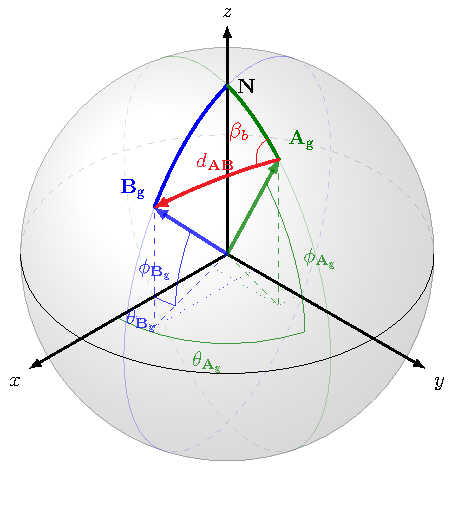
\includegraphics{../pictures/globo.pdf}
    \caption*{Fonte: Autor.}
    \label{fig:globo}
\end{figure}

Calculam-se $\Delta_\phi$ e $\Delta_\theta$.

    \begin{equation}
        \Delta_\phi = \textcolor{Blue}{\phi_B} - \textcolor{Green}{\phi_A}
    \end{equation}
    \begin{equation}
        \Delta_\theta = \textcolor{Blue}{\theta_B} - \textcolor{Green}{\theta_A}
    \end{equation}

Através da lei dos haversines é possível obter a distância mínima $d$ entre as coordenadas, sobre a superfície, e também o ângulo de \textit{Bearing} \textcolor{Red}{$\beta$} formado no vértice \textcolor{Green}{$\mathbf{A}$} do triângulo esférico $\mathbf{N}$\textcolor{Green}{$\mathbf{A}$}\textcolor{Blue}{$\mathbf{B}$} \cite{chrisveness}.
Para o cálculo de distância, os ângulos devem ser tratados em radianos.

\begin{equation}
    X = \cos\left(\textcolor{Blue}{\theta_B}\right)\cdot \sin\left(\Delta_\phi\right)
\end{equation}
\begin{equation}
    Y = \cos\left(\textcolor{Green}{\theta_A}\right)\cdot\sin\left(\textcolor{Blue}{\theta_B}\right) - \sin\left(\textcolor{Green}{\theta_A}\right) \cdot \cos\left(\textcolor{Green}{\theta_B}\right) \cdot \cos\left(\Delta_\phi\right)
\end{equation}
\begin{equation}
    Z = \sin^2\left(\frac{\Delta_\theta}{2}\right) + \cos\left(\textcolor{Blue}{\theta_B}\right) \cdot \cos\left(\textcolor{Green}{\theta_A}\right) \cdot \sin^2\left(\frac{\Delta_\phi}{2}\right)
\end{equation}
\begin{equation}
    \textcolor{Red}{\beta} = \arctan\left(\frac{X}{Y}\right) - \frac{\pi}{2}
\end{equation}
\begin{equation}
    \textcolor{Red}{d} = R_\text{Terra} \cdot 2 \cdot \arctan\left(\frac{\sqrt{Z}}{\sqrt{1-Z}}\right)
\end{equation}

O ângulo \textcolor{Red}{$\beta$} calculado aqui é referente à direção cardeal Norte, assim, uma equipe de busca equipada com uma bússola simples seria capaz de seguir a direção correta.
A \autoref{fig:bearing} apresenta a aplicação desenvolvida por \citeauthor{chrisveness}, capaz de calcular o ângulo de \textit{Bearing} entre duas coordenadas, note que, neste caso, o ângulo referido é relacionado à direção cardial Leste \cite{chrisveness}.

\begin{figure}[htbp]
    \centering
    \caption{Cálculo do ângulo de \textit{Bearing} \textcolor{Red}{$\beta$} entre as coordenadas dos Campi Santo André e São Bernardo do Campo da UFABC.}
    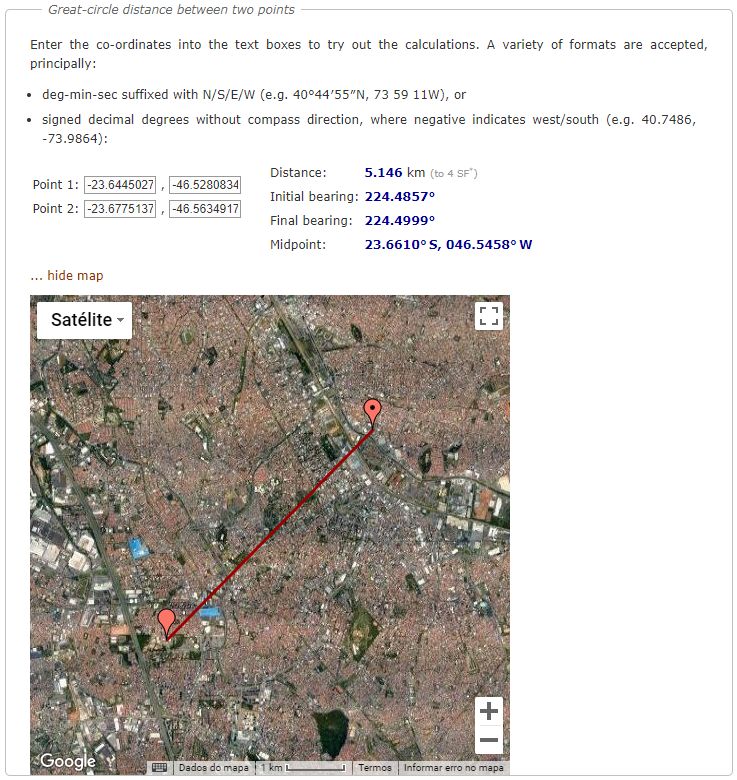
\includegraphics[width=0.7\textwidth]{../pictures/bearing.png}
    \caption*{Fonte: \citeauthor{chrisveness} 2019 \cite{chrisveness}}
    \label{fig:bearing}
\end{figure}

\subsection{Estimar \acs{AoA} utilizando matriz de antenas}

Analisando a defasagem de sinal \ac{RF} em um conjunto de antenas, é possível estimar seu \acf{AoA}, essa técnica pode ser utilizada para determinar a direção do emissor em relação à matriz de antenas utilizada.
Baseando-se em dados como a distância entre as antenas, o comprimento de onda $\lambda$ do sinal e a velocidade da luz no meio, usualmente tomada como $c = \SI{299792458,6 \pm 0,3}{\metre\per\second}$ no ar \cite{jennings1987continuity, bensky2016wireless, horst2021localization}.
A \autoref{eq:wavelength} apresenta a relação do comprimento de onda $\lambda$ com a frequência $f$, com a frequência angular $\omega$ e a velocidade da luz $c$.

\begin{equation}\label{eq:wavelength}
    \lambda = \frac{c}{f} = \frac{2\pi \cdot c}{\omega}
\end{equation}

Se um emissor estiver distante o bastante, é possível considerar que sua frente de onda tem um comportamento planar, essa característica simplifica as operações envolvidas.
A distância de Fraunhofer ($d_F$) é a mínima para essa condição, que define o início da região de \textit{far-field}, conforme apresentado na \autoref{eq:fraunhofer}, onde $D$ é a maior dimensão da antena \cite{balanis2016antenna}.
Tomando $D = 2  \lambda$, para uma antena de dipolo, obtém-se $d_F = 8 \lambda$.
A \autoref{fig:plana_0} ilustra o comportamento planar de uma frente de onda além de $d_F$.

\begin{equation}\label{eq:fraunhofer}
    d_F = \frac{2 \cdot D^2}{\lambda} \quad \Rightarrow \quad d_F = \frac{2 \cdot \left(2 \cdot \lambda \right)^2}{\lambda} = 8 \lambda
\end{equation}

\begin{figure}[htpb]
    \centering
    \caption{Característica de frente de onda a cada $\lambda$ a partir da antena.}
    %     % \resizebox{\textwidth}{!}{%
    \begin{circuitikz}[american, voltage shift=0.5, line width=0.5]

        \def\wavelength{0.5}
        \def\d{0.5*\wavelength}

        \def\closeRange{1}
        \def\farRange{\closeRange+30}

        \coordinate (O) at (0,0);
        \coordinate (antenna) at (-\closeRange,0);
        % \draw [help lines, dashed] (-5,-3) grid (5,3); % desenha grid
        % \draw [red] (O) node[draw,cross out] {}; % marca pont(0,0)

        \draw[thick]
            (antenna) node[dinantenna, scale=0.75]{}
        ;

        % \draw (\closeRange-0.5,-4) rectangle (\farRange+0.1,4);
        \clip (-0.75,-1.5) rectangle (12.1,1.5);
        \foreach \x [evaluate={\z=int((\x+\closeRange));}] in {0,...,30} {
            \draw [gray, thin, opacity=0.5] (antenna) circle (\z*\wavelength);
            \draw [black]
            (antenna) ++ (\z*\wavelength,0)
            node[anchor=south, font = {\footnotesize\bfseries}, rotate=-90,scale=0.75]{$\z\lambda$}
            ++(0, -4)
            -- ++(0,8);
        }

        \draw [Red, thick] (antenna) ++ (8*\wavelength,-4) -- ++(0,8);

        % \foreach \x in {0,60,...,300} {
        %     \draw[thick] (\x:1 cm) -- (\x + 60:1 cm);

        %     \draw (\x + 30:1.732 cm) node[Gray, circ]{};
        %     \draw[Gray, dashed] (\x:1 cm) -- ++(\x: 0.9cm);
        %     \draw[Gray, dotted]
        %     %     % (\x:1 cm) arc (\x+240:\x+180:1cm)
        %         (\x:1 cm) arc [start angle=\x+120, delta angle=110, radius=1cm]
        %         (\x:1 cm) arc [start angle=\x+120, delta angle=-50, radius=1cm]
        %     ;
        % }

        % \draw (0,0) node [circ] {} node [below left,font={\scriptsize\bfseries}] {BS};
        % \draw[thick, densely dotted] (0,0) circle (1cm);

        % \draw[-latex] (0,0) -- (0:1cm) node[midway, below] {$R_c$};
        % \draw[-latex] (0,0) -- (90:0.866cm) node[midway, left] {$R$};

    \end{circuitikz}
  % }

    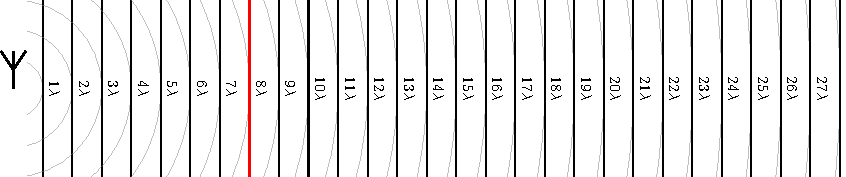
\includegraphics{../pictures/plana_0.pdf}
    \caption*{Fonte: Autor.}
    \label{fig:plana_0}
\end{figure}

Tomando agora um par de antenas separadas por uma distância fixa $d$, torna-se viável fazer a análise trigonométrica entre as antenas e a frente de onda que chega, onde essa distância $d$ será a hipotenusa do triângulo.
A \autoref{fig:AoA} apresenta a disposição das antenas em dois casos de chegada de sinal \ac{RF}.
Para realizar a análise, é necessário conhecer uma segunda dimensão do triângulo retângulo envolvido, esta é obtida analisando a defasagem entre o sinal das antenas, conforme apresentado na \autoref{eq:defasagem}.

\begin{equation}\label{eq:defasagem}
    d \cdot \sin\left(\beta\right) = \lambda \cdot \frac{\Delta\Phi}{2 \pi} \quad \Rightarrow \quad \beta = \arcsin \left(\frac{\lambda}{d} \cdot \frac{\Delta\Phi}{2 \pi}\right)
\end{equation}

É importante ressaltar que um sistemas com um único par de antenas não é capaz de determinar completamente o \ac{AoA}, já que o valor calculado de $\beta$ é igual para casos simétricos, a relação é apresentada nas Figuras \ref{fig:AoA:1} e \ref{fig:AoA:2}.
Existem ainda dois casos notáveis, onde o sinal chega alinhado com a linha das com as antenas ou perpendicular a ela, apresentados respectivamente nas Figuras \ref{fig:AoA:3} e \ref{fig:AoA:4}.

\begin{figure}
    \caption{\ac{AoA} com par de antenas em diversas direções equivalentes.}
    \label{fig:AoA}

    \hfill
    \begin{subfigure}[b]{0.45\textwidth}
        \centering
        \caption{$\beta=\SI{60}{\degree}$}
        % % \resizebox{!}{0.7\textheight}{%
\begin{circuitikz}[american, voltage shift=0.5, line width=0.5, every node/.style={font = {\footnotesize\bfseries}}]

    \def\wavelength{3.5}
    \pgfmathsetmacro\d{0.5*\wavelength}

    \def\antennaAngle{20}
    \pgfmathsetmacro\signalAngle{\antennaAngle+40}

    \def\closeRange{9}
    \def\farRange{\closeRange+13}

	\def\NAntennas{3}
	\pgfmathsetmacro\AngleAntennas{360/\NAntennas}
	\def\ShiftAngleAntennas{-90}

	\pgfmathsetmacro\RhoAntennas{\d/(2*sin(180/\NAntennas))}

    \def\centerarc(#1)(#2:#3:#4)% Syntax: [draw options] (center) (initial angle:final angle:radius)
    { ($(#1)+({#4*cos(#2)},{#4*sin(#2)})$) arc (#2:#3:#4) }

    \def\coordref[#1](#2){%

        \coordinate(sysref) at (#2);

        \draw[#1, -latex] (sysref) ++(-0.4,-0.3) -- ++(0.9,0) node[midway, below]{$x$};
        \draw[#1, -latex] (sysref) ++(-0.3,-0.4) -- ++(0,0.9) node[midway, left]{$y$};
        \draw[#1, -latex] \centerarc(sysref)(-90:180:0.25);
        \draw[#1] (sysref) node{$+$}
    }

    \coordinate (bottomleft) at (-3.5,-1);
    \coordinate (topright) at (3.5,5);


    % \draw[Red,dashed] (bottomleft) rectangle (topright);
    \clip (bottomleft) rectangle (topright);

    \coordinate (O) at (0,0);
    \coordinate (sourceAntenna) at (\signalAngle:\closeRange*\wavelength);
    % \draw [help lines, dashed] (bottomleft) grid (topright); % desenha grid
    % \draw [red] (O) node[draw,cross out] {}; % marca pont(0,0)

    % Circulo de antenas
	% \draw[densely dotted, opacity=0.25] (O) ++(90:\RhoAntennas) circle (\RhoAntennas);

    % Linhas do sinal de fundo
    \foreach \x [evaluate={\y=int((\x+\closeRange));\z=int((\x+\closeRange));}] in {-3,...,3} {
        \draw [black!75, very thin]
        (sourceAntenna) ++ (\signalAngle:-\z*\wavelength)
            % node[anchor=west, font = {\footnotesize\bfseries}]{$\y\lambda$}
        ($(sourceAntenna) + (\signalAngle:-\z*\wavelength) + ({10*cos(\signalAngle+90)},{10*sin(\signalAngle+90)})$)
            --
        ($(sourceAntenna) + (\signalAngle:-\z*\wavelength) - ({10*cos(\signalAngle+90)},{10*sin(\signalAngle+90)})$)
        % \draw [gray, thin] (sourceAntenna) circle (\z)
        ;
    }

    % Antenas
    \draw[thick, cmyk_R] (O) node[dinantenna] (A00) {} ;
    % \draw[thick, cmyk_G, opacity=0.75] (O) ++(60:\d) node[dinantenna] (A0d) {} node [below] {$A_{k+2}$};
    \draw[thick, cmyk_B] (O) ++(\antennaAngle:\d) node[dinantenna] (Ad0) {} ;

    \draw[very thin, Black!50, -latex] % Desenha eixo X
        (-3,0) -- (3,0) node[below left] {$x$}
    ;

    % Ângulo alpha entre antenas
    \draw[thin, cmyk_M]
        \centerarc(O)(0:\antennaAngle:0.3)
        node [above, inner sep=3pt] {$\alpha$}
    ;


    % Desenha senoide de fundo
    \draw[Goldenrod, domain=-8:8, samples=100]
        (A00) ++(\signalAngle+90:0.5*\wavelength) coordinate(signalAux)
        plot[shift={(signalAux)}, rotate=\signalAngle]({\x},{cos(\x * pi * 2 / \wavelength r)})
    ;

    % Direção do sinal
    \draw[very thick, dashed, -latex, Goldenrod]
        % (A00) ++(1.5*\d,0) ++ (\signalAngle:-0.5*\d) -- coordinate(angleArrow) ++(\signalAngle:\d)
        (A00) ++(-2,0) ++ (\signalAngle:-0.25*\d) -- coordinate(angleArrow) ++ (\signalAngle:0.5*\d) --++(\signalAngle:0.25*\d)
    ;
    % Angulo Theta do sinal
    \draw[thin]
        (angleArrow) ++ (0.4, 0) node [below,inner sep=2pt] {$\theta_\text{\ac{AoA}}$}
        \centerarc(angleArrow)(0:\signalAngle:0.4)
    ;

    % Triangulo retângulo + quadradinho
    \draw[Black]

        (A00) --++($({\signalAngle-90}:{\d*sin(\signalAngle-\antennaAngle)})$) coordinate (pontoTriangulo) -- (Ad0) -- (A00)

        (pontoTriangulo)
          ++(\signalAngle:0.125)
        --++(\signalAngle+90:0.125)
        --++(\signalAngle+180:0.125)
    ;

    % Arco do angulo beta
    \draw[thin, Purple]
        (Ad0) ++ (180+\antennaAngle:0.4) node[above, inner sep=3pt] {$\beta$}
        \centerarc(Ad0)(180+\antennaAngle:180+\signalAngle:0.4)
    ;

    % Distânci d entre antenas
    \draw[latex-latex]
        ($(A00)+(0,1)$) -- ($(Ad0)+(0,1)$) node [midway, fill=white, circle, inner sep=1pt] {$d$}
    ;

    \newcommand\CircleRadius{3cm}
    %   \draw (0,0) circle (\CircleRadius);
    % special method of noting the position of a point
    \coordinate (P) at (50:\CircleRadius);

\end{circuitikz}
% }


        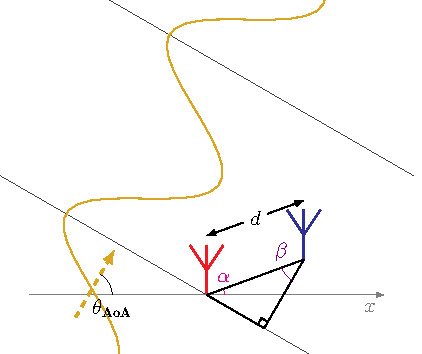
\includegraphics{../pictures/AoA_1.pdf}
        \label{fig:AoA:1}
    \end{subfigure}
    \hfill
    \begin{subfigure}[b]{0.45\textwidth}
        \centering
        \caption{$\beta=\SI{60}{\degree}$}
        %     % \resizebox{!}{0.7\textheight}{%
    \begin{circuitikz}[american, voltage shift=0.5, line width=0.5,every node/.style={font = {\footnotesize\bfseries}}]

        \def\wavelength{3.5}
        \def\d{0.5*\wavelength}

        \def\antennaAngle{210}

        \def\closeRange{9}
        \def\farRange{\closeRange+13}

        \def\centerarc[#1](#2)(#3:#4:#5)% Syntax: [draw options] (center) (initial angle:final angle:radius)
        { \draw[#1] ($(#2)+({#5*cos(#3)},{#5*sin(#3)})$) arc (#3:#4:#5) node[midway,anchor=west] {$\beta$}; }


        \coordinate (O) at (0,0);
        \coordinate (antenna) at (\antennaAngle:\closeRange*\wavelength);
        % \draw [help lines, dashed] (-5,-3) grid (5,3); % desenha grid
        % \draw [red] (O) node[draw,cross out] {}; % marca pont(0,0) 
        
        % \draw (-6.8,-4) rectangle (6.8,4);
        \clip (-3.5,-3.5) rectangle (3.5,3.5);

        % \draw[thick]
        %     (antenna) node[dinantenna]{}
        % ;
        
        \foreach \x [evaluate={\y=int((\x+\closeRange));\z=int((\x+\closeRange));}] in {-3,...,3} {
            \draw [black, thin] 
            (antenna) ++ (\antennaAngle:-\z*\wavelength)
                % node[anchor=west, font = {\footnotesize\bfseries}]{$\y\lambda$}
            ($(antenna) + (\antennaAngle:-\z*\wavelength) + ({10*cos(\antennaAngle+90)},{10*sin(\antennaAngle+90)})$)
                -- 
            ($(antenna) + (\antennaAngle:-\z*\wavelength) - ({10*cos(\antennaAngle+90)},{10*sin(\antennaAngle+90)})$);
            % \draw [gray, thin] (antenna) circle (\z);
        }
        
        \draw[thick]
            (0,0)  node[Green, dinantenna] (A00) {}
            % (0,\d) node[Blue,  dinantenna] (A0d) {}
            (\d,0) node[Red,   dinantenna] (Ad0) {}
        ;

        \draw[very thick, dashed, -latex]
            (A00) ++(-\d,0) coordinate(aux) ++(\antennaAngle:0.5*\d) -- ++(\antennaAngle:-\d)
        ;

        
        \draw[Goldenrod, domain=-8:8, samples=100] plot[shift={(aux)}, rotate=\antennaAngle]({\x},{sin(\x * pi * 2 / \wavelength r)});
        
        \draw[thin, opacity=0.5]
            (A00) ++ ($({\antennaAngle-90}:{\d*sin(\antennaAngle)})$) -- (Ad0) -- (A00)

            ($({\antennaAngle-90}:{\d*sin(\antennaAngle)})$) 
              ++(\antennaAngle+180:0.125)
            --++(\antennaAngle-90:0.125)
            --++(\antennaAngle:0.125)

            
        ;

        \centerarc[thin, opacity=0.5](A00)(\antennaAngle+90:360:0.4)

        \draw[latex-latex]
            ($(A00)+(0,1)$) -- ($(Ad0)+(0,1)$) node [midway, fill=white] {$d$}
        ;
        


        % \foreach \x in {0,60,...,300} {
        %     \draw[thick] (\x:1 cm) -- (\x + 60:1 cm);
            
        %     \draw (\x + 30:1.732 cm) node[Gray, circ]{};
        %     \draw[Gray, dashed] (\x:1 cm) -- ++(\x: 0.9cm);
        %     \draw[Gray, dotted]
        %     %     % (\x:1 cm) arc (\x+240:\x+180:1cm)
        %         (\x:1 cm) arc [start angle=\x+120, delta angle=110, radius=1cm]
        %         (\x:1 cm) arc [start angle=\x+120, delta angle=-50, radius=1cm]
        %     ;
        % }
    
        % \draw (0,0) node [circ] {} node [below left,font={\scriptsize\bfseries}] {BS};
        % \draw[thick, densely dotted] (0,0) circle (1cm);
        
        % \draw[-latex] (0,0) -- (0:1cm) node[midway, below] {$R_c$};
        % \draw[-latex] (0,0) -- (90:0.866cm) node[midway, left] {$R$};
            
    \end{circuitikz}
  % }


        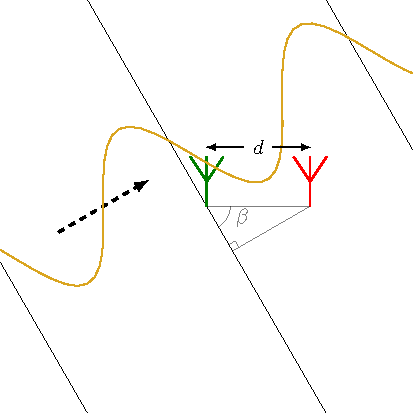
\includegraphics{../pictures/AoA_2.pdf}
        \label{fig:AoA:2}
    \end{subfigure}
    \hfill

    \hfill
    \begin{subfigure}[b]{0.45\textwidth}
        \centering
        \caption{$\beta=\SI{90}{\degree}$}
        %     % \resizebox{!}{0.7\textheight}{%
    \begin{circuitikz}[american, voltage shift=0.5, line width=0.5,every node/.style={font = {\footnotesize\bfseries}}]

        \def\wavelength{3.5}
        \def\d{0.5*\wavelength}


        \def\antennaAngle{180}
        \def\closeRange{9}
        \def\farRange{\closeRange+13}

        \def\centerarc[#1](#2)(#3:#4:#5)% Syntax: [draw options] (center) (initial angle:final angle:radius)
        { \draw[#1] ($(#2)+({#5*cos(#3)},{#5*sin(#3)})$) arc (#3:#4:#5) node[midway,anchor=west] {$\beta$}; }


        \coordinate (O) at (0,0);
        \coordinate (antenna) at (\antennaAngle:\closeRange*\wavelength);
        % \draw [help lines, dashed] (-5,-3) grid (5,3); % desenha grid
        % \draw [red] (O) node[draw,cross out] {}; % marca pont(0,0) 
        
        % \draw (-6.8,-4) rectangle (6.8,4);
        \clip (-3.5,-3.5) rectangle (3.5,3.5);

        % \draw[thick]
        %     (antenna) node[dinantenna]{}
        % ;
        
        \foreach \x [evaluate={\y=int((\x+\closeRange));\z=int((\x+\closeRange));}] in {-3,...,3} {
            \draw [black, thin] 
            (antenna) ++ (\antennaAngle:-\z*\wavelength)
                % node[anchor=west, font = {\footnotesize\bfseries}]{$\y\lambda$}
            ($(antenna) + (\antennaAngle:-\z*\wavelength) + ({10*cos(\antennaAngle+90)},{10*sin(\antennaAngle+90)})$)
                -- 
            ($(antenna) + (\antennaAngle:-\z*\wavelength) - ({10*cos(\antennaAngle+90)},{10*sin(\antennaAngle+90)})$);
            % \draw [gray, thin] (antenna) circle (\z);
        }
        
        \draw[thick]
            (0,0)  node[Green, dinantenna] (A00) {}
            % (0,\d) node[Blue,  dinantenna] (A0d) {}
            (\d,0) node[Red,   dinantenna] (Ad0) {}
        ;

        \draw[very thick, dashed, -latex]
            (A00) ++(-\d,0) coordinate(aux) ++(\antennaAngle:0.5*\d) -- ++(\antennaAngle:-\d)
        ;

        
        \draw[Goldenrod, domain=-8:8, samples=100] plot[shift={(aux)}, rotate=\antennaAngle]({\x},{cos(\x * pi * 2 / \wavelength r)});
        % \draw[thin, densely dotted]
        %     (A00) ++ ($({\antennaAngle-90}:{\d*sin(\antennaAngle)})$) -- (Ad0) -- (A00)

        %     ($({\antennaAngle-90}:{\d*sin(\antennaAngle)})$) 
        %       ++(\antennaAngle+180:0.25)
        %     --++(\antennaAngle-90:0.25)
        %     --++(\antennaAngle:0.25)

            
        % ;

        % \centerarc[thin, densely dotted](A00)(\antennaAngle+90:360:0.4)

        \draw[latex-latex]
            ($(A00)+(0,1)$) -- ($(Ad0)+(0,1)$) node [midway, fill=white] {$d$}
        ;

        % \draw[color=Blue, samples=100, domain=-4:4, smooth]
        %     (A00)++(-\d,0)
        %     % plot[rotate=\antennaAngle] ({\x},{sin((\x r)*0.31830)})
        % ;


        % \foreach \x in {0,60,...,300} {
        %     \draw[thick] (\x:1 cm) -- (\x + 60:1 cm);
            
        %     \draw (\x + 30:1.732 cm) node[Gray, circ]{};
        %     \draw[Gray, dashed] (\x:1 cm) -- ++(\x: 0.9cm);
        %     \draw[Gray, dotted]
        %     %     % (\x:1 cm) arc (\x+240:\x+180:1cm)
        %         (\x:1 cm) arc [start angle=\x+120, delta angle=110, radius=1cm]
        %         (\x:1 cm) arc [start angle=\x+120, delta angle=-50, radius=1cm]
        %     ;
        % }
    
        % \draw (0,0) node [circ] {} node [below left,font={\scriptsize\bfseries}] {BS};
        % \draw[thick, densely dotted] (0,0) circle (1cm);
        
        % \draw[-latex] (0,0) -- (0:1cm) node[midway, below] {$R_c$};
        % \draw[-latex] (0,0) -- (90:0.866cm) node[midway, left] {$R$};
            
    \end{circuitikz}
  % }


        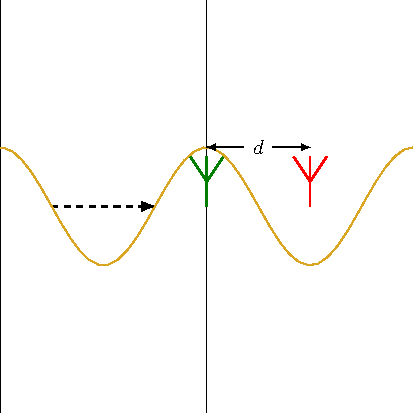
\includegraphics{../pictures/AoA_3.pdf}
        \label{fig:AoA:3}
    \end{subfigure}
    \hfill
    \begin{subfigure}[b]{0.45\textwidth}
        \centering
        \caption{$\beta=\SI{0}{\degree}$}
        % % \resizebox{!}{0.7\textheight}{%
\begin{circuitikz}[american, voltage shift=0.5, line width=0.5, every node/.style={font = {\footnotesize\bfseries}}]

    \def\wavelength{3.5}
    \pgfmathsetmacro\d{0.5*\wavelength}

    \def\antennaAngle{20}
    \def\signalAngle{\antennaAngle}

    \def\closeRange{9}
    \def\farRange{\closeRange+13}

	\def\NAntennas{3}
	\pgfmathsetmacro\AngleAntennas{360/\NAntennas}
	\def\ShiftAngleAntennas{-90}

	\pgfmathsetmacro\RhoAntennas{\d/(2*sin(180/\NAntennas))}

    \def\centerarc(#1)(#2:#3:#4)% Syntax: [draw options] (center) (initial angle:final angle:radius)
    { ($(#1)+({#4*cos(#2)},{#4*sin(#2)})$) arc (#2:#3:#4) }

    \def\coordref[#1](#2){%

        \coordinate(sysref) at (#2);

        \draw[#1, -latex] (sysref) ++(-0.4,-0.3) -- ++(0.9,0) node[midway, below]{$x$};
        \draw[#1, -latex] (sysref) ++(-0.3,-0.4) -- ++(0,0.9) node[midway, left]{$y$};
        \draw[#1, -latex] \centerarc(sysref)(-90:180:0.25);
        \draw[#1] (sysref) node{$+$}
    }

    \coordinate (bottomleft) at (-3.5,-1);
    \coordinate (topright) at (3.5,5);


    % \draw[Red,dashed] (bottomleft) rectangle (topright);
    \clip (bottomleft) rectangle (topright);

    \coordinate (O) at (0,0);
    \coordinate (sourceAntenna) at (\signalAngle:\closeRange*\wavelength);
    % \draw [help lines, dashed] (bottomleft) grid (topright); % desenha grid
    % \draw [red] (O) node[draw,cross out] {}; % marca pont(0,0)

    % Circulo de antenas
	% \draw[densely dotted, opacity=0.25] (O) ++(90:\RhoAntennas) circle (\RhoAntennas);

    % Linhas do sinal de fundo
    \foreach \x [evaluate={\y=int((\x+\closeRange));\z=int((\x+\closeRange));}] in {-3,...,3} {
        \draw [black!75, very thin]
        (sourceAntenna) ++ (\signalAngle:-\z*\wavelength)
            % node[anchor=west, font = {\footnotesize\bfseries}]{$\y\lambda$}
        ($(sourceAntenna) + (\signalAngle:-\z*\wavelength) + ({10*cos(\signalAngle+90)},{10*sin(\signalAngle+90)})$)
            --
        ($(sourceAntenna) + (\signalAngle:-\z*\wavelength) - ({10*cos(\signalAngle+90)},{10*sin(\signalAngle+90)})$)
        % \draw [gray, thin] (sourceAntenna) circle (\z)
        ;
    }

    % Antenas
    \draw[thick, cmyk_R] (O) node[dinantenna] (A00) {} ;
    % \draw[thick, cmyk_G, opacity=0.75] (O) ++(60:\d) node[dinantenna] (A0d) {} node [below] {$A_{k+2}$};
    \draw[thick, cmyk_B] (O) ++(\antennaAngle:\d) node[dinantenna] (Ad0) {} ;

    \draw[very thin, Black!50, -latex] % Desenha eixo X
        (-3,0) -- (3,0) node[below left] {$x$}
    ;

    % Ângulo alpha entre antenas
    \draw[thin, cmyk_M]
		(0.3,0) node [below, inner sep=3pt] {$\alpha$}
		\centerarc(O)(0:\antennaAngle:0.3)
    ;


    % Desenha senoide de fundo
    \draw[Goldenrod, domain=-8:8, samples=100]
        (A00) ++(\signalAngle+90:0.75*\wavelength) coordinate(signalAux)
        plot[shift={(signalAux)}, rotate=\signalAngle]({\x},{cos(\x * pi * 2 / \wavelength r)})
    ;

    % Direção do sinal
    \draw[very thick, dashed, -latex, Goldenrod]
        % (A00) ++(1.5*\d,0) ++ (\signalAngle:-0.25*\d) -- coordinate(angleArrow) ++(\signalAngle:0.85*\d)
        (A00) ++(-2,0) ++ (\signalAngle:-0.25*\d) -- coordinate(angleArrow) ++ (\signalAngle:0.5*\d) --++(\signalAngle:0.25*\d)
    ;
    % Angulo Theta do sinal
    \draw[thin]
        (angleArrow) ++ (0.4, 0) node [below,inner sep=2pt] {$\theta_\text{\ac{AoA}}$}
        \centerarc(angleArrow)(0:\signalAngle:0.4)
    ;

    % Triangulo retângulo + quadradinho
    \draw[Black]

    %     % (A00) --++($({\signalAngle-90}:{\d*sin(\signalAngle-\antennaAngle)})$) coordinate (pontoTriangulo) --
		(Ad0) -- (A00)

    %     % (pontoTriangulo)
    %     %   ++(\signalAngle:0.125)
    %     % --++(\signalAngle+90:0.125)
    %     % --++(\signalAngle+180:0.125)
    ;

    % % Arco do angulo beta
    % \draw[thin]
    %     \centerarc(Ad0)(180+\antennaAngle:180+\signalAngle:0.4) node[below, inner sep=3pt] {$\beta$}
    % ;

    % Distânci d entre antenas
    \draw[latex-latex]
        ($(A00)+(0,1)$) -- ($(Ad0)+(0,1)$) node [midway, fill=white, circle, inner sep=1pt] {$d$}
    ;

    \newcommand\CircleRadius{3cm}
    %   \draw (0,0) circle (\CircleRadius);
    % special method of noting the position of a point
    \coordinate (P) at (50:\CircleRadius);

\end{circuitikz}
% }


        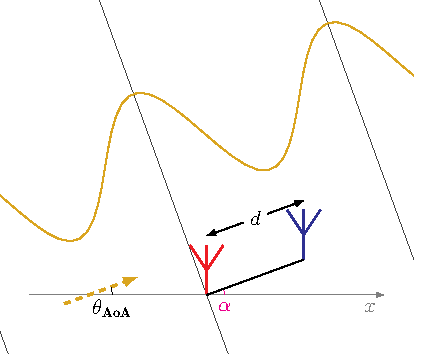
\includegraphics{../pictures/AoA_4.pdf}
        \label{fig:AoA:4}
    \end{subfigure}
    \hfill

    \caption*{Fonte: Autor.}
\end{figure}

A escolha da distância $d$ entre as antenas deve ser feita de forma a otimizar a otimizar a resolução da medida de defasagem, com a maior distância possível, porém é necessário evitar ambiguidades na análise, como o sinal é periódico, o valor se repetirá a cada $\lambda$, e terá valores simétricos quando $d > \sfrac{\lambda}{2}$, ilustrado na \autoref{fig:AoA_d:fail}.
Adota-se então $d=\sfrac{\lambda}{2}$, conforme apresentado na \autoref{fig:AoA_d:ok} \cite{bensky2016wireless, horst2021localization}.

\begin{figure}
    \caption{Diferentes valores para $d$.}
    \label{fig:AoA_d}

    \hfill
    \begin{subfigure}[b]{0.45\textwidth}
        \centering
        \caption{$d > \sfrac{\lambda}{2}$}
        %     % \resizebox{!}{0.7\textheight}{%
    \begin{circuitikz}[american, voltage shift=0.5, line width=0.5,every node/.style={font = {\footnotesize\bfseries}}]

        \def\wavelength{4}
        \def\d{0.5*\wavelength}


        \def\antennaAngle{120}
        \def\closeRange{9}
        \def\farRange{\closeRange+13}

        \def\centerarc[#1](#2)(#3:#4:#5)% Syntax: [draw options] (center) (initial angle:final angle:radius)
        { \draw[#1] ($(#2)+({#5*cos(#3)},{#5*sin(#3)})$) arc (#3:#4:#5) node[midway,anchor=west] {$\beta$}; }


        \coordinate (O) at (0,0);
        \coordinate (antenna) at (\antennaAngle:\closeRange*\wavelength);
        % \draw [help lines, dashed] (-3,-3) grid (3,3); % desenha grid
        % \draw [red] (O) node[draw,cross out] {}; % marca pont(0,0)

        % \draw (-6.8,-4) rectangle (6.8,4);
        \clip (-1,-1.1) rectangle (5,1.1);


        \draw[thick]
            (0,0)  node[cmyk_B, dinantenna] (A00) {}
            % (0,\d) node[Blue,  dinantenna] (A0d) {}
            (1.2*\d,0) node[cmyk_R,   dinantenna] (Ad0) {}
            (0.8*\d,0) node[cmyk_R,   dinantenna, opacity=0.2] (Ad0_phantom) {}
        ;

        % \draw[Goldenrod, domain=-3:3, samples=100] plot[shift={(-1,-1)}, rotate=30]({\x},{sin(\x * pi * 2 / \wavelength r)});
        \draw[Goldenrod, domain=-3:6, samples=50]
            plot ({\x},{cos(\x * pi * 2 / \wavelength r)})
        ;

        \draw[Black, dashed, domain=-3:6, samples=2]
            plot[Black, thin, dashed, samples=2] (\x,0)
        ;

        \draw [densely dotted, cmyk_R]
            (Ad0_phantom) --
            ++(0,{cos(1.2*\d * pi * 2 / \wavelength r)}) --
            ++({0.4*\d},0) --
            (Ad0)
        ;

    \end{circuitikz}
  % }
        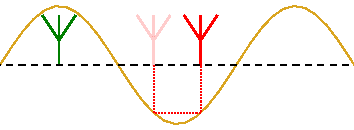
\includegraphics{../pictures/AoA_0_fail.pdf}
        \label{fig:AoA_d:fail}
    \end{subfigure}
    \hfill
    \begin{subfigure}[b]{0.45\textwidth}
        \centering
        \caption{$d = \sfrac{\lambda}{2}$}
        %     % \resizebox{!}{0.7\textheight}{%
    \begin{circuitikz}[american, voltage shift=0.5, line width=0.5,every node/.style={font = {\footnotesize\bfseries}}]

        \def\wavelength{4}
        \def\d{0.5*\wavelength}


        \def\antennaAngle{120}
        \def\closeRange{9}
        \def\farRange{\closeRange+13}

        \def\centerarc[#1](#2)(#3:#4:#5)% Syntax: [draw options] (center) (initial angle:final angle:radius)
        { \draw[#1] ($(#2)+({#5*cos(#3)},{#5*sin(#3)})$) arc (#3:#4:#5) node[midway,anchor=west] {$\beta$}; }


        \coordinate (O) at (0,0);
        \coordinate (antenna) at (\antennaAngle:\closeRange*\wavelength);
        % \draw [help lines, dashed] (-3,-3) grid (3,3); % desenha grid
        % \draw [red] (O) node[draw,cross out] {}; % marca pont(0,0) 
        
        % \draw (5,1.25) rectangle (-1,-1.1);
        \clip (5,1.25) rectangle (-1,-1.1);

        
        % \draw[Goldenrod, domain=-3:3, samples=100] plot[shift={(-1,-1)}, rotate=30]({\x},{sin(\x * pi * 2 / \wavelength r)});
        \draw[Goldenrod, domain=-3:6, samples=50] 
            plot ({\x},{cos(\x * pi * 2 / \wavelength r)})
        ;
        
        \draw[Black, dashed, domain=-3:6, samples=2] 
            plot[Black, thin, dashed, samples=2] (\x,0)
        ;
        
        
        % \pause
        \draw[thick]
            (0,0)  node[Green, dinantenna] (A00) {}
            % (0,\d) node[Blue,  dinantenna] (A0d) {}
            % (\d,0) node[Red,   dinantenna] (Ad0) {}
        ;
        
        % \pause
        \draw[thick]
            % (0,0)  node[Green, dinantenna] (A00) {}
            % (0,\d) node[Blue,  dinantenna] (A0d) {}
            (\d,0) node[Red,   dinantenna] (Ad0) {}
        ;

        \draw[latex-latex]
            ($(A00)+(0,1.1)$) -- ++(\wavelength,0) node [midway, fill=white] {$\lambda$}
        ;
    % \visible<7->{
        \draw[latex-latex]
            ($(A00)+(0,-0.1)$) -- ++(0.5*\wavelength,0) node [midway, fill=white, fill opacity=0.75, anchor=north] {$d = \sfrac{\lambda}{2}$}
        ;
    % }
            
    \end{circuitikz}
  % }
        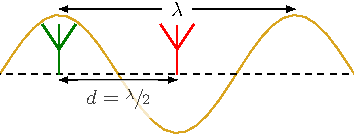
\includegraphics{../pictures/AoA_0.pdf}
        \label{fig:AoA_d:ok}
    \end{subfigure}
    \hfill

    \caption*{Fonte: Autor.}
\end{figure}

Para contornar a ambiguidade gerada pela simetria no sistema, é possível adicionar uma terceira antena, de forma que não esteja alinhada com as duas primeiras.
Um exemplo é apresentado na \autoref{fig:AoA_5}.

\begin{figure}[htbp]
    \centering
    \caption{Possível disposição de matriz de antenas.}
    %     % \resizebox{!}{0.7\textheight}{%
    \begin{circuitikz}[american, voltage shift=0.5, line width=0.5,every node/.style={font = {\footnotesize\bfseries}}]

        \def\wavelength{4}
        \def\d{0.5*\wavelength}


        \def\antennaAngle{240}
        \def\closeRange{9}
        \def\farRange{\closeRange+13}

        \def\centerarc[#1](#2)(#3:#4:#5)(#6)(#7)% Syntax: [draw options] (center) (initial angle:final angle:radius)
        { \draw[#1] ($(#2)+({#5*cos(#3)},{#5*sin(#3)})$) arc (#3:#4:#5) node[midway,anchor=#7] {#6}; }


        \coordinate (O) at (0,0);
        \coordinate (antenna) at (\antennaAngle:\closeRange*\wavelength);
        % \draw [help lines, dashed] (-5,-3) grid (5,3); % desenha grid
        % \draw [red] (O) node[draw,cross out] {}; % marca pont(0,0)

        % \draw (-6.8,-4) rectangle (6.8,4);
        \clip (-6.8,-4) rectangle (6.8,4);

        % \draw[thick]
        %     (antenna) node[dinantenna]{}
        % ;

        \foreach \x [evaluate={\y=int((\x+\closeRange));\z=int((\x+\closeRange)*\wavelength);}] in {-3,...,3} {
            \draw [black, thin]
            (antenna) ++ (\antennaAngle:-\z)
                % node[anchor=west, font = {\footnotesize\bfseries}]{$\y\lambda$}
            ($(antenna) + (\antennaAngle:-\z) + ({10*cos(\antennaAngle+90)},{10*sin(\antennaAngle+90)})$)
                --
            ($(antenna) + (\antennaAngle:-\z) - ({10*cos(\antennaAngle+90)},{10*sin(\antennaAngle+90)})$);
            % \draw [gray, thin] (antenna) circle (\z);
        }

        \draw[thick]
            (0,0)  node[Green, dinantenna] (A00) {}
            (0,\d) node[Blue,  dinantenna] (A0d) {}
            (\d,0) node[Red,   dinantenna] (Ad0) {}
        ;

        \draw[very thick, dashed, -latex]
            (A00) ++(-\d,0) coordinate(aux) ++(\antennaAngle:0.5*\d) -- ++(\antennaAngle:-\d)
        ;


        % \draw[antena_5_5, domain=-8:8, samples=100] plot[shift={(aux)}, rotate=\antennaAngle]({\x},{sin(\x * pi * 2 / \wavelength r)});

        \draw[thin, Red, opacity=0.5]
            (A00) ++ ($({\antennaAngle-90}:{\d*sin(\antennaAngle)})$) -- (Ad0) -- (A00)

            ($({\antennaAngle-90}:{\d*sin(\antennaAngle)})$)
              ++(\antennaAngle+180:0.25)
            --++(\antennaAngle-90:0.25)
            --++(\antennaAngle:0.25)
        ;


        \centerarc[thin, Red, opacity=0.5](A00)(\antennaAngle+90:360:0.4)($\beta_{0d}$)(north)


        \draw[thin, Blue, opacity=0.5]
            (A00) ++ ($({\antennaAngle+90}:{\d*cos(\antennaAngle)})$) -- (A0d) -- (A00)

            ($({\antennaAngle+90}:{\d*cos(\antennaAngle)})$)
              ++(\antennaAngle+180:0.25)
            --++(\antennaAngle+90:0.25)
            --++(\antennaAngle:0.25)
        ;

        \centerarc[thin, Blue, opacity=0.5](A00)(\antennaAngle-90:90:0.4)($\beta_{d0}$)(north east)

        \draw[latex-latex]
            ($(A00)+(0,1)$) -- ($(Ad0)+(0,1)$) node [midway, fill=white] {$d$}
        ;



        % \foreach \x in {0,60,...,300} {
        %     \draw[thick] (\x:1 cm) -- (\x + 60:1 cm);

        %     \draw (\x + 30:1.732 cm) node[Gray, circ]{};
        %     \draw[Gray, dashed] (\x:1 cm) -- ++(\x: 0.9cm);
        %     \draw[Gray, dotted]
        %     %     % (\x:1 cm) arc (\x+240:\x+180:1cm)
        %         (\x:1 cm) arc [start angle=\x+120, delta angle=110, radius=1cm]
        %         (\x:1 cm) arc [start angle=\x+120, delta angle=-50, radius=1cm]
        %     ;
        % }

        % \draw (0,0) node [circ] {} node [below left,font={\scriptsize\bfseries}] {BS};
        % \draw[thick, densely dotted] (0,0) circle (1cm);

        % \draw[-latex] (0,0) -- (0:1cm) node[midway, below] {$R_c$};
        % \draw[-latex] (0,0) -- (90:0.866cm) node[midway, left] {$R$};

    \end{circuitikz}
  % }


    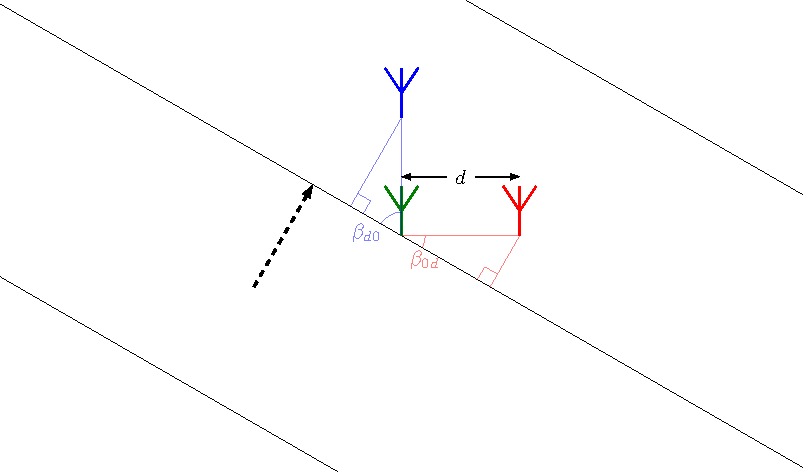
\includegraphics{../pictures/AoA_5.pdf}
    \caption*{Fonte: Autor.}
    \label{fig:AoA_5}
\end{figure}

Para obter o valor de defasagem entre antenas, é interessante representar o sinal recebido como um valor complexo.
Uma forma de obter o valor complexo é realizando a integração de período completo no produto do sinal recebido na antena por uma senoide ou cossenoide de mesma frequência.
Nas Equações \ref{eq:S} e \ref{eq:C}, $S$ e $C$ são respectivamente proporcionais às componentes em fase e em quadratura do sinal $w$ recebido na antena, $k$ é uma função auxiliar que garante frequência correta em todos os operandos.
É válido notar que $w$ e $k$ são funções de várias variáveis.

\begin{equation}\label{eq:S}
    S = \int_0^T w(t) \cdot \sin(k(t)) \partial t
\end{equation}

\begin{equation}\label{eq:C}
    C = \int_0^T w(t) \cdot \cos(k(t)) \partial t
\end{equation}

Finalmente, na \autoref{eq:Z}, $Z$ é o valor complexo associada ao sinal recebido em na antena.

\begin{equation}\label{eq:Z}
    Z_{x,y} = 2\cdot(S + \imath C)
\end{equation}

A defasagem entre um par de antenas é dado pelo ângulo do valor resultante da multiplicação do valor complexo da primeira antena pelo complexo conjugado da segunda antena, conforme apresentado na \autoref{eq:phase}.

\begin{equation}\label{eq:phase}
    \Delta\Phi_{x,y} = \arg(Z_{0,0}\cdot Z^*_{x,y})
\end{equation}

Com este valor é possível estimar valor de $\beta$ no intervalo $\SI{0}{\degree} \leq \beta \leq \SI{180}{\degree}$.

Utilizando a terceira antena perpendicular ao primeiro par e alinhada com uma das antenas iniciais, conforme \autoref{fig:AoA_5}, é possível estimar o valor de $\beta$ no intervalo $\SI{0}{\degree} \leq \beta \leq \SI{360}{\degree}$.
Cada par de antena pode indicar o valor da coordenada geométrica associada ao eixo que a caracteriza, conforme indicado na \autoref{eq:componente}.
Essa propriedade somente é válida nessa geometria.

\begin{equation}\label{eq:componente}
    \text{componente}_{x,y} = -\frac{\Delta_{x,y}}{\pi}\cdot\frac{\cancel{\lambda}}{\cancel{d \cdot 2}} = -\frac{\Delta_{x,y}}{\pi}
\end{equation}

\subsection{AoA aux}

\subsection{Estimar \acs{AoA} utilizando malha de antenas}\label{ssec:aoa}

Analisando a defasagem de um sinal de \ac{RF} incidindo em uma malha de antenas, é possível estimar seu \acf{AoA}, ou seja, determinar a direção do emissor do sinal em relação ao sistema.
Este valor é calculado utilizando dados como a distância entre as antenas, o comprimento de onda \ac{lambda} do sinal e a velocidade da luz no meio, usualmente tomada como $\ac{c} = \SI{299792458,6 \pm 0,3}{\metre\per\second}$ no ar \cite{jennings1987continuity, bensky2016wireless, horst2021localization, Schssel2016AngleOA}.
A \autoref{eq:wavelength} apresenta a relação do comprimento de onda \ac{lambda} com a frequência \ac{f}, a frequência angular \ac{omega} e a velocidade da luz \ac{c}.

% Comprimento de onda
\begin{equation} \label{eq:wavelength}
    \ac{lambda} = \frac{\ac{c}}{\ac{f}} = \frac{2\pi \cdot \ac{c}}{\ac{omega}}
\end{equation}

% {Distância mínima}

Se um emissor de sinal estiver suficientemente distante, é possível considerar que a frente de onda tem um comportamento planar, essa característica simplifica as operações envolvidas.
A distância de Fraunhofer (\ac{dFran}) é a mínima para essa condição, ela define o início da região de \textit{far-field}, conforme apresentado na \autoref{eq:fraunhofer}, onde \ac{D} é a maior dimensão da antena emissora \cite{balanis2016antenna}.
Tomando $ \ac{D} = 2 \ac{lambda}$, para uma antena de dipolo, obtém-se $\ac{dFran} = 8 \ac{lambda} $.
A \autoref{fig:plana_0} ilustra o comportamento planar de uma frente de onda, com destaque na distância \ac{dFran}.

\begin{equation} \label{eq:fraunhofer}
    \ac{dFran} = \frac{2 \cdot \ac{D}^2}{\ac{lambda}} \quad \Rightarrow \quad \ac{dFran} = \frac{2 \cdot \left(2 \cdot \ac{lambda} \right)^2}{\ac{lambda}} = 8 \ac{lambda}
\end{equation}

\begin{figure}[htbp]
    \centering
    \caption{Característica de frente de onda a cada \ac{lambda} a partir da antena emissora, destaque para $\ac{dFran} = 8 \ac{lambda}$.}
        % \resizebox{\textwidth}{!}{%
    \begin{circuitikz}[american, voltage shift=0.5, line width=0.5]

        \def\wavelength{0.5}
        \def\d{0.5*\wavelength}

        \def\closeRange{1}
        \def\farRange{\closeRange+30}

        \coordinate (O) at (0,0);
        \coordinate (antenna) at (-\closeRange,0);
        % \draw [help lines, dashed] (-5,-3) grid (5,3); % desenha grid
        % \draw [red] (O) node[draw,cross out] {}; % marca pont(0,0)

        \draw[thick]
            (antenna) node[dinantenna, scale=0.75]{}
        ;

        % \draw (\closeRange-0.5,-4) rectangle (\farRange+0.1,4);
        \clip (-0.75,-1.5) rectangle (12.1,1.5);
        \foreach \x [evaluate={\z=int((\x+\closeRange));}] in {0,...,30} {
            \draw [gray, thin, opacity=0.5] (antenna) circle (\z*\wavelength);
            \draw [black]
            (antenna) ++ (\z*\wavelength,0)
            node[anchor=south, font = {\footnotesize\bfseries}, rotate=-90,scale=0.75]{$\z\lambda$}
            ++(0, -4)
            -- ++(0,8);
        }

        \draw [Red, thick] (antenna) ++ (8*\wavelength,-4) -- ++(0,8);

        % \foreach \x in {0,60,...,300} {
        %     \draw[thick] (\x:1 cm) -- (\x + 60:1 cm);

        %     \draw (\x + 30:1.732 cm) node[Gray, circ]{};
        %     \draw[Gray, dashed] (\x:1 cm) -- ++(\x: 0.9cm);
        %     \draw[Gray, dotted]
        %     %     % (\x:1 cm) arc (\x+240:\x+180:1cm)
        %         (\x:1 cm) arc [start angle=\x+120, delta angle=110, radius=1cm]
        %         (\x:1 cm) arc [start angle=\x+120, delta angle=-50, radius=1cm]
        %     ;
        % }

        % \draw (0,0) node [circ] {} node [below left,font={\scriptsize\bfseries}] {BS};
        % \draw[thick, densely dotted] (0,0) circle (1cm);

        % \draw[-latex] (0,0) -- (0:1cm) node[midway, below] {$R_c$};
        % \draw[-latex] (0,0) -- (90:0.866cm) node[midway, left] {$R$};

    \end{circuitikz}
  % }

    % 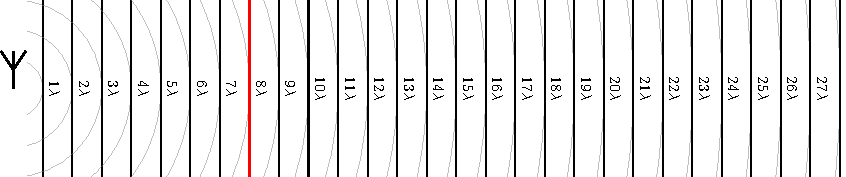
\includegraphics{../pictures/plana_0.pdf}
    \caption*{Fonte: Autor.}
    \label{fig:plana_0}
\end{figure}

% {Trigonometria}

Tomando agora um par de antenas separadas por uma distância fixa \ac{d}, torna-se viável fazer a análise trigonométrica entre as antenas e a frente de onda incidente, onde essa distância \ac{d} será a hipotenusa do triângulo retângulo formado.
Para realizar esta análise, ainda é necessário conhecer uma segunda dimensão do triângulo retângulo envolvido, esta é obtida da defasagem \ac{DeltaPhi} dos sinais incidentes nas antenas, conforme apresentado na \autoref{eq:defasagem}.
A \autoref{fig:AoA} apresenta quatro casos de chegada do sinal de \ac{RF} em um par de antenas.


% Relacao trigonometrica de defasagem e angulo do sinal
\begin{equation} \label{eq:defasagem}
    \ac{d} \cdot
    \cos\left(\textcolor{Purple}{\ac{betak}}\right) =
    \ac{lambda} \cdot
    \frac{\ac{DeltaPhi}}{2 \pi}
\end{equation}


É importante ressaltar que um sistema com um único par de antenas não é suficiente para determinar completamente o \ac{thetaAoA}, já que o valor calculado de \textcolor{Purple}{\ac{betak}} é igual para casos simétricos em relação ao par de antenas, criando um caso de ambiguidade.
As Figuras \ref{fig:AoA:1} e \ref{fig:AoA:2} apresentam exemplos de diferentes valores de \ac{thetaAoA} para o mesmo valor de \textcolor{Purple}{\ac{betak}}.
Existem ainda dois casos notáveis, onde o sinal chega alinhado ao par de antenas ou perpendicular a elas, apresentados respectivamente nas Figuras \ref{fig:AoA:3} e \ref{fig:AoA:4}.

\begin{figure}
    \caption{Diferentes valores de \ac{thetaAoA} para sinal incidente em par de antenas, sistema com ângulo $\textcolor{cmyk_M}{\ac{alphak}}=\SI{20}{\degree}$ em relação à referência.}
    \label{fig:AoA}

    \hfill
    \begin{subfigure}[b]{0.45\textwidth}
        \centering
        \caption{$ \ac{thetaAoA} = \SI{60}{\degree} $, $ \textcolor{Purple}{\ac{betak}} = \SI{40}{\degree} $}
        % \resizebox{!}{0.7\textheight}{%
\begin{circuitikz}[american, voltage shift=0.5, line width=0.5, every node/.style={font = {\footnotesize\bfseries}}]

    \def\wavelength{3.5}
    \pgfmathsetmacro\d{0.5*\wavelength}

    \def\antennaAngle{20}
    \pgfmathsetmacro\signalAngle{\antennaAngle+40}

    \def\closeRange{9}
    \def\farRange{\closeRange+13}

	\def\NAntennas{3}
	\pgfmathsetmacro\AngleAntennas{360/\NAntennas}
	\def\ShiftAngleAntennas{-90}

	\pgfmathsetmacro\RhoAntennas{\d/(2*sin(180/\NAntennas))}

    \def\centerarc(#1)(#2:#3:#4)% Syntax: [draw options] (center) (initial angle:final angle:radius)
    { ($(#1)+({#4*cos(#2)},{#4*sin(#2)})$) arc (#2:#3:#4) }

    \def\coordref[#1](#2){%

        \coordinate(sysref) at (#2);

        \draw[#1, -latex] (sysref) ++(-0.4,-0.3) -- ++(0.9,0) node[midway, below]{$x$};
        \draw[#1, -latex] (sysref) ++(-0.3,-0.4) -- ++(0,0.9) node[midway, left]{$y$};
        \draw[#1, -latex] \centerarc(sysref)(-90:180:0.25);
        \draw[#1] (sysref) node{$+$}
    }

    \coordinate (bottomleft) at (-3.5,-1);
    \coordinate (topright) at (3.5,5);


    % \draw[Red,dashed] (bottomleft) rectangle (topright);
    \clip (bottomleft) rectangle (topright);

    \coordinate (O) at (0,0);
    \coordinate (sourceAntenna) at (\signalAngle:\closeRange*\wavelength);
    % \draw [help lines, dashed] (bottomleft) grid (topright); % desenha grid
    % \draw [red] (O) node[draw,cross out] {}; % marca pont(0,0)

    % Circulo de antenas
	% \draw[densely dotted, opacity=0.25] (O) ++(90:\RhoAntennas) circle (\RhoAntennas);

    % Linhas do sinal de fundo
    \foreach \x [evaluate={\y=int((\x+\closeRange));\z=int((\x+\closeRange));}] in {-3,...,3} {
        \draw [black!75, very thin]
        (sourceAntenna) ++ (\signalAngle:-\z*\wavelength)
            % node[anchor=west, font = {\footnotesize\bfseries}]{$\y\lambda$}
        ($(sourceAntenna) + (\signalAngle:-\z*\wavelength) + ({10*cos(\signalAngle+90)},{10*sin(\signalAngle+90)})$)
            --
        ($(sourceAntenna) + (\signalAngle:-\z*\wavelength) - ({10*cos(\signalAngle+90)},{10*sin(\signalAngle+90)})$)
        % \draw [gray, thin] (sourceAntenna) circle (\z)
        ;
    }

    % Antenas
    \draw[thick, cmyk_R] (O) node[dinantenna] (A00) {} ;
    % \draw[thick, cmyk_G, opacity=0.75] (O) ++(60:\d) node[dinantenna] (A0d) {} node [below] {$A_{k+2}$};
    \draw[thick, cmyk_B] (O) ++(\antennaAngle:\d) node[dinantenna] (Ad0) {} ;

    \draw[very thin, Black!50, -latex] % Desenha eixo X
        (-3,0) -- (3,0) node[below left] {$x$}
    ;

    % Ângulo alpha entre antenas
    \draw[thin, cmyk_M]
        \centerarc(O)(0:\antennaAngle:0.3)
        node [above, inner sep=3pt] {$\alpha$}
    ;


    % Desenha senoide de fundo
    \draw[Goldenrod, domain=-8:8, samples=100]
        (A00) ++(\signalAngle+90:0.5*\wavelength) coordinate(signalAux)
        plot[shift={(signalAux)}, rotate=\signalAngle]({\x},{cos(\x * pi * 2 / \wavelength r)})
    ;

    % Direção do sinal
    \draw[very thick, dashed, -latex, Goldenrod]
        % (A00) ++(1.5*\d,0) ++ (\signalAngle:-0.5*\d) -- coordinate(angleArrow) ++(\signalAngle:\d)
        (A00) ++(-2,0) ++ (\signalAngle:-0.25*\d) -- coordinate(angleArrow) ++ (\signalAngle:0.5*\d) --++(\signalAngle:0.25*\d)
    ;
    % Angulo Theta do sinal
    \draw[thin]
        (angleArrow) ++ (0.4, 0) node [below,inner sep=2pt] {$\theta_\text{\ac{AoA}}$}
        \centerarc(angleArrow)(0:\signalAngle:0.4)
    ;

    % Triangulo retângulo + quadradinho
    \draw[Black]

        (A00) --++($({\signalAngle-90}:{\d*sin(\signalAngle-\antennaAngle)})$) coordinate (pontoTriangulo) -- (Ad0) -- (A00)

        (pontoTriangulo)
          ++(\signalAngle:0.125)
        --++(\signalAngle+90:0.125)
        --++(\signalAngle+180:0.125)
    ;

    % Arco do angulo beta
    \draw[thin, Purple]
        (Ad0) ++ (180+\antennaAngle:0.4) node[above, inner sep=3pt] {$\beta$}
        \centerarc(Ad0)(180+\antennaAngle:180+\signalAngle:0.4)
    ;

    % Distânci d entre antenas
    \draw[latex-latex]
        ($(A00)+(0,1)$) -- ($(Ad0)+(0,1)$) node [midway, fill=white, circle, inner sep=1pt] {$d$}
    ;

    \newcommand\CircleRadius{3cm}
    %   \draw (0,0) circle (\CircleRadius);
    % special method of noting the position of a point
    \coordinate (P) at (50:\CircleRadius);

\end{circuitikz}
% }


        % 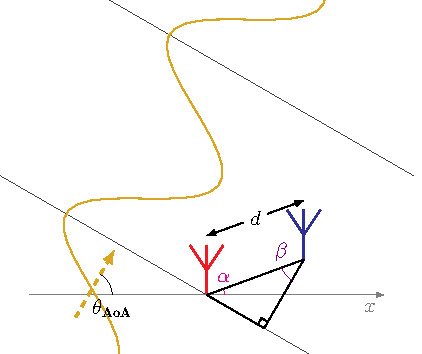
\includegraphics{../pictures/AoA_1.pdf}
        \label{fig:AoA:1}
    \end{subfigure}
    \hfill
    \begin{subfigure}[b]{0.45\textwidth}
        \centering
        \caption{$ \ac{thetaAoA} = \SI{-20}{\degree} $, $ \textcolor{Purple}{\ac{betak}} = \SI{40}{\degree} $}
            % \resizebox{!}{0.7\textheight}{%
    \begin{circuitikz}[american, voltage shift=0.5, line width=0.5,every node/.style={font = {\footnotesize\bfseries}}]

        \def\wavelength{3.5}
        \def\d{0.5*\wavelength}

        \def\antennaAngle{210}

        \def\closeRange{9}
        \def\farRange{\closeRange+13}

        \def\centerarc[#1](#2)(#3:#4:#5)% Syntax: [draw options] (center) (initial angle:final angle:radius)
        { \draw[#1] ($(#2)+({#5*cos(#3)},{#5*sin(#3)})$) arc (#3:#4:#5) node[midway,anchor=west] {$\beta$}; }


        \coordinate (O) at (0,0);
        \coordinate (antenna) at (\antennaAngle:\closeRange*\wavelength);
        % \draw [help lines, dashed] (-5,-3) grid (5,3); % desenha grid
        % \draw [red] (O) node[draw,cross out] {}; % marca pont(0,0) 
        
        % \draw (-6.8,-4) rectangle (6.8,4);
        \clip (-3.5,-3.5) rectangle (3.5,3.5);

        % \draw[thick]
        %     (antenna) node[dinantenna]{}
        % ;
        
        \foreach \x [evaluate={\y=int((\x+\closeRange));\z=int((\x+\closeRange));}] in {-3,...,3} {
            \draw [black, thin] 
            (antenna) ++ (\antennaAngle:-\z*\wavelength)
                % node[anchor=west, font = {\footnotesize\bfseries}]{$\y\lambda$}
            ($(antenna) + (\antennaAngle:-\z*\wavelength) + ({10*cos(\antennaAngle+90)},{10*sin(\antennaAngle+90)})$)
                -- 
            ($(antenna) + (\antennaAngle:-\z*\wavelength) - ({10*cos(\antennaAngle+90)},{10*sin(\antennaAngle+90)})$);
            % \draw [gray, thin] (antenna) circle (\z);
        }
        
        \draw[thick]
            (0,0)  node[Green, dinantenna] (A00) {}
            % (0,\d) node[Blue,  dinantenna] (A0d) {}
            (\d,0) node[Red,   dinantenna] (Ad0) {}
        ;

        \draw[very thick, dashed, -latex]
            (A00) ++(-\d,0) coordinate(aux) ++(\antennaAngle:0.5*\d) -- ++(\antennaAngle:-\d)
        ;

        
        \draw[Goldenrod, domain=-8:8, samples=100] plot[shift={(aux)}, rotate=\antennaAngle]({\x},{sin(\x * pi * 2 / \wavelength r)});
        
        \draw[thin, opacity=0.5]
            (A00) ++ ($({\antennaAngle-90}:{\d*sin(\antennaAngle)})$) -- (Ad0) -- (A00)

            ($({\antennaAngle-90}:{\d*sin(\antennaAngle)})$) 
              ++(\antennaAngle+180:0.125)
            --++(\antennaAngle-90:0.125)
            --++(\antennaAngle:0.125)

            
        ;

        \centerarc[thin, opacity=0.5](A00)(\antennaAngle+90:360:0.4)

        \draw[latex-latex]
            ($(A00)+(0,1)$) -- ($(Ad0)+(0,1)$) node [midway, fill=white] {$d$}
        ;
        


        % \foreach \x in {0,60,...,300} {
        %     \draw[thick] (\x:1 cm) -- (\x + 60:1 cm);
            
        %     \draw (\x + 30:1.732 cm) node[Gray, circ]{};
        %     \draw[Gray, dashed] (\x:1 cm) -- ++(\x: 0.9cm);
        %     \draw[Gray, dotted]
        %     %     % (\x:1 cm) arc (\x+240:\x+180:1cm)
        %         (\x:1 cm) arc [start angle=\x+120, delta angle=110, radius=1cm]
        %         (\x:1 cm) arc [start angle=\x+120, delta angle=-50, radius=1cm]
        %     ;
        % }
    
        % \draw (0,0) node [circ] {} node [below left,font={\scriptsize\bfseries}] {BS};
        % \draw[thick, densely dotted] (0,0) circle (1cm);
        
        % \draw[-latex] (0,0) -- (0:1cm) node[midway, below] {$R_c$};
        % \draw[-latex] (0,0) -- (90:0.866cm) node[midway, left] {$R$};
            
    \end{circuitikz}
  % }


        % 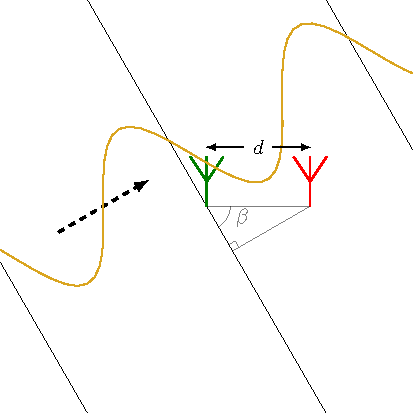
\includegraphics{../pictures/AoA_2.pdf}
        \label{fig:AoA:2}
    \end{subfigure}
    \hfill

    \vspace{\floatsep}

    \hfill
    \begin{subfigure}[b]{0.45\textwidth}
        \centering
        \caption{$ \ac{thetaAoA}=\SI{110}{\degree} $, $ \textcolor{Purple}{\ac{betak}} = \SI{90}{\degree} $}
            % \resizebox{!}{0.7\textheight}{%
    \begin{circuitikz}[american, voltage shift=0.5, line width=0.5,every node/.style={font = {\footnotesize\bfseries}}]

        \def\wavelength{3.5}
        \def\d{0.5*\wavelength}


        \def\antennaAngle{180}
        \def\closeRange{9}
        \def\farRange{\closeRange+13}

        \def\centerarc[#1](#2)(#3:#4:#5)% Syntax: [draw options] (center) (initial angle:final angle:radius)
        { \draw[#1] ($(#2)+({#5*cos(#3)},{#5*sin(#3)})$) arc (#3:#4:#5) node[midway,anchor=west] {$\beta$}; }


        \coordinate (O) at (0,0);
        \coordinate (antenna) at (\antennaAngle:\closeRange*\wavelength);
        % \draw [help lines, dashed] (-5,-3) grid (5,3); % desenha grid
        % \draw [red] (O) node[draw,cross out] {}; % marca pont(0,0) 
        
        % \draw (-6.8,-4) rectangle (6.8,4);
        \clip (-3.5,-3.5) rectangle (3.5,3.5);

        % \draw[thick]
        %     (antenna) node[dinantenna]{}
        % ;
        
        \foreach \x [evaluate={\y=int((\x+\closeRange));\z=int((\x+\closeRange));}] in {-3,...,3} {
            \draw [black, thin] 
            (antenna) ++ (\antennaAngle:-\z*\wavelength)
                % node[anchor=west, font = {\footnotesize\bfseries}]{$\y\lambda$}
            ($(antenna) + (\antennaAngle:-\z*\wavelength) + ({10*cos(\antennaAngle+90)},{10*sin(\antennaAngle+90)})$)
                -- 
            ($(antenna) + (\antennaAngle:-\z*\wavelength) - ({10*cos(\antennaAngle+90)},{10*sin(\antennaAngle+90)})$);
            % \draw [gray, thin] (antenna) circle (\z);
        }
        
        \draw[thick]
            (0,0)  node[Green, dinantenna] (A00) {}
            % (0,\d) node[Blue,  dinantenna] (A0d) {}
            (\d,0) node[Red,   dinantenna] (Ad0) {}
        ;

        \draw[very thick, dashed, -latex]
            (A00) ++(-\d,0) coordinate(aux) ++(\antennaAngle:0.5*\d) -- ++(\antennaAngle:-\d)
        ;

        
        \draw[Goldenrod, domain=-8:8, samples=100] plot[shift={(aux)}, rotate=\antennaAngle]({\x},{cos(\x * pi * 2 / \wavelength r)});
        % \draw[thin, densely dotted]
        %     (A00) ++ ($({\antennaAngle-90}:{\d*sin(\antennaAngle)})$) -- (Ad0) -- (A00)

        %     ($({\antennaAngle-90}:{\d*sin(\antennaAngle)})$) 
        %       ++(\antennaAngle+180:0.25)
        %     --++(\antennaAngle-90:0.25)
        %     --++(\antennaAngle:0.25)

            
        % ;

        % \centerarc[thin, densely dotted](A00)(\antennaAngle+90:360:0.4)

        \draw[latex-latex]
            ($(A00)+(0,1)$) -- ($(Ad0)+(0,1)$) node [midway, fill=white] {$d$}
        ;

        % \draw[color=Blue, samples=100, domain=-4:4, smooth]
        %     (A00)++(-\d,0)
        %     % plot[rotate=\antennaAngle] ({\x},{sin((\x r)*0.31830)})
        % ;


        % \foreach \x in {0,60,...,300} {
        %     \draw[thick] (\x:1 cm) -- (\x + 60:1 cm);
            
        %     \draw (\x + 30:1.732 cm) node[Gray, circ]{};
        %     \draw[Gray, dashed] (\x:1 cm) -- ++(\x: 0.9cm);
        %     \draw[Gray, dotted]
        %     %     % (\x:1 cm) arc (\x+240:\x+180:1cm)
        %         (\x:1 cm) arc [start angle=\x+120, delta angle=110, radius=1cm]
        %         (\x:1 cm) arc [start angle=\x+120, delta angle=-50, radius=1cm]
        %     ;
        % }
    
        % \draw (0,0) node [circ] {} node [below left,font={\scriptsize\bfseries}] {BS};
        % \draw[thick, densely dotted] (0,0) circle (1cm);
        
        % \draw[-latex] (0,0) -- (0:1cm) node[midway, below] {$R_c$};
        % \draw[-latex] (0,0) -- (90:0.866cm) node[midway, left] {$R$};
            
    \end{circuitikz}
  % }


        % 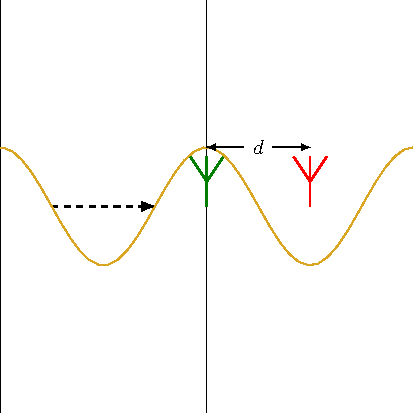
\includegraphics{../pictures/AoA_3.pdf}
        \label{fig:AoA:3}
    \end{subfigure}
    \hfill
    \begin{subfigure}[b]{0.45\textwidth}
        \centering
        \caption{$ \ac{thetaAoA}=\SI{20}{\degree} $, $ \textcolor{Purple}{\ac{betak}} = \SI{0}{\degree} $}
        % \resizebox{!}{0.7\textheight}{%
\begin{circuitikz}[american, voltage shift=0.5, line width=0.5, every node/.style={font = {\footnotesize\bfseries}}]

    \def\wavelength{3.5}
    \pgfmathsetmacro\d{0.5*\wavelength}

    \def\antennaAngle{20}
    \def\signalAngle{\antennaAngle}

    \def\closeRange{9}
    \def\farRange{\closeRange+13}

	\def\NAntennas{3}
	\pgfmathsetmacro\AngleAntennas{360/\NAntennas}
	\def\ShiftAngleAntennas{-90}

	\pgfmathsetmacro\RhoAntennas{\d/(2*sin(180/\NAntennas))}

    \def\centerarc(#1)(#2:#3:#4)% Syntax: [draw options] (center) (initial angle:final angle:radius)
    { ($(#1)+({#4*cos(#2)},{#4*sin(#2)})$) arc (#2:#3:#4) }

    \def\coordref[#1](#2){%

        \coordinate(sysref) at (#2);

        \draw[#1, -latex] (sysref) ++(-0.4,-0.3) -- ++(0.9,0) node[midway, below]{$x$};
        \draw[#1, -latex] (sysref) ++(-0.3,-0.4) -- ++(0,0.9) node[midway, left]{$y$};
        \draw[#1, -latex] \centerarc(sysref)(-90:180:0.25);
        \draw[#1] (sysref) node{$+$}
    }

    \coordinate (bottomleft) at (-3.5,-1);
    \coordinate (topright) at (3.5,5);


    % \draw[Red,dashed] (bottomleft) rectangle (topright);
    \clip (bottomleft) rectangle (topright);

    \coordinate (O) at (0,0);
    \coordinate (sourceAntenna) at (\signalAngle:\closeRange*\wavelength);
    % \draw [help lines, dashed] (bottomleft) grid (topright); % desenha grid
    % \draw [red] (O) node[draw,cross out] {}; % marca pont(0,0)

    % Circulo de antenas
	% \draw[densely dotted, opacity=0.25] (O) ++(90:\RhoAntennas) circle (\RhoAntennas);

    % Linhas do sinal de fundo
    \foreach \x [evaluate={\y=int((\x+\closeRange));\z=int((\x+\closeRange));}] in {-3,...,3} {
        \draw [black!75, very thin]
        (sourceAntenna) ++ (\signalAngle:-\z*\wavelength)
            % node[anchor=west, font = {\footnotesize\bfseries}]{$\y\lambda$}
        ($(sourceAntenna) + (\signalAngle:-\z*\wavelength) + ({10*cos(\signalAngle+90)},{10*sin(\signalAngle+90)})$)
            --
        ($(sourceAntenna) + (\signalAngle:-\z*\wavelength) - ({10*cos(\signalAngle+90)},{10*sin(\signalAngle+90)})$)
        % \draw [gray, thin] (sourceAntenna) circle (\z)
        ;
    }

    % Antenas
    \draw[thick, cmyk_R] (O) node[dinantenna] (A00) {} ;
    % \draw[thick, cmyk_G, opacity=0.75] (O) ++(60:\d) node[dinantenna] (A0d) {} node [below] {$A_{k+2}$};
    \draw[thick, cmyk_B] (O) ++(\antennaAngle:\d) node[dinantenna] (Ad0) {} ;

    \draw[very thin, Black!50, -latex] % Desenha eixo X
        (-3,0) -- (3,0) node[below left] {$x$}
    ;

    % Ângulo alpha entre antenas
    \draw[thin, cmyk_M]
		(0.3,0) node [below, inner sep=3pt] {$\alpha$}
		\centerarc(O)(0:\antennaAngle:0.3)
    ;


    % Desenha senoide de fundo
    \draw[Goldenrod, domain=-8:8, samples=100]
        (A00) ++(\signalAngle+90:0.75*\wavelength) coordinate(signalAux)
        plot[shift={(signalAux)}, rotate=\signalAngle]({\x},{cos(\x * pi * 2 / \wavelength r)})
    ;

    % Direção do sinal
    \draw[very thick, dashed, -latex, Goldenrod]
        % (A00) ++(1.5*\d,0) ++ (\signalAngle:-0.25*\d) -- coordinate(angleArrow) ++(\signalAngle:0.85*\d)
        (A00) ++(-2,0) ++ (\signalAngle:-0.25*\d) -- coordinate(angleArrow) ++ (\signalAngle:0.5*\d) --++(\signalAngle:0.25*\d)
    ;
    % Angulo Theta do sinal
    \draw[thin]
        (angleArrow) ++ (0.4, 0) node [below,inner sep=2pt] {$\theta_\text{\ac{AoA}}$}
        \centerarc(angleArrow)(0:\signalAngle:0.4)
    ;

    % Triangulo retângulo + quadradinho
    \draw[Black]

    %     % (A00) --++($({\signalAngle-90}:{\d*sin(\signalAngle-\antennaAngle)})$) coordinate (pontoTriangulo) --
		(Ad0) -- (A00)

    %     % (pontoTriangulo)
    %     %   ++(\signalAngle:0.125)
    %     % --++(\signalAngle+90:0.125)
    %     % --++(\signalAngle+180:0.125)
    ;

    % % Arco do angulo beta
    % \draw[thin]
    %     \centerarc(Ad0)(180+\antennaAngle:180+\signalAngle:0.4) node[below, inner sep=3pt] {$\beta$}
    % ;

    % Distânci d entre antenas
    \draw[latex-latex]
        ($(A00)+(0,1)$) -- ($(Ad0)+(0,1)$) node [midway, fill=white, circle, inner sep=1pt] {$d$}
    ;

    \newcommand\CircleRadius{3cm}
    %   \draw (0,0) circle (\CircleRadius);
    % special method of noting the position of a point
    \coordinate (P) at (50:\CircleRadius);

\end{circuitikz}
% }


        % 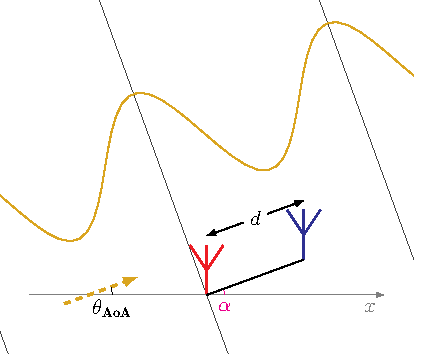
\includegraphics{../pictures/AoA_4.pdf}
        \label{fig:AoA:4}
    \end{subfigure}
    \hfill

    \caption*{Fonte: Autor.}
\end{figure}

% {Distância entre antenas}

A escolha da distância \ac{d} entre as antenas deve ser feita de forma a otimizar a resolução da medida de defasagem, com a maior distância possível. Porém é necessário evitar ambiguidades na análise, por se tratar de um sinal periódico, o valor se repetirá a cada \ac{lambda}, e terá valores simétricos quando $\ac{d} > \sfrac{\ac{lambda}}{2}$, ilustrado na \autoref{fig:AoA_d:fail}.
Adota-se então $\ac{d}=\sfrac{\ac{lambda}}{2}$, conforme apresentado na \autoref{fig:AoA_d:ok} e \autoref{eq:distancia} \cite{bensky2016wireless, horst2021localization, Schssel2016AngleOA}.

\begin{figure}[htbp]
    \caption{Diferentes valores para \ac{d}.}
    \label{fig:AoA_d}

    \hfill
    \begin{subfigure}[b]{0.45\textwidth}
        \centering
        \caption{$\ac{d} > \sfrac{\ac{lambda}}{2}$}
            % \resizebox{!}{0.7\textheight}{%
    \begin{circuitikz}[american, voltage shift=0.5, line width=0.5,every node/.style={font = {\footnotesize\bfseries}}]

        \def\wavelength{4}
        \def\d{0.5*\wavelength}


        \def\antennaAngle{120}
        \def\closeRange{9}
        \def\farRange{\closeRange+13}

        \def\centerarc[#1](#2)(#3:#4:#5)% Syntax: [draw options] (center) (initial angle:final angle:radius)
        { \draw[#1] ($(#2)+({#5*cos(#3)},{#5*sin(#3)})$) arc (#3:#4:#5) node[midway,anchor=west] {$\beta$}; }


        \coordinate (O) at (0,0);
        \coordinate (antenna) at (\antennaAngle:\closeRange*\wavelength);
        % \draw [help lines, dashed] (-3,-3) grid (3,3); % desenha grid
        % \draw [red] (O) node[draw,cross out] {}; % marca pont(0,0)

        % \draw (-6.8,-4) rectangle (6.8,4);
        \clip (-1,-1.1) rectangle (5,1.1);


        \draw[thick]
            (0,0)  node[cmyk_B, dinantenna] (A00) {}
            % (0,\d) node[Blue,  dinantenna] (A0d) {}
            (1.2*\d,0) node[cmyk_R,   dinantenna] (Ad0) {}
            (0.8*\d,0) node[cmyk_R,   dinantenna, opacity=0.2] (Ad0_phantom) {}
        ;

        % \draw[Goldenrod, domain=-3:3, samples=100] plot[shift={(-1,-1)}, rotate=30]({\x},{sin(\x * pi * 2 / \wavelength r)});
        \draw[Goldenrod, domain=-3:6, samples=50]
            plot ({\x},{cos(\x * pi * 2 / \wavelength r)})
        ;

        \draw[Black, dashed, domain=-3:6, samples=2]
            plot[Black, thin, dashed, samples=2] (\x,0)
        ;

        \draw [densely dotted, cmyk_R]
            (Ad0_phantom) --
            ++(0,{cos(1.2*\d * pi * 2 / \wavelength r)}) --
            ++({0.4*\d},0) --
            (Ad0)
        ;

    \end{circuitikz}
  % }
        % 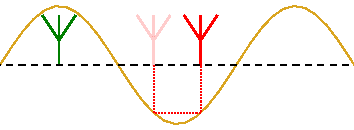
\includegraphics{../pictures/AoA_0_fail.pdf}
        \label{fig:AoA_d:fail}
    \end{subfigure}
    \hfill
    \begin{subfigure}[b]{0.45\textwidth}
        \centering
        \caption{$\ac{d} = \sfrac{\ac{lambda}}{2}$}
            % \resizebox{!}{0.7\textheight}{%
    \begin{circuitikz}[american, voltage shift=0.5, line width=0.5,every node/.style={font = {\footnotesize\bfseries}}]

        \def\wavelength{4}
        \def\d{0.5*\wavelength}


        \def\antennaAngle{120}
        \def\closeRange{9}
        \def\farRange{\closeRange+13}

        \def\centerarc[#1](#2)(#3:#4:#5)% Syntax: [draw options] (center) (initial angle:final angle:radius)
        { \draw[#1] ($(#2)+({#5*cos(#3)},{#5*sin(#3)})$) arc (#3:#4:#5) node[midway,anchor=west] {$\beta$}; }


        \coordinate (O) at (0,0);
        \coordinate (antenna) at (\antennaAngle:\closeRange*\wavelength);
        % \draw [help lines, dashed] (-3,-3) grid (3,3); % desenha grid
        % \draw [red] (O) node[draw,cross out] {}; % marca pont(0,0) 
        
        % \draw (5,1.25) rectangle (-1,-1.1);
        \clip (5,1.25) rectangle (-1,-1.1);

        
        % \draw[Goldenrod, domain=-3:3, samples=100] plot[shift={(-1,-1)}, rotate=30]({\x},{sin(\x * pi * 2 / \wavelength r)});
        \draw[Goldenrod, domain=-3:6, samples=50] 
            plot ({\x},{cos(\x * pi * 2 / \wavelength r)})
        ;
        
        \draw[Black, dashed, domain=-3:6, samples=2] 
            plot[Black, thin, dashed, samples=2] (\x,0)
        ;
        
        
        % \pause
        \draw[thick]
            (0,0)  node[Green, dinantenna] (A00) {}
            % (0,\d) node[Blue,  dinantenna] (A0d) {}
            % (\d,0) node[Red,   dinantenna] (Ad0) {}
        ;
        
        % \pause
        \draw[thick]
            % (0,0)  node[Green, dinantenna] (A00) {}
            % (0,\d) node[Blue,  dinantenna] (A0d) {}
            (\d,0) node[Red,   dinantenna] (Ad0) {}
        ;

        \draw[latex-latex]
            ($(A00)+(0,1.1)$) -- ++(\wavelength,0) node [midway, fill=white] {$\lambda$}
        ;
    % \visible<7->{
        \draw[latex-latex]
            ($(A00)+(0,-0.1)$) -- ++(0.5*\wavelength,0) node [midway, fill=white, fill opacity=0.75, anchor=north] {$d = \sfrac{\lambda}{2}$}
        ;
    % }
            
    \end{circuitikz}
  % }
        % 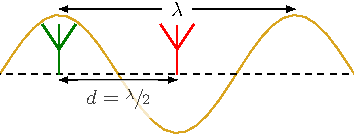
\includegraphics{../pictures/AoA_0.pdf}
        \label{fig:AoA_d:ok}
    \end{subfigure}
    \hfill

    \caption*{Fonte: Autor.}
\end{figure}

\begin{equation} \label{eq:distancia} % Distancia entre par de antenas
    \ac{d} = \frac{\ac{lambda}}{2}
\end{equation}

% % {Ambiguidade simétrica}

Para contornar a ambiguidade de simetria, é possível adicionar mais antenas à malha.
O conjunto de \ac{Nant} antenas deve respeitar a distância \ac{d} entre as antenas de um par, e pode ser disposto como um polígono regular com \ac{Nant} lados de tamanho \ac{d}, onde cada antena está em um vértice.
A \autoref{fig:antennas} apresenta exemplos dessa disposição de antenas, note que valores pares de \ac{Nant} implicam que existirão pares de antenas paralelos, que resultam em leituras redundantes.

\begin{figure}[htbp]
    \centering
    \caption{Diferentes distribuições de antenas.}
    \label{fig:antennas}

    \hfill
    \begin{subfigure}[c]{0.4\textwidth}
        \centering
        \caption{$ \ac{Nant} = 3 $.}
        % % \resizebox{!}{0.7\textheight}{%
\begin{circuitikz}[american, voltage shift=0.5, line width=0.5,every node/.style={font = {\footnotesize\bfseries}}]

    \def\wavelength{8}
    \pgfmathsetmacro\d{0.5*\wavelength}

    \def\signalAngle{75}
    \def\antennaAngle{120}

    \def\closeRange{9}
    \def\farRange{\closeRange+13}

	\def\NAntennas{3}
	\pgfmathsetmacro\AngleAntennas{360/\NAntennas}
	\def\ShiftAngleAntennas{-90}

	\pgfmathsetmacro\RhoAntennas{\d/(2*sin(180/\NAntennas))}

    \def\centerarc(#1)(#2:#3:#4)% Syntax: [draw options] (center) (initial angle:final angle:radius)
    { ($(#1)+({#4*cos(#2)},{#4*sin(#2)})$) arc (#2:#3:#4) }

    \def\coordref[#1](#2){%

        \coordinate(sysref) at (#2);

        \draw[#1, -latex] (sysref) ++(-0.4,-0.3) -- ++(0.9,0) node[midway, below]{$x$};
        \draw[#1, -latex] (sysref) ++(-0.3,-0.4) -- ++(0,0.9) node[midway, left]{$y$};
        \draw[#1, -latex] \centerarc(sysref)(-90:180:0.25);
        \draw[#1] (sysref) node{$+$}
    }

    \coordinate (bottomleft) at (-3,-3);
    \coordinate (topright) at (3,3);


    % \draw[Red,dashed] (bottomleft) rectangle (topright);
    \clip (bottomleft) rectangle (topright);

    \coordinate (O) at (0,0);
    \coordinate (sourceAntenna) at (\signalAngle:\closeRange*\wavelength);
    % \draw [help lines, dashed] (bottomleft) grid (topright); % desenha grid
    % \draw [red] (O) node[draw,cross out] {}; % marca pont(0,0)

	\draw[densely dotted] (O) circle (\RhoAntennas);

    \draw[thick, cmyk_G] (O) ++(1*\AngleAntennas+\ShiftAngleAntennas:\RhoAntennas) node[dinantenna] (A1) {} node [above right] {$A_{1}$};
    \draw[thick, cmyk_B] (O) ++(2*\AngleAntennas+\ShiftAngleAntennas:\RhoAntennas) node[dinantenna] (A2) {} node [above left] {$A_{2}$};
    \draw[thick, cmyk_R] (O) ++(3*\AngleAntennas+\ShiftAngleAntennas:\RhoAntennas) node[dinantenna] (A3) {};

	\coordinate (A1_2) at ($(A1)!0.5!(A2)$);

	\draw[Black!25, dotted]
		(A1) --
		(A3) --
		(A2)
	;

	\draw[Black!50, densely dotted]
		(O) --
		(A2) --
		(A1_2)
	;

	\draw
		(A1) --
		(O) --
		(A1_2) --
		(A1)
	;

	\draw
         (A1_2)
           ++(0:0.125)
         --++(-90:0.125)
         --++(+180:0.125)
	;

	\node at (O) {\tiny\textbullet};

	\draw
		(O) ++(90:0.3) node[left, inner sep=1.5pt] {$\textstyle \frac{\pi}{N_\text{ant}}$}
		\centerarc(O)(1*\AngleAntennas+\ShiftAngleAntennas:90:0.3)
	;


    % Distânci d entre antenas
    \draw[latex-latex]
        ($(A1)+(0,1)$) -- ($(A2)+(0,1)$) node [midway, fill=white, circle, inner sep=1pt] {$d$}
    ;

    \draw[decorate, decoration={brace, amplitude=5pt}, thin]
    ($(A1)+({1*\AngleAntennas+\ShiftAngleAntennas-90}:0.1)$)
    -- coordinate (brace)
    ($(O)+({1*\AngleAntennas+\ShiftAngleAntennas-90}:0.1)$)
    ;

    \draw (brace) ++({1*\AngleAntennas+\ShiftAngleAntennas-90}:5pt)
        node[anchor=north west, circle, fill=white, inner sep=1pt] {$\rho$}
    ;

	\draw[decorate, decoration={brace, amplitude=5pt}, thin]
    ($(A1_2)+({90}:0.1)$)
    -- coordinate (brace)
    ($(A1)+({90}:0.1)$)
    ;

    \draw (brace) ++({90}:5pt)
        node[anchor=south, circle, inner sep=1pt] {$\sfrac{d}{2}$}
    ;

    % \coordref[Black!25](3.5,0);

\end{circuitikz}
% }


        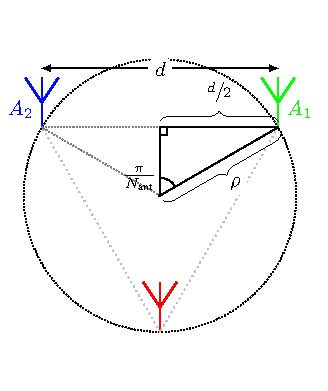
\includegraphics{../pictures/antennas_3.pdf}
        \label{fig:antennas:3}
    \end{subfigure}
    \hfill
    \begin{subfigure}[c]{0.575\textwidth}
        \centering
        \caption{$ \ac{Nant} = 6 $.}
        % % \resizebox{!}{0.7\textheight}{%
\begin{circuitikz}[american, voltage shift=0.5, line width=0.5,every node/.style={font = {\footnotesize\bfseries}}]

    \def\wavelength{8}
    \pgfmathsetmacro\d{0.5*\wavelength}

    \def\signalAngle{75}
    \def\antennaAngle{120}

    \def\closeRange{9}
    \def\farRange{\closeRange+13}

	\def\NAntennas{6}
	\pgfmathsetmacro\AngleAntennas{360/\NAntennas}
	\pgfmathsetmacro\ShiftAngleAntennas{-90+1.5*\AngleAntennas}

	\pgfmathsetmacro\RhoAntennas{\d/(2*sin(180/\NAntennas))}

    \def\centerarc(#1)(#2:#3:#4)% Syntax: [draw options] (center) (initial angle:final angle:radius)
    { ($(#1)+({#4*cos(#2)},{#4*sin(#2)})$) arc (#2:#3:#4) }

    \def\coordref[#1](#2){%

        \coordinate(sysref) at (#2);

        \draw[#1, -latex] (sysref) ++(-0.4,-0.3) -- ++(0.9,0) node[midway, below]{$x$};
        \draw[#1, -latex] (sysref) ++(-0.3,-0.4) -- ++(0,0.9) node[midway, left]{$y$};
        \draw[#1, -latex] \centerarc(sysref)(-90:180:0.25);
        \draw[#1] (sysref) node{$+$}
    }

    \coordinate (bottomleft) at (-4.5,-4.5);
    \coordinate (topright) at (4.5,4.5);


    % \draw[Red,dashed] (bottomleft) rectangle (topright);
    \clip (bottomleft) rectangle (topright);

    \coordinate (O) at (0,0);
    \coordinate (sourceAntenna) at (\signalAngle:\closeRange*\wavelength);
    % \draw [help lines, dashed] (bottomleft) grid (topright); % desenha grid
    % \draw [red] (O) node[draw,cross out] {}; % marca pont(0,0)

	\draw[densely dotted] (O) circle (\RhoAntennas);

    \draw[thick, cmyk_G] (O) ++(1*\AngleAntennas+\ShiftAngleAntennas:\RhoAntennas) node[dinantenna] (A1) {} node [above right] {$A_{1}$};
    \draw[thick, cmyk_B] (O) ++(2*\AngleAntennas+\ShiftAngleAntennas:\RhoAntennas) node[dinantenna] (A2) {} node [above left] {$A_{2}$};
    \draw[thick, cmyk_R] (O) ++(3*\AngleAntennas+\ShiftAngleAntennas:\RhoAntennas) node[dinantenna] (A3) {};
    \draw[thick, cmyk_C] (O) ++(4*\AngleAntennas+\ShiftAngleAntennas:\RhoAntennas) node[dinantenna] (A4) {};
    \draw[thick, cmyk_M] (O) ++(5*\AngleAntennas+\ShiftAngleAntennas:\RhoAntennas) node[dinantenna] (A5) {};
    \draw[thick, DarkGoldenrod] (O) ++(6*\AngleAntennas+\ShiftAngleAntennas:\RhoAntennas) node[dinantenna] (A6) {};

	\coordinate (A1_2) at ($(A1)!0.5!(A2)$);

	\draw[Black!25, dotted]
		(A1) --
		(A6) --
		(A5) --
		(A4) --
		(A3) --
		(A2)
	;

	\draw[Black!50, densely dotted]
		(O) --
		(A2) --
		(A1_2)
	;

	\draw
		(A1) --
		(O) --
		(A1_2) --
		(A1)
	;

	\draw
         (A1_2)
           ++(0:0.125)
         --++(-90:0.125)
         --++(+180:0.125)
	;

	\node at (O) {\tiny\textbullet};

	\draw
		(O) ++(90:0.3) node[left, inner sep=1.5pt] {$\textstyle \frac{\pi}{N_\text{ant}}$}
		\centerarc(O)(1*\AngleAntennas+\ShiftAngleAntennas:90:0.3)
	;


    % Distânci d entre antenas
    \draw[latex-latex]
        ($(A1)+(0,1)$) -- ($(A2)+(0,1)$) node [midway, fill=white, circle, inner sep=1pt] {$d$}
    ;

    \draw[decorate, decoration={brace, amplitude=5pt}, thin]
    ($(A1)+({1*\AngleAntennas+\ShiftAngleAntennas-90}:0.1)$)
    -- coordinate (brace)
    ($(O)+({1*\AngleAntennas+\ShiftAngleAntennas-90}:0.1)$)
    ;

    \draw (brace) ++({1*\AngleAntennas+\ShiftAngleAntennas-90}:5pt)
        node[anchor=north west, circle, fill=white, inner sep=1pt] {$\rho$}
    ;

	\draw[decorate, decoration={brace, amplitude=5pt}, thin]
    ($(A1_2)+({90}:0.1)$)
    -- coordinate (brace)
    ($(A1)+({90}:0.1)$)
    ;

    \draw (brace) ++({90}:5pt)
        node[anchor=south, circle, inner sep=1pt] {$\sfrac{d}{2}$}
    ;

    % \coordref[Black!25](3.5,0);

\end{circuitikz}
% }


        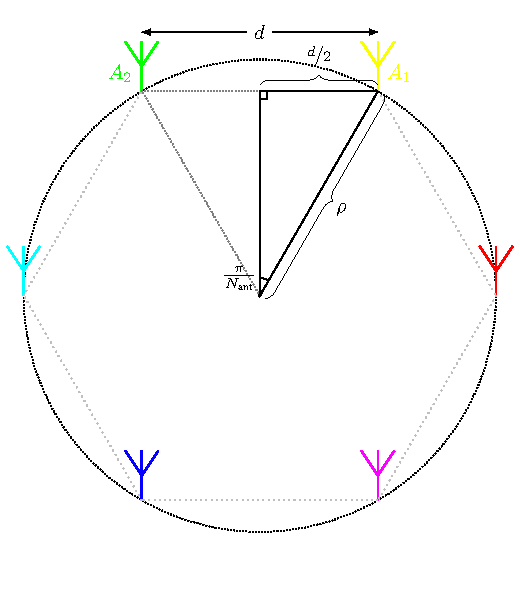
\includegraphics{../pictures/antennas_6.pdf}
        \label{fig:antennas:6}
    \end{subfigure}
    \hfill

    \vspace{\floatsep}

    \hfill
    \begin{subfigure}[c]{0.425\textwidth}
        \centering
        \caption{$ \ac{Nant} = 4 $.}
        % % \resizebox{!}{0.7\textheight}{%
\begin{circuitikz}[american, voltage shift=0.5, line width=0.5,every node/.style={font = {\footnotesize\bfseries}}]

    \def\wavelength{8}
    \pgfmathsetmacro\d{0.5*\wavelength}

    \def\signalAngle{75}
    \def\antennaAngle{120}

    \def\closeRange{9}
    \def\farRange{\closeRange+13}

	\def\NAntennas{4}
	\pgfmathsetmacro\AngleAntennas{360/\NAntennas}
	\pgfmathsetmacro\ShiftAngleAntennas{-90+0.5*\AngleAntennas}

	\pgfmathsetmacro\RhoAntennas{\d/(2*sin(180/\NAntennas))}

    \def\centerarc(#1)(#2:#3:#4)% Syntax: [draw options] (center) (initial angle:final angle:radius)
    { ($(#1)+({#4*cos(#2)},{#4*sin(#2)})$) arc (#2:#3:#4) }

    \def\coordref[#1](#2){%

        \coordinate(sysref) at (#2);

        \draw[#1, -latex] (sysref) ++(-0.4,-0.3) -- ++(0.9,0) node[midway, below]{$x$};
        \draw[#1, -latex] (sysref) ++(-0.3,-0.4) -- ++(0,0.9) node[midway, left]{$y$};
        \draw[#1, -latex] \centerarc(sysref)(-90:180:0.25);
        \draw[#1] (sysref) node{$+$}
    }

    \pgfmathsetmacro\vSize{\RhoAntennas + 1}
    \pgfmathsetmacro\hSize{\RhoAntennas + 0.4}

    \coordinate (bottomleft) at (-\hSize,-\vSize);
    \coordinate (topright) at (\hSize,\vSize);


    % \draw[Red,dashed] (bottomleft) rectangle (topright);
    \clip (bottomleft) rectangle (topright);

    \coordinate (O) at (0,0);
    \coordinate (sourceAntenna) at (\signalAngle:\closeRange*\wavelength);
    % \draw [help lines, dashed] (bottomleft) grid (topright); % desenha grid
    % \draw [red] (O) node[draw,cross out] {}; % marca pont(0,0)

	\draw[densely dotted] (O) circle (\RhoAntennas);

    \draw[thick, antena_4_1] (O) ++(1*\AngleAntennas+\ShiftAngleAntennas:\RhoAntennas) node[dinantenna] (A1) {} node [above right] {$A_{1}$};
    \draw[thick, antena_4_2] (O) ++(2*\AngleAntennas+\ShiftAngleAntennas:\RhoAntennas) node[dinantenna] (A2) {} node [above left] {$A_{2}$};
    \draw[thick, antena_4_3] (O) ++(3*\AngleAntennas+\ShiftAngleAntennas:\RhoAntennas) node[dinantenna] (A3) {};
    \draw[thick, antena_4_4] (O) ++(4*\AngleAntennas+\ShiftAngleAntennas:\RhoAntennas) node[dinantenna] (A4) {};
    % \draw[thick, cmyk_M] (O) ++(5*\AngleAntennas+\ShiftAngleAntennas:\RhoAntennas) node[dinantenna] (A5) {};

	\coordinate (A1_2) at ($(A1)!0.5!(A2)$);

	\draw[Black!25, dotted]
		(A1) --
		(A4) --
		(A3) --
		(A2)
	;

	\draw[Black!50, densely dotted]
		(O) --
		(A2) --
		(A1_2)
	;

	\draw
		(A1) --
		(O) --
		(A1_2) --
		(A1)
	;

	\draw
         (A1_2)
           ++(0:0.125)
         --++(-90:0.125)
         --++(+180:0.125)
	;

	\node at (O) {\tiny\textbullet};

	\draw
		(O) ++(90:0.3) node[left, inner sep=1.5pt] {$\textstyle \frac{\pi}{N_\text{ant}}$}
		\centerarc(O)(1*\AngleAntennas+\ShiftAngleAntennas:90:0.3)
	;


    % Distânci d entre antenas
    \draw[latex-latex]
        ($(A1)+(0,1)$) -- ($(A2)+(0,1)$) node [midway, fill=white, circle, inner sep=1pt] {$d$}
    ;

    \draw[decorate, decoration={brace, amplitude=5pt}, thin]
    ($(A1)+({1*\AngleAntennas+\ShiftAngleAntennas-90}:0.1)$)
    -- coordinate (brace)
    ($(O)+({1*\AngleAntennas+\ShiftAngleAntennas-90}:0.1)$)
    ;

    \draw (brace) ++({1*\AngleAntennas+\ShiftAngleAntennas-90}:5pt)
        node[anchor=north west, circle, fill=white, inner sep=1pt] {$\rho$}
    ;

	\draw[decorate, decoration={brace, amplitude=5pt}, thin]
    ($(A1_2)+({90}:0.1)$)
    -- coordinate (brace)
    ($(A1)+({90}:0.1)$)
    ;

    \draw (brace) ++({90}:5pt)
        node[anchor=south, circle, inner sep=1pt] {$\sfrac{d}{2}$}
    ;

    % \coordref[Black!25](3.5,0);

\end{circuitikz}
% }


        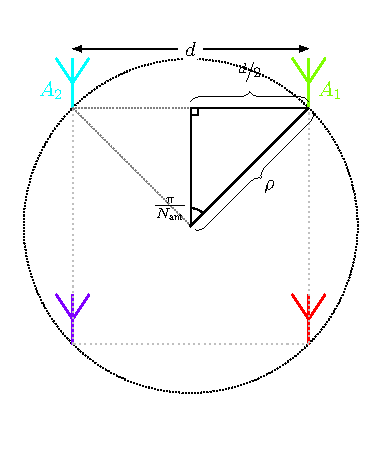
\includegraphics{../pictures/antennas_4.pdf}
        \label{fig:antennas:4}
    \end{subfigure}
    \hfill
    \begin{subfigure}[c]{0.525\textwidth}
        \centering
        \caption{$ \ac{Nant} = 5 $.}
        % % \resizebox{!}{0.7\textheight}{%
\begin{circuitikz}[american, voltage shift=0.5, line width=0.5,every node/.style={font = {\footnotesize\bfseries}}]

    \def\wavelength{8}
    \pgfmathsetmacro\d{0.5*\wavelength}

    \def\signalAngle{75}
    \def\antennaAngle{120}

    \def\closeRange{9}
    \def\farRange{\closeRange+13}

	\def\NAntennas{5}
	\pgfmathsetmacro\AngleAntennas{360/\NAntennas}
	\pgfmathsetmacro\ShiftAngleAntennas{-90+\AngleAntennas}

	\pgfmathsetmacro\RhoAntennas{\d/(2*sin(180/\NAntennas))}

    \def\centerarc(#1)(#2:#3:#4)% Syntax: [draw options] (center) (initial angle:final angle:radius)
    { ($(#1)+({#4*cos(#2)},{#4*sin(#2)})$) arc (#2:#3:#4) }

    \def\coordref[#1](#2){%

        \coordinate(sysref) at (#2);

        \draw[#1, -latex] (sysref) ++(-0.4,-0.3) -- ++(0.9,0) node[midway, below]{$x$};
        \draw[#1, -latex] (sysref) ++(-0.3,-0.4) -- ++(0,0.9) node[midway, left]{$y$};
        \draw[#1, -latex] \centerarc(sysref)(-90:180:0.25);
        \draw[#1] (sysref) node{$+$}
    }

    \coordinate (bottomleft) at (-4,-4);
    \coordinate (topright) at (4,4);


    % \draw[Red,dashed] (bottomleft) rectangle (topright);
    \clip (bottomleft) rectangle (topright);

    \coordinate (O) at (0,0);
    \coordinate (sourceAntenna) at (\signalAngle:\closeRange*\wavelength);
    % \draw [help lines, dashed] (bottomleft) grid (topright); % desenha grid
    % \draw [red] (O) node[draw,cross out] {}; % marca pont(0,0)

	\draw[densely dotted] (O) circle (\RhoAntennas);

    \draw[thick, cmyk_G] (O) ++(1*\AngleAntennas+\ShiftAngleAntennas:\RhoAntennas) node[dinantenna] (A1) {} node [above right] {$A_{1}$};
    \draw[thick, cmyk_B] (O) ++(2*\AngleAntennas+\ShiftAngleAntennas:\RhoAntennas) node[dinantenna] (A2) {} node [above left] {$A_{2}$};
    \draw[thick, cmyk_R] (O) ++(3*\AngleAntennas+\ShiftAngleAntennas:\RhoAntennas) node[dinantenna] (A3) {};
    \draw[thick, cmyk_C] (O) ++(4*\AngleAntennas+\ShiftAngleAntennas:\RhoAntennas) node[dinantenna] (A4) {};
    \draw[thick, cmyk_M] (O) ++(5*\AngleAntennas+\ShiftAngleAntennas:\RhoAntennas) node[dinantenna] (A5) {};

	\coordinate (A1_2) at ($(A1)!0.5!(A2)$);

	\draw[Black!25, dotted]
		(A1) --
		(A5) --
		(A4) --
		(A3) --
		(A2)
	;

	\draw[Black!50, densely dotted]
		(O) --
		(A2) --
		(A1_2)
	;

	\draw
		(A1) --
		(O) --
		(A1_2) --
		(A1)
	;

	\draw
         (A1_2)
           ++(0:0.125)
         --++(-90:0.125)
         --++(+180:0.125)
	;

	\node at (O) {\tiny\textbullet};

	\draw
		(O) ++(90:0.3) node[left, inner sep=1.5pt] {$\textstyle \frac{\pi}{N_\text{ant}}$}
		\centerarc(O)(1*\AngleAntennas+\ShiftAngleAntennas:90:0.3)
	;


    % Distânci d entre antenas
    \draw[latex-latex]
        ($(A1)+(0,1)$) -- ($(A2)+(0,1)$) node [midway, fill=white, circle, inner sep=1pt] {$d$}
    ;

    \draw[decorate, decoration={brace, amplitude=5pt}, thin]
    ($(A1)+({1*\AngleAntennas+\ShiftAngleAntennas-90}:0.1)$)
    -- coordinate (brace)
    ($(O)+({1*\AngleAntennas+\ShiftAngleAntennas-90}:0.1)$)
    ;

    \draw (brace) ++({1*\AngleAntennas+\ShiftAngleAntennas-90}:5pt)
        node[anchor=north west, circle, fill=white, inner sep=1pt] {$\rho$}
    ;

	\draw[decorate, decoration={brace, amplitude=5pt}, thin]
    ($(A1_2)+({90}:0.1)$)
    -- coordinate (brace)
    ($(A1)+({90}:0.1)$)
    ;

    \draw (brace) ++({90}:5pt)
        node[anchor=south, circle, inner sep=1pt] {$\sfrac{d}{2}$}
    ;

    % \coordref[Black!25](3.5,0);

\end{circuitikz}
% }


        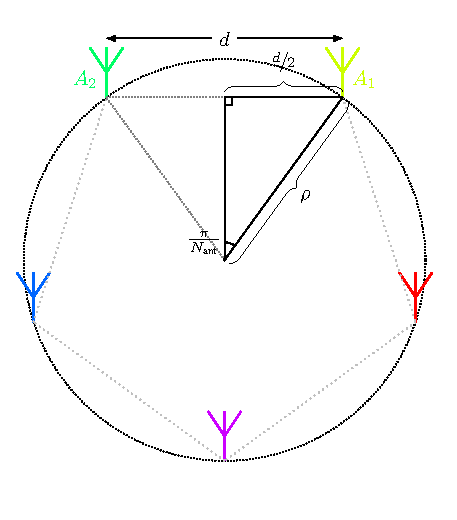
\includegraphics{../pictures/antennas_5.pdf}
        \label{fig:antennas:5}
    \end{subfigure}
    \hfill

    \caption*{Fonte: Autor.}
\end{figure}

A \autoref{eq:raio:poligono} descreve o raio \ac{rho} do círculo que circunscreve o polígono regular de \ac{Nant} antenas.
Este raio equivale à distância das antenas em relação ao ponto central do polígono.

\begin{equation} \label{eq:raio:poligono} % Diametro do circulo que circunscreve poligono de antenas
	\ac{rho} = \frac{\ac{d}}{2\cdot \sin\left(\displaystyle\frac{\pi}{\ac{Nant}}\right)}
\end{equation}

Cada antena é identificada por um índice \ac{k}, conforme a \autoref{eq:ant:idx}, e tem sua coordenada espacial definida como um valor complexo descrito na \autoref{eq:ant:coord}.
Essas coordenadas são definidas como números complexos para simplificar a análise do ângulo \textcolor{cmyk_M}{\ac{alphak}} em que um par de antenas \textcolor{cmyk_B}{\ac{Ak}} e $\textcolor{cmyk_R}{A_{k+1}}$ se dispõe em relação à geometria do sistema, conforme \autoref{eq:ant:angle}.

\begin{equation} \label{eq:ant:idx} % Indices das antenas
	\ac{k} = \left\{1, 2, \dotsc, \ac{Nant}\right\}
\end{equation}

% Coordenada da antena
\begin{equation} \label{eq:ant:coord}
	\textcolor{cmyk_B}{\ac{Ak}} =
    \ac{rho}
    \cdot \exp\left(\ac{imath}\cdot \ac{k} \cdot \frac{2\pi}{\ac{Nant}}\right) =
    \left( \operatorname{\mathcal{Re}}\left( \textcolor{cmyk_B}{\ac{Ak}} \right), ~\operatorname{\mathcal{Im}}\left( \textcolor{cmyk_B}{\ac{Ak}} \right) \right) =
    \left( \ac{xk}, ~ \ac{yk} \right)
\end{equation}

% Angulo do par de antenas
\begin{equation} \label{eq:ant:angle}
	\textcolor{cmyk_M}{\ac{alphak}} = \arg\left( \textcolor{cmyk_B}{\ac{Ak}} - \textcolor{cmyk_R}{A_{k+1}} \right)
\end{equation}

% {Calcular fase}

Para calcular a fase em uma antena, é interessante representar o sinal recebido como um valor complexo.
Uma forma de obter o complexo de fase consiste em analisar a correlação do sinal incidente \ac{w} com sinais de referência de mesma frequência que o sinal de interesse, em um período completo, \autoref{eq:periodo}.
Os valors \ac{Ik} (em fase) e \ac{Qk} (em quadratura) são calculados respectivamente pela correlação com um cosseno, conforme \autoref{eq:in_phase}, e com um seno, conforme \autoref{eq:out_of_phase}.
A \autoref{eq:Z} apresenta o valor complexo \textcolor{cmyk_B}{\ac{Zk}} de fase para a antena \textcolor{cmyk_B}{\ac{Ak}}.


% Periodo do sinal
\begin{equation} \label{eq:periodo}
    \ac{T} = \frac{2\pi}{\ac{omega}} = \frac{1}{\ac{f}}
\end{equation}

% In phase
\begin{equation} \label{eq:in_phase}
    \ac{Ik} =
    \int\limits_0^{\ac{T}} \cos\left(\ac{omega} \cdot\tau\right)
    \cdot \ac{w}\left( \ac{xk}, ~\ac{yk}, ~\tau \right) \partial \tau
\end{equation}

% Out of phase
\begin{equation} \label{eq:out_of_phase}
    \ac{Qk} =
    \int\limits_0^{\ac{T}} \sin\left(\ac{omega}\cdot\tau\right)
    \cdot \ac{w}\left( \ac{xk}, ~\ac{yk}, ~\tau \right) \partial \tau
\end{equation}

% Fase na antena
\begin{equation} \label{eq:Z}
    \textcolor{cmyk_B}{\ac{Zk}} =
    \frac{\ac{omega}}{\pi}\cdot\left(\ac{Ik} + \ac{imath} \ac{Qk}\right)
\end{equation}

% {Calcular defasagem entre antenas}

O cálculo de defasagem de sinal em um par de antenas consiste na análise de diferença de fase dos valores \textcolor{cmyk_B}{\ac{Zk}} e $\textcolor{cmyk_R}{Z_{k+1}}$ do par de antenas \textcolor{cmyk_B}{\ac{Ak}} e $\textcolor{cmyk_R}{A_{k+1}}$, conforme apresentado na \autoref{eq:dephase}.
Obtido o valor de defasagem \ac{DeltaPhi} entre o par de antenas, finalmente é possível calcular o ângulo \textcolor{Purple}{\ac{betak}} através da \autoref{eq:beta}, note que a simplificação somente é possível com valor de $\ac{d} = \sfrac{\ac{lambda}}{2}$.
A \autoref{fig:AoA:geometria} apresenta a geometria do sistema destacando os valores de interesse na análise de um dos pares de antenas, tomando $\ac{Nant} = 3$.

% Defasagem entre antenas
\begin{equation} \label{eq:dephase}
    \ac{DeltaPhi} =
    \textcolor{cmyk_B}{\ac{Phik}} - \textcolor{cmyk_R}{\Phi_{k+1}} =
    \arg\left(\textcolor{cmyk_B}{\ac{Zk}}\right) - \arg\left(\textcolor{cmyk_R}{Z_{k+1}}\right) =
    \arg\left(\textcolor{cmyk_B}{\ac{Zk}} \cdot \overline{\textcolor{cmyk_R}{Z_{k+1}}}\right)
\end{equation}

% Angulo do sinal em relação ao par de antenas
\begin{equation} \label{eq:beta}
    \textcolor{Purple}{\ac{betak}} = \arccos\left(\frac{\cancel{\ac{lambda}}}{\cancel{d}}\cdot\frac{\ac{DeltaPhi}}{\cancel{2}\pi}\right)
\end{equation}

\begin{figure}[htbp]
    \centering
    \caption{Geometria geral do sistema com $\ac{Nant} = 3$.}
    % \resizebox{!}{0.7\textheight}{%
\begin{circuitikz}[american, voltage shift=0.5, line width=0.5, every node/.style={font = {\footnotesize\bfseries}}]

    \def\wavelength{5}
    \pgfmathsetmacro\d{0.5*\wavelength}

    \def\signalAngle{75}
    \def\antennaAngle{120}

    \def\closeRange{9}
    \def\farRange{\closeRange+13}

	\def\NAntennas{3}
	\pgfmathsetmacro\AngleAntennas{360/\NAntennas}
	\def\ShiftAngleAntennas{-90}

	\pgfmathsetmacro\RhoAntennas{\d/(2*sin(180/\NAntennas))}

    \def\centerarc(#1)(#2:#3:#4)% Syntax: [draw options] (center) (initial angle:final angle:radius)
    { ($(#1)+({#4*cos(#2)},{#4*sin(#2)})$) arc (#2:#3:#4) }

    \def\coordref[#1](#2){%

        \coordinate(sysref) at (#2);

        \draw[#1, -latex] (sysref) ++(-0.4,-0.3) -- ++(0.9,0) node[midway, below]{$x$};
        \draw[#1, -latex] (sysref) ++(-0.3,-0.4) -- ++(0,0.9) node[midway, left]{$y$};
        \draw[#1, -latex] \centerarc(sysref)(-90:180:0.25);
        \draw[#1] (sysref) node{$+$}
    }

    \coordinate (bottomleft) at (-6,-0.5);
    \coordinate (topright) at (6,6.5);


    % \draw[Red,dashed] (bottomleft) rectangle (topright);
    \clip (bottomleft) rectangle (topright);

    \coordinate (O) at (0,0);
    \coordinate (sourceAntenna) at (\signalAngle:\closeRange*\wavelength);
    % \draw [help lines, dashed] (bottomleft) grid (topright); % desenha grid
    % \draw [red] (O) node[draw,cross out] {}; % marca pont(0,0)

    % Circulo de antenas
	\draw[densely dotted, opacity=0.25] (O) ++(90:\RhoAntennas) circle (\RhoAntennas);

    % Linhas do sinal de fundo
    \foreach \x [evaluate={\y=int((\x+\closeRange));\z=int((\x+\closeRange));}] in {-3,...,3} {
        \draw [black!75, very thin]
        (sourceAntenna) ++ (\signalAngle:-\z*\wavelength)
            % node[anchor=west, font = {\footnotesize\bfseries}]{$\y\lambda$}
        ($(sourceAntenna) + (\signalAngle:-\z*\wavelength) + ({10*cos(\signalAngle+90)},{10*sin(\signalAngle+90)})$)
            --
        ($(sourceAntenna) + (\signalAngle:-\z*\wavelength) - ({10*cos(\signalAngle+90)},{10*sin(\signalAngle+90)})$)
        % \draw [gray, thin] (sourceAntenna) circle (\z)
        ;
    }

    % Antenas
    \draw[thick, cmyk_R] (O) node[dinantenna] (A00) {} node [below] {$A_{k+1}$};
    \draw[thick, cmyk_G, opacity=0.75] (O) ++(60:\d) node[dinantenna] (A0d) {} node [below] {$A_{k+2}$};
    \draw[thick, cmyk_B] (O) ++(\antennaAngle:\d) node[dinantenna] (Ad0) {} node [above left] {$A_{k}$};

    \draw[very thin, Black!50] % Desenha eixo X
        (-0.5*\d,0) -- (2*\d,0) node[right] {$x$}
    ;

    % Ângulo alpha entre antenas
    \draw[thin, cmyk_M]
        (0.3,0) node [above right, inner sep=1pt] {\ac{alphak}}
        \centerarc(O)(0:\antennaAngle:0.3)
    ;

    % Comprimento de onda
    \draw[latex-latex]
        (A00) ++(\signalAngle+90:\wavelength) coordinate(signalAux)
         -- node [midway, fill=white, circle, inner sep=1pt] {$\lambda$} ++(\signalAngle:\wavelength)
    ;

    % Desenha senoide de fundo
    \draw[Goldenrod, domain=-8:8, samples=100] plot[shift={(signalAux)}, rotate=\signalAngle]({\x},{cos(\x * pi * 2 / \wavelength r)});

    % Direção do sinal
    \draw[very thick, dashed, -latex, Goldenrod]
        (A00) ++(1.5*\d,0) ++ (\signalAngle:-0.5*\d) -- coordinate(angleArrow) ++(\signalAngle:\d)
    ;
    % Angulo Theta do sinal
    \draw[thin]
        \centerarc(angleArrow)(0:\signalAngle:0.4) node [midway,above right,inner sep=1pt] {\ac{thetaAoA}}
    ;

    % Triangulo retângulo + quadradinho
    \draw[Black]

        (A00) --++($({\signalAngle-90}:{\d*sin(\signalAngle-\antennaAngle)})$) coordinate (pontoTriangulo) -- (Ad0) -- (A00)

        (pontoTriangulo)
          ++(\signalAngle:0.125)
        --++(\signalAngle-90:0.125)
        --++(\signalAngle+180:0.125)
    ;
    % Arco do angulo beta
    \draw[thin, Purple] \centerarc(Ad0)(180+\antennaAngle:180+\signalAngle:0.4)
        (Ad0) ++ (180+\signalAngle:0.5) node[below right, inner sep=1pt, fill=white, fill opacity=0.75,] {\ac{betak}}
    ;

    % Distânci d entre antenas
    \draw[latex-latex]
        ($(A00)+(0,1)$) -- ($(Ad0)+(0,1)$) node [midway, fill=white, circle, inner sep=1pt] {\ac{d}}
    ;

    \newcommand\CircleRadius{3cm}
    % special method of noting the position of a point
    \coordinate (P) at (50:\CircleRadius);

    \draw[decorate, decoration={brace, amplitude=5pt}, thin]
    ($(pontoTriangulo)+({\signalAngle+90}:0.1)$)
    -- coordinate (brace)
    ($(Ad0)+({\signalAngle+90}:0.1)$)
    ;

    \draw (brace) ++({\signalAngle+90}:5pt)
        node[anchor=east] {$\displaystyle\ac{lambda} \cdot \frac{\ac{DeltaPhi}}{2 \pi}$}
    ;

    \coordref[Black!25](3,3);

    % \foreach \x in {0,60,...,300} {
    %     \draw[thick] (\x:1 cm) -- (\x + 60:1 cm);

    %     \draw (\x + 30:1.732 cm) node[Gray, circ]{};
    %     \draw[Gray, dashed] (\x:1 cm) -- ++(\x: 0.9cm);
    %     \draw[Gray, dotted]
    %     %     % (\x:1 cm) arc (\x+240:\x+180:1cm)
    %         (\x:1 cm) arc [start angle=\x+120, delta angle=110, radius=1cm]
    %         (\x:1 cm) arc [start angle=\x+120, delta angle=-50, radius=1cm]
    %     ;
    % }

    % \draw (0,0) node [circ] {} node [below left,font={\scriptsize\bfseries}] {BS};
    % \draw[thick, densely dotted] (0,0) circle (1cm);

    % \draw[-latex] (0,0) -- (0:1cm) node[midway, below] {$R_c$};
    % \draw[-latex] (0,0) -- (90:0.866cm) node[midway, left] {$R$};

\end{circuitikz}
% }


    \label{fig:AoA:geometria}
    \caption*{Fonte: Autor.}
\end{figure}

Para cada par de antenas, são calculados dois valores \ac{thetak} conforme a \autoref{eq:theta:pmk}, equivalentes a dois valores possíveis para o \ac{thetaAoA}.
A \autoref{eq:theta:conj} define o conjunto \ac{Theta} dos valores aferidos de \ac{thetak} para todos os pares de antenas do sistema, este conjunto sempre terá $2 \cdot \ac{Nant}$ elementos, dos quais, metade estão próximos do real valor de \ac{thetaAoA} e os demais são valores distintos do objetivo e entre si.

% Conjunto de angulos calculados
\begin{equation} \label{eq:theta:pmk}
	\ac{thetak} = \textcolor{cmyk_M}{\ac{alphak}}\pm \textcolor{Purple}{\ac{betak}}
\end{equation}

% Conjunto de angulos calculados
\begin{equation} \label{eq:theta:conj}
	\ac{Theta} = \left\{\ac{thetak} ~\middle\vert~ \forall \ac{k}\right\}
\end{equation}

% {Escolha dos possíveis angulos}

Com os possíveis valores de \ac{thetaAoA} obtidos, é necessário estimar qual o valor correto.
Para isso, é criada uma lista auxiliar \ac{ThetaQuanti}, quantizando os valores de \ac{Theta} em intervalos de tamanho \ac{delta}, descrito na \autoref{eq:delta:range}.
A \autoref{eq:theta:quant} descreve a operação de quantização dos valores de \ac{Theta}, que, por se tratar de um cálculo auxiliar, utiliza-se o arredondamento para o inteiro mais próximo.
A quantização implica que os valores de \ac{Theta} serão agrupados por faixas de largura \ac{delta}.

% range_angle
\begin{equation} \label{eq:delta:range}
    \ac{delta} = \frac{\pi}{2 \cdot \left( 1 + \ac{Nant} \right)}
\end{equation}

% Angulos normalizados
\begin{equation} \label{eq:theta:quant}
    \ac{ThetaQuanti} =
    \left\{\left\lfloor\frac{\theta}{\ac{delta}}\right\rceil\cdot\ac{delta} ~\middle\vert~ \forall \theta \in \ac{Theta}  \right\}
\end{equation}

Salvo casos com muito ruído, espera-se que alguns valores em \ac{ThetaQuanti} se repitam, partindo disso, calcula-se \ac{thetaMo}, a moda estatística destes valores, conforme \autoref{eq:theta:moda}.
Esse valor deverá estar próximo ao \ac{thetaAoA}, e será utilizado na filtragem dos valores aferidos em \ac{Theta}.

% Moda entre angulos normalizados
\begin{equation} \label{eq:theta:moda}
    \ac{thetaMo} = \operatorname{\mathcal{M_o}}\left( \ac{ThetaQuanti}  \right)
\end{equation}

O conjunto \ac{ThetaFiltro} contém itens de \ac{Theta} que estejam ao redor do valor \ac{thetaMo} calculado, num intervalo de \ac{delta} para mais ou para menos, conforme \autoref{eq:theta:filtro}.


% Filtra no intervalo
\begin{equation} \label{eq:theta:filtro}
    \ac{ThetaFiltro} = \left\{\theta \in \ac{Theta}  ~\middle\vert~
    \ac{thetaMo} - \ac{delta} \leq \theta \leq \ac{thetaMo} + \ac{delta}\right\}
\end{equation}

Finalmente obtém-se o valor de \ac{thetaAoA} pela mediana dos valores em \ac{ThetaFiltro}, conforme \autoref{eq:theta:mediana}.

% Mediana
\begin{equation} \label{eq:theta:mediana}
    \ac{thetaAoA} = \widetilde{\ac{ThetaFiltro}}
\end{equation}




\section{Trabalhos relacionados}

Em seu trabalho, \citeauthor{horst2021localization} \cite{horst2021localization} analisa dois algoritmos de detecção de \ac{AoA}, realizando as análises em ambientes internos e utilizando matrizes de antenas.
O primeiro método analisado consiste em uma aproximação do ângulo, feita utilizando um software fornecido pela Texas Instruments, fabricante do hardware utilizado.
Já o segundo método, baseia-se na construção matemática do \ac{AoA} baseado na diferença de fase instantânea do sinal entre as antenas do sistema, uma abordagem semelhante à proposta neste trabalho.
Os resultados obtidos indicam que o método de aproximação teve melhor acurácia nos valores de ângulo.

A proposta de \citeauthor{zeaiter:hal-03693641} \cite{zeaiter:hal-03693641} busca validar a performance da detecção de \ac{AoA} em ambiente fechado, realizando a análise em diferentes modulações, larguras de canal e fatores de espalhamento.
Também propõe que, ao combinar de seu algoritmo de localização de \ac{AoA} com a função de autocorrelação, é possível analisar os dados de dois sinais recebidos simultaneamente.

Outro trabalho de \citeauthor{zeaiter:hal-03932846} \cite{zeaiter:hal-03932846} consiste um uma aproximação do \ac{AoA} utilizando um método de autocorrelação em um sinal \ac{LoRa} de baixa potência.
Seu objetivo consiste em detectar o sinal \ac{LoRa} operando em transmissão de baixa potência, caso onde a vida útil da bateria do sistema transmissor é estendida.
O algoritmo apresentado busca picos de autocorrelação no sinal recebido, além de utilizar \ac{FFT} para denotá-los e melhorar a \ac{SNR}.
Quando um pico é detectado, o algoritmo é capaz de encontrar o \ac{AoA}.

% O trabalho de \citeauthor{aernouts2020combining} \cite{aernouts2020combining} combina o método de filtro de partículas às medidas TDoA e \ac{AoA} obtidas em ambiente urbano denso.
% A performance é analisada de maneira comparativa à estimativa de TDoA e a um trabalho anterior baseado em combinação de matrizes.
% Seus resultados indicam um erro médio estimado de \SI{199}{\metre} sem o \ac{AoA}.

\citeauthor{bnilam20172d} \cite{bnilam20172d} propõe uma técnica que, sem qualquer informação prévia de largura de banda, consegue estimar \ac{AoA} do sinal recebido.
O sistema proposto consiste em uma \ac{UCA} seguida de um filtro transversal, também utiliza de vetores especiais de largura de banda variável junto com um estimador de relação sinal-ruído térmico para determinar simultaneamente \ac{AoA} e largura de banda do sinal recebido.

Em outro trabalho, \citeauthor{bnilam2017adaptive} \cite{bnilam2017adaptive} estudam a possibilidade de estimar \ac{AoA} para transceptores de \ac{IoT} em ambiente interno.
Também propõe um modelo probabilístico adaptativo que opera no modelo de estimativa de \ac{AoA}, incrementando sua performance.
Seus resultados indicam que estes métodos superam a performance de modelos probabilísticos estáticos tradicionais, tanto em acurácia de localização quanto em estabilidade no valor obtido.

Neste trabalho, \citeauthor{bnilam2019low} \cite{bnilam2019low} propõe um dispositivo de baixo custo capaz de estimar o \ac{AoA}, de forma que seja viável sua utilização em dispositivos de \ac{IoT}.
O dispositivo consiste numa conversão de vários \ac{SDR} individuais de baixo custo num único \ac{SDR} com múltiplos canais de \ac{RF}.
Seus resultados experimentais indicam que o dispositivo é capaz de estimar valores de \ac{AoA} de forma estável e acurada.

A proposta de \citeauthor{bnilam2020angle} \cite{bnilam2020angle} neste trabalho consiste em um novo algoritmo para determinação de \ac{AoA} chamado ANGLE (\textit{ANGular Location Estimation}), baseado em modelos probabilísticos para a resposta do sinal recebido.
Sua proposta ainda sugere duas versões do método, para o caso de amostragem única e de decomposição de subespaço, como utilizado no algoritmo MUSIC (\textit{MUltiple SIgnal Classification}).

\citeauthor{bnilam2020lora} \cite{bnilam2020lora} apresenta neste trabalho uma abordagem mais amigável para estimativa de \ac{AoA} em redes \ac{LoRa}.
O sistema proposto, denominado LoRay (\ac{LoRa} array) é composto por hardware e software preparados para fazer a estimativa de \ac{AoA} em ambiente urbano, onde o sistema foi validado.
O hardware utilizado foi descrito em um trabalho anterior \cite{bnilam2019low}.
Este sistema apresentou resultados estáveis e acurados para estimativa de \ac{AoA} tanto nos casos \ac{LoS} e quanto nos \ac{NLoS}.

% \citeauthor{steckel2018low} \cite{steckel2018low}

% \citeauthor{du2018long} \cite{du2018long}

Em seu trabalho, \citeauthor{niculescu2003ad} \cite{niculescu2003ad} propõe métodos para detecção de posição e orientação em cada nó de uma rede \textit{ad hoc}.
A proposta parte de possíveis problemas relacionados a utilização de \ac{GPS} em ambiente fechado


    \chapter{Metodologia}


    \chapter{Resultados}
    \chapter{Conclusão}\label{cap:conclusao}

Foguetes de sondagem atmosférica podem pousar em qualquer lugar dentro do raio de alcance do voo, e recuperá-los pode ser inviável sem uma estratégia de localização eficaz.
Uma estratégia muito utilizada é a localização por \ac{GNSS}, por exemplo, o \ac{GPS}, contudo, esta ainda depende que a equipe de busca tenha acesso às próprias coordenadas geográficas e comunicação efetiva com o sistema embarcado do foguete.

O presente trabalho propõe a utilização de um sistema de localização baseada no sinal \ac{RF} emitido pelo veículo, e não pela informação contida nesse sinal, analisando as diferenças de defasagem do sinal incidente em uma malha de antenas, e assim calculando o \ac{AoA} deste sinal.

Durante a revisão bibliográfica, fundamentou-se a teoria aplicada nessa proposta.
Partindo de uma abordagem físico-matemática para analisar o sinal e a forma que a defasagem entre antenas pode ser utilizada para calcular a direção do emissor.
Também foram listadas algumas propostas que atuam de forma semelhante, analisando o sinal incidente em uma malha de antenas, que demonstra a relevância do método.
Além disso, foi realizado um breve levantamento sobre o método de direcionamento por coordenadas geográficas e o ângulo de \textit{bearing}, que guia uma equipe de busca ao veículo almejado.

Com base na fundamentação físico-matemática, foi desenvolvida uma simulação com o sinal de \ac{RF} incidente em uma malha de antenas.
Considerando que o foguete esteja em solo, assumiu-se um espaço de duas dimensões, porém ainda mantendo a possibilidade do veículo, emissor do sinal, se mover livremente em relação ao sistema de antenas.
As simulações foram construídas a partir dessas possibilidades, com o veículo circulando o sistema de antenas e se aproximando.

As simulações realizadas utilizaram geometrias de três, cinco e sete antenas.
A escolha dessas quantidades deu-se por questões geométricas, pois polígonos regulares com uma contagem par de lados terão lados paralelos, enquanto polígonos de lados ímpares não apresentam essa propriedade.
Os valores de R² para as configurações simuladas foram todos acima de \qty{75}{\percent}, o que indica grande acurácia na modelagem proposta.
A comparação entre as geometrias estudadas indicou que o sistema com três antenas teve uma acurácia média menor que as geometrias com mais antenas.

As limitações impostas pelo uso de \textit{software} livre fizeram com que fossem utilizados métodos diferentes dos levantados na revisão bibliográfica, porém o método estatístico proposto se mostrou eficaz nos testes realizados.
Outra limitação foi relacionada à compatibilidade do código escrito, já que a sintaxe e algumas funções do MATLAB têm algumas diferenças em relação às equivalentes do GNU Octave.

Em conclusão, o trabalho aqui proposto se mostrou eficaz na determinação do \ac{AoA} para um sinal incidente em uma malha de antenas, garantindo um valor de R² acima de \qty{75}{\percent} em todos os casos e valor médio de R² acima de \qty{92}{\percent}.

Para trabalhos futuros, é possível analisar outras disposições de antenas na malha.
Apesar da formulação atual optar por polígonos regulares por simplicidade, a matemática utilizada calcula os ângulos de cada par de antenas individualmente, o que viabiliza outras disposições de antenas, que respeitem a distância entre antenas de um par.
Outras possibilidades englobam analisar mais classes de ruídos e até problemas de propagação multicaminho.
Além disso, a construção de um dispositivo eletrônico capaz de realizar a aferição de fase em uma malha de antenas poderá corroborar no levantamento de outros problemas a serem analisados e também validar a presente proposta.


    % \nocite{*}
    \printbibliography[heading=bibintoc, title={Referências}]

    \clearpage
    \phantomsection % Corrigir posição do link no sumário
    \addcontentsline{toc}{chapter}{Apêndices}
    \appendix

    % \chapter{Códigos desenvolvidos para simulação} \label{apdx:codigo}

\lstset{belowskip=\medskipamount}

O sistema desenvolvido, os arquivos de saída das simulações citadas ao longo do documento e os arquivos-fonte deste relatório estão disponíveis \href{https://github.com/HeckRodSav/TG}{\underline{neste repositório no GitHub}}.

\section{Simulação de direcionamento \acs{GNSS}}

\lstinputlisting[label=cod:apdx:bearing, caption={Arquivo de código \lstinline|bearing.m|.}]{../../code/simul/bearing.m}

\section{Simulação de AoA}

\subsection{Funções auxiliares}

\lstinputlisting[label=cod:apdx:argument_r, caption={Arquivo de código \lstinline|argument_r.m|.}]{../../code/simul/argument_r.m}

\lstinputlisting[label=cod:apdx:ref_cos, caption={Arquivo de código \lstinline|ref_cos.m|.}]{../../code/simul/ref_cos.m}

\lstinputlisting[label=cod:apdx:ref_sin, caption={Arquivo de código \lstinline|ref_sin.m|.}]{../../code/simul/ref_sin.m}

\lstinputlisting[label=cod:apdx:signal_r, caption={Arquivo de código \lstinline|signal_r.m|.}]{../../code/simul/signal_r.m}

\lstinputlisting[label=cod:apdx:isoctave, caption={Arquivo de código \lstinline|isoctave.m|.}]{../../code/simul/isoctave.m}

\subsection{Função de cálculo para \acs{AoA}}

\lstinputlisting[label=cod:apdx:calc_AoA, caption={Arquivo de código \lstinline|calc_AoA.m|.}]{../../code/simul/calc_AoA.m}

\subsection{Função de geração saída visual}

\lstinputlisting[label=cod:apdx:generate_fig, caption={Arquivo de código \lstinline|generate_fig.m|.}]{../../code/simul/generate_fig.m}

\subsection{Função geral da simulção}

\lstinputlisting[label=cod:apdx:w_xyt, caption={Arquivo de código \lstinline|w_xyt.m|.}]{../../code/simul/w_xyt.m}

\subsection{Arquivos de simulação em sequência}

\lstinputlisting[label=cod:apdx:w_xyt_single, caption={Arquivo de código \lstinline|w_xyt_single.m|.}]{../../code/simul/w_xyt_single.m}

\lstinputlisting[label=apdx:w_xyt_dat:w_xyt_dat, caption={Arquivo de código \lstinline|w_xyt_dat.m|.}]{../../code/simul/w_xyt_dat.m}

\lstinputlisting[label=apdx:w_xyt_auto:w_xyt_auto, caption={Arquivo de código \lstinline|w_xyt_auto.m|.}]{../../code/simul/w_xyt_auto.m}



\end{document}


% . Introdução

%     - Introdução do cenário de estudo e apresentação/motivação do tema do trabalho neste contexto

% . Objetivos principais e secundarios

% . Revisão bibliográfica de trabalhos correlatos

%     - 3 a 4 trabalhos e 1 paragrafo por trabalho
%     - Ao final, mostrar que o tema escolhido tem relevancia de estudo etc

% . Fundamentos do tema

%     - Pode ser quebrado em mais de um capítulo (por exemplo, capítulo sobre lançamento de foguetes, tecnicas de monitiramento e controle,  sistemas embarcados etc)
%     - Descrição das tecnologias e técnicas que serão estudadas e analizadas

% . Análise de resultados

%     - Eu acho muito importante no TG1 já começar as análises e obter/apresentar algum resultado preliminar do estudo.

% . Conclusão

% .  Anexos

% . Referências bibliográficas